% Lines starting with a percent sign (%) are comments. LaTeX will 
% not process those lines. Similarly, everything after a percent 
% sign in a line is considered a comment. To produce a percent sign
% in the output, write \% (backslash followed by the percent sign). 
% ==================================================================
% Usage instructions:
% ------------------------------------------------------------------
% The file is heavily commented so that you know what the various
% commands do. Feel free to remove any comments you don't need from
% your own copy. When redistributing the example thesis file, please
% retain all the comments for the benefit of other thesis writers! 
% ==================================================================
% Compilation instructions: 
% ------------------------------------------------------------------
% Use pdflatex to compile! Input images are expected as PDF files.
% Example compilation:
% ------------------------------------------------------------------
% > pdflatex thesis-example.tex
% > bibtex thesis-example
% > pdflatex thesis-example.tex
% > pdflatex thesis-example.tex
% ------------------------------------------------------------------
% You need to run pdflatex multiple times so that all the cross-references
% are fixed. pdflatex will tell you if you need to re-run it (a warning
% will be issued)  
% ------------------------------------------------------------------
% Compilation has been tested to work in ukk.cs.hut.fi and kosh.hut.fi
% - if you have problems of missing .sty -files, then the local LaTeX
% environment does not have all the required packages installed.
% For example, when compiling in vipunen.hut.fi, you get an error that
% tikz.sty is missing - in this case you must either compile somewhere
% else, or you cannot use TikZ graphics in your thesis and must therefore
% remove or comment out the tikz package and all the tikz definitions. 
% ------------------------------------------------------------------

% General information
% ==================================================================
% Package documentation:
% 
% The comments often refer to package documentation. (Almost) all LaTeX
% packages have documentation accompanying them, so you can read the
% package documentation for further information. When a package 'xxx' is
% installed to your local LaTeX environment (the document compiles
% when you have \usepackage{xxx} and LaTeX does not complain), you can 
% find the documentation somewhere in the local LaTeX texmf directory
% hierarchy. In ukk.cs.hut.fi, this is /usr/texlive/2008/texmf-dist,
% and the documentation for the titlesec package (for example) can be 
% found at /usr/texlive/2008/texmf-dist/doc/latex/titlesec/titlesec.pdf.
% Most often the documentation is located as a PDF file in 
% /usr/texlive/2008/texmf-dist/doc/latex/xxx, where xxx is the package name; 
% however, documentation for TikZ is in
% /usr/texlive/2008/texmf-dist/doc/latex/generic/pgf/pgfmanual.pdf
% (this is because TikZ is a front-end for PGF, which is meant to be a 
% generic portable graphics format for LaTeX).
% You can try to look for the package manual using the ``find'' shell
% command in Linux machines; the find databases are up-to-date at least
% in ukk.cs.hut.fi. Just type ``find xxx'', where xxx is the package
% name, and you should find a documentation file.
% Note that in some packages, the documentation is in the DVI file
% format. In this case, you can copy the DVI file to your home directory,
% and convert it to PDF with the dvipdfm command (or you can read the
% DVI file directly with a DVI viewer).
% 
% If you can't find the documentation for a package, just try Googling
% for ``latex packagename''; most often you can get a direct link to the
% package manual in PDF format.
% ------------------------------------------------------------------


% Document class for the thesis is report
% ------------------------------------------------------------------
% You can change this but do so at your own risk - it may break other things.
% Note that the option pdftext is used for pdflatex; there is no
% pdflatex option. 
% ------------------------------------------------------------------





\documentclass[12pt,a4paper,oneside,pdftex]{report}

\PassOptionsToPackage{hyphens}{url}\usepackage{hyperref}

% The input files (tex files) are encoded with the latin-1 encoding 
% (ISO-8859-1 works). Change the latin1-option if you use UTF8 
% (at some point LaTeX did not work with UTF8, but I'm not sure
% what the current situation is) 
\usepackage[utf8]{inputenc}
\usepackage[OT1]{fontenc}
% OT1 font encoding seems to work better than T1. Check the rendered
% PDF file to see if the fonts are encoded properly as vectors (instead
% of rendered bitmaps). You can do this by zooming very close to any letter 
% - if the letter is shown pixelated, you should change this setting 
% (try commenting out the entire line, for example).  
\usepackage[OT1]{fontenc}
% The babel package provides hyphenating instructions for LaTeX. Give
% the languages you wish to use in your thesis as options to the babel
% package (as shown below). You can remove any language you are not
% going to use.
% Examples of valid language codes: english (or USenglish), british, 
% finnish, swedish; and so on.
\usepackage[finnish,swedish,english]{babel}


% Font selection
% ------------------------------------------------------------------
% The default LaTeX font is a very good font for rendering your 
% thesis. It is a very professional font, which will always be 
% accepted. 
% If you, however, wish to spicen up your thesis, you can try out
% these font variants by uncommenting one of the following lines
% (or by finding another font package). The fonts shown here are 
% all fonts that you could use in your thesis (not too silly). 
% Changing the font causes the layouts to shift a bit; you many
% need to manually adjust some layouts. Check the warning messages
% LaTeX gives you.
% ------------------------------------------------------------------
% To find another font, check out the font catalogue from
% http://www.tug.dk/FontCatalogue/mathfonts.html
% This link points to the list of fonts that support maths, but
% that's a fairly important point for master's theses.
% ------------------------------------------------------------------
% <rant>
% Remember, there is no excuse to use Comic Sans, ever, in any
% situation! (Well, maybe in speech bubbles in comics, but there 
% are better options for those too)
% </rant>

% \usepackage{palatino}
% \usepackage{tgpagella}



% Optional packages
% ------------------------------------------------------------------
% Select those packages that you need for your thesis. You may delete
% or comment the rest.

% Natbib allows you to select the format of the bibliography references.
% The first example uses numbered citations: 

%\usepackage[square,sort&compress,numbers]{natbib}
\usepackage[round]{natbib}
\usepackage{har2nat}

\usepackage{pdfpages}

% The second example uses author-year citations.
% If you use author-year citations, change the bibliography style (below); 
% acm style does not work with author-year citations.
% Also, you should use \citet (cite in text) when you wish to refer
% to the author directly (\citet{blaablaa} said blaa blaa), and 
% \citep when you wish to refer similarly than with numbered citations
% (It has been said that blaa blaa~\citep{blaablaa}).
% \usepackage[square]{natbib}

% The alltt package provides an all-teletype environment that acts
% like verbatim but you can use LaTeX commands in it. Uncomment if 
% you want to use this environment. 
% \usepackage{alltt}

% The eurosym package provides a euro symbol. Use with \euro{}
\usepackage{eurosym} 

% Verbatim provides a standard teletype environment that renderes
% the text exactly as written in the tex file. Useful for code
% snippets (although you can also use the listings package to get
% automatic code formatting). 
\usepackage{verbatim}

% The listing package provides automatic code formatting utilities
% so that you can copy-paste code examples and have them rendered
% nicely. See the package documentation for details.
% \usepackage{listings}

% The fancuvrb package provides fancier verbatim environments 
% (you can, for example, put borders around the verbatim text area
% and so on). See package for details.
% \usepackage{fancyvrb}

% Supertabular provides a tabular environment that can span multiple 
% pages. 
%\usepackage{supertabular}
% Longtable provides a tabular environment that can span multiple 
% pages. This is used in the example acronyms file. 
\usepackage{longtable}

% The fancyhdr package allows you to set your the page headers 
% manually, and allows you to add separator lines and so on. 
% Check the package documentation. 
% \usepackage{fancyhdr}

% Subfigure package allows you to use subfigures (i.e. many subfigures
% within one figure environment). These can have different labels and
% they are numbered automatically. Check the package documentation. 
\usepackage{subfigure}

% The titlesec package can be used to alter the look of the titles 
% of sections, chapters, and so on. This example uses the ``medium'' 
% package option which sets the titles to a medium size, making them
% a bit smaller than what is the default. You can fine-tune the 
% title fonts and sizes by using the package options. See the package
% documentation.
\usepackage[medium]{titlesec}

% The TikZ package allows you to create professional technical figures.
% The learning curve is quite steep, but it is definitely worth it if 
% you wish to have really good-looking technical figures. 
\usepackage{tikz}
% You also need to specify which TikZ libraries you use
\usetikzlibrary{positioning}
\usetikzlibrary{calc}
\usetikzlibrary{arrows}
\usetikzlibrary{decorations.pathmorphing,decorations.markings}
\usetikzlibrary{shapes}
\usetikzlibrary{patterns}

\usepackage{longtable}
\usepackage{hyperref}
\usepackage{hhline}
\usepackage{multirow}


% The aalto-thesis package provides typesetting instructions for the
% standard master's thesis parts (abstracts, front page, and so on)
% Load this package second-to-last, just before the hyperref package.
% Options that you can use: 
%   mydraft - renders the thesis in draft mode. 
%             Do not use for the final version. 
%   doublenumbering - [optional] number the first pages of the thesis
%                     with roman numerals (i, ii, iii, ...); and start
%                     arabic numbering (1, 2, 3, ...) only on the 
%                     first page of the first chapter
%   twoinstructors  - changes the title of instructors to plural form
%   twosupervisors  - changes the title of supervisors to plural form
%\usepackage[mydraft,twosupervisors]{aalto-thesis}
\usepackage[doublenumbering]{aalto-thesis}
%\usepackage{aalto-thesis}


% Hyperref
% ------------------------------------------------------------------
% Hyperref creates links from URLs, for references, and creates a
% TOC in the PDF file.
% This package must be the last one you include, because it has
% compatibility issues with many other packages and it fixes
% those issues when it is loaded.   
\RequirePackage[pdftex]{hyperref}
% Setup hyperref so that links are clickable but do not look 
% different
\hypersetup{colorlinks=false,raiselinks=false,breaklinks=true}
\hypersetup{pdfborder={0 0 0}}
\hypersetup{bookmarksnumbered=true}
% The following line suggests the PDF reader that it should show the 
% first level of bookmarks opened in the hierarchical bookmark view. 
\hypersetup{bookmarksopen=true,bookmarksopenlevel=1}
% Hyperref can also set up the PDF metadata fields. These are
% set a bit later on, after the thesis setup.   


% Thesis setup
% ==================================================================
% Change these to fit your own thesis.
% \COMMAND always refers to the English version;
% \FCOMMAND refers to the Finnish version; and
% \SCOMMAND refers to the Swedish version.
% You may comment/remove those language variants that you do not use
% (but then you must not include the abstracts for that language)
% ------------------------------------------------------------------
% If you do not find the command for a text that is shown in the cover page or
% in the abstract texts, check the aalto-thesis.sty file and locate the text
% from there. 
% All the texts are configured in language-specific blocks (lots of commands
% that look like this: \renewcommand{\ATCITY}{Espoo}.
% You can just fix the texts there. Just remember to check all the language
% variants you use (they are all there in the same place). 
% ------------------------------------------------------------------
\newcommand{\TITLE}{Designing an InMoov Robot to Teach Assistive Sign Language to Children with Autism}
\newcommand{\FTITLE}{InMoov-robotin suunnittelu autististen lasten tukiviittomien opetuskäyttöön}
% \newcommand{\STITLE}{Den stora stygga vargen:}
 \newcommand{\SUBTITLE}{}
 \newcommand{\FSUBTITLE}{}
% \newcommand{\SSUBTITLE}{Lilla Vargens universum}
\newcommand{\DATE}{August 29, 2018}
\newcommand{\FDATE}{29. elokuuta 2018}
% \newcommand{\SDATE}{Den 18 Juni 2011}

% Supervisors and instructors
% ------------------------------------------------------------------
% If you have two supervisors, write both names here, separate them with a 
% double-backslash (see below for an example)
% Also remember to add the package option ``twosupervisors'' or
% ``twoinstructors'' to the aalto-thesis package so that the titles are in
% plural.
% Example of one supervisor:
\newcommand{\SUPERVISOR}{Professor Ville Kyrki}
\newcommand{\FSUPERVISOR}{Professori Ville Kyrki}
%\newcommand{\SSUPERVISOR}{Professor Antti Ylä-Jääski}
% Example of twosupervisors:
%\newcommand{\SUPERVISOR}{Professor Ville Kyrki}
%\newcommand{\FSUPERVISOR}{Professori Ville Kyrki}
%\newcommand{\SSUPERVISOR}{Professor Antti Ylä-Jääski\\
%  Professor Pekka Perustieteilijä}

% If you have only one instructor, just write one name here
\newcommand{\INSTRUCTOR}{Daryl Weir Ph.D.}
\newcommand{\FINSTRUCTOR}{Tohtori Daryl Weir}
\newcommand{\SINSTRUCTOR}{}
% If you have two instructors, separate them with \\ to create linefeeds
% \newcommand{\INSTRUCTOR}{Olli Ohjaaja M.Sc. (Tech.)\\
%  Elli Opas M.Sc. (Tech)}
%\newcommand{\FINSTRUCTOR}{Diplomi-insinööri Olli Ohjaaja\\
%  Diplomi-insinööri Elli Opas}
%\newcommand{\SINSTRUCTOR}{Diplomingenjör Olli Ohjaaja\\
%  Diplomingenjör Elli Opas}

% If you have two supervisors, it is common to write the schools
% of the supervisors in the cover page. If the following command is defined,
% then the supervisor names shown here are printed in the cover page. Otherwise,
% the supervisor names defined above are used.
%\newcommand{\COVERSUPERVISOR}{Professor Antti Ylä-Jääski, Aalto University\\
%  Professor Pekka Perustieteilijä, University of Helsinki}

% The same option is for the instructors, if you have multiple instructors.
% \newcommand{\COVERINSTRUCTOR}{Olli Ohjaaja M.Sc. (Tech.), Aalto University\\
%  Elli Opas M.Sc. (Tech), Aalto SCI}


% Other stuff
% ------------------------------------------------------------------
\newcommand{\PROFESSORSHIP}{Information Networks}
\newcommand{\FPROFESSORSHIP}{Informaatioverkostot}
% \newcommand{\SPROFESSORSHIP}{Datakommunikationsprogram}
% Professorship code is the same in all languages
\newcommand{\PROFCODE}{SCI3047}
\newcommand{\KEYWORDS}{social robotics, human-robot interaction, autism, autism spectrum disorder, sign language, assistive sign language, design framework}
\newcommand{\FKEYWORDS}{sosiaalinen robotiikka, ihmisen ja robotin vuorovaikutus, autismi, autismin kirjon häiriöt, viittomakieli, tukiviittomat, viitekehys}
% \newcommand{\SKEYWORDS}{omsättning,}
\newcommand{\LANGUAGE}{English}
\newcommand{\FLANGUAGE}{Englanti}
% \newcommand{\SLANGUAGE}{Engelska}

% Author is the same for all languages
\newcommand{\AUTHOR}{Minja Axelsson}


% Currently the English versions are used for the PDF file metadata
% Set the PDF title
\hypersetup{pdftitle={\TITLE\ \SUBTITLE}}
% Set the PDF author
\hypersetup{pdfauthor={\AUTHOR}}
% Set the PDF keywords
\hypersetup{pdfkeywords={\KEYWORDS}}
% Set the PDF subject
\hypersetup{pdfsubject={Master's Thesis}}


% Layout settings
% ------------------------------------------------------------------

% When you write in English, you should use the standard LaTeX 
% paragraph formatting: paragraphs are indented, and there is no 
% space between paragraphs.
% When writing in Finnish, we often use no indentation in the
% beginning of the paragraph, and there is some space between the 
% paragraphs. 

% If you write your thesis Finnish, uncomment these lines; if 
% you write in English, leave these lines commented! 
% \setlength{\parindent}{0pt}
% \setlength{\parskip}{1ex}

% Use this to control how much space there is between each line of text.
% 1 is normal (no extra space), 1.3 is about one-half more space, and
% 1.6 is about double line spacing.  
% \linespread{1} % This is the default
% \linespread{1.3}

% Bibliography style
% acm style gives you a basic reference style. It works only with numbered
% references.

%\bibliographystyle{acm}

\bibliographystyle{humannat3}


% Plainnat is a plain style that works with both numbered and name citations.
% \bibliographystyle{plainnat}


% Extra hyphenation settings
% ------------------------------------------------------------------
% You can list here all the files that are not hyphenated correctly.
% You can provide many \hyphenation commands and/or separate each word
% with a space inside a single command. Put hyphens in the places where
% a word can be hyphenated.
% Note that (by default) LaTeX will not hyphenate words that already
% have a hyphen in them (for example, if you write ``structure-modification 
% operation'', the word structure-modification will never be hyphenated).
% You need a special package to hyphenate those words.
\hyphenation{di-gi-taa-li-sta yksi-suun-tai-sta}



% The preamble ends here, and the document begins. 
% Place all formatting commands and such before this line.
% ------------------------------------------------------------------
\begin{document}
% This command adds a PDF bookmark to the cover page. You may leave
% it out if you don't like it...
\pdfbookmark[0]{Cover page}{bookmark.0.cover}
% This command is defined in aalto-thesis.sty. It controls the page 
% numbering based on whether the doublenumbering option is specified
\startcoverpage

% Cover page
% ------------------------------------------------------------------
% Options: finnish, english, and swedish
% These control in which language the cover-page information is shown
\coverpage{english}


% Abstracts
% ------------------------------------------------------------------
% Include an abstract in the language that the thesis is written in,
% and if your native language is Finnish or Swedish, one in that language.

% Abstract in English
% ------------------------------------------------------------------
\thesisabstract{english}{

Robots are being increasingly embedded in our lives, as their capacity for social operation increases. A potential future application for these social robots is therapeutic use, specifically with autistic children. 

Children with autism have difficulties with communication and social behavior. They are an ideal user group for social robots as therapy tools, due to their interest in technology and preference for objects over humans. Robots have the potential to make difficult social situations more understandable and even enjoyable.

In this thesis, the social robot InMoov is used to teach assistive sign language to children with autism. Assistive sign language is an augmentative communication method often used by people with autism who have problems producing speech.

This thesis details research examining the success of the robot InMoov as a sign language tutor to autistic children. Overall the robot was successful as a sign language tutor. Several interaction methods were examined, but no conclusive effect of interaction method on the success rate was found. This thesis also introduces a design framework for the design of social robots. This design framework can be developed and utilized in the development of other social robots in the future.
%Robots  are  being  increasingly  embedded  in  our  lives,  as  their  capacity  for  so-cial operation increases.  A potential future application for these social robots istherapeutic use.Autistic children are an ideal user group for social robots as therapy tools, dueto their general fascination with technology, and lacking social and communica-tion skills.  Robots have the advantage of providing fewer social stimuli such asexpressions or body language, thus being more understandable to to the autis-tic child.  Robots have the potential to make the difficult social situations moreapproachable and enjoyable.Assistive sign language is a communication method used by autists to supplementdelayed or insufficient speech.  Assistive sign language is taught to autistic peoplefrom as early on as possible, to ensure as much independence and influence forthe autist on their life as possible.Social robots have been used as communication therapy tools with autistic chil-dren.  Social robots have also been used to teach sign language to children.  How-ever, no research has been done on using a robot to teach sign language to autisticchildren.  This thesis aims to explore this domain.
}

% Abstract in Finnish
% ------------------------------------------------------------------
\thesisabstract{finnish}{

Robottien sosiaalisen operaation kapasiteetti kasvaa kovaa vauhtia, jonka myötä ne löytävät yhä enemmän tilaa elämistämme. Yksi tulevaisuuden robotiikan sovelluskohde on terapiakäyttö, etenkin autististen lasten kanssa.

Autistisilla lapsilla on hankaluuksia erityisesti kommunikaation ja sosiaalisen vuorovaikuttamisen kanssa. He ovat ideaalinen käyttäjäryhmä terapeuttisille sosiaalisille roboteille, johtuen heidän kiinnostuksestaan teknologiaa kohtaan, ja havaitusta mieltymyksestä esineisiin ihmisten sijaan.

Tässä diplomityössä InMoov-robottia käytetään tukiviittomien opetukseen autistisille lapsille. Tukiviittomat ovat puhetta tukevan kommunikaation muoto, jota autistiset ihmiset, joilla on puheen tuottamisen vaikeuksia, usein käyttävät.

Tämä diplomityö tutkii InMoov-robotin onnistumista tukiviittomien opettajana autistisille lapsille. Yleisesti ottaen robotti onnistui tukiviittomien opettamisessa. Robotilla tutkittiin erilaisia vuorovaikutusmetodeita, mutta eri metodeilla ei löydetty tilastollisesti merkittävää vaikutusta onnistumiseen. Tämä diplomityö esittelee myös viitekehyksen, jonka avulla voidaan suunnitella sosiaalisia robotteja. Viitekehystä voidaan kehittää ja käyttää tulevaisuudessa uusien sosiaalisten robottien suunnitteluun.
%Overall the robot was successful as a sign language tutor. Several interaction methods were examined, but no conclusive effect of interaction method on the success rate was found.
%Robotit ovat yhä enemmän läsnä yhteiskunnassamme ja arkielämässämme niiden sosiaalisten taitojen parantuessa. Tulevaisuudessa yksi sosiaalisten robottien potentiaalinen käyttötarkoitus voi olla terapiassa työkaluna toimiminen.
%Autistiset lapset ovat erinomainen kohderyhmä sosiaalisten robottien käyttäjiksi terapiatyökaluina, sillä heillä on yleisesti suurta kiinnostusta teknologiaa kohtaan, mutta vaikeuksia sosiaalisten ja kommunikatiivisten taitojen kanssa. Robotit tuottavat pienemmän määrän sosiaalisia ärsykkeitä kuin ihmiset, kuten ilmeitä tai kehonkieltä, minkä takia ne voivat olla ymmärrettävämpiä auteisteille. Robotit voivat potentiaalisesti tehdä vaikeasta sosiaalisesta kommunikoinnista lähestyttävämpää ja mukavampaa autistille.
%Tukiviittomat ovat kommunikaatiometodi, jota autistit käyttävät tukemaan viivästynyttä tai puutteellista puhetta. Tukiviittomia aletaan opettaa autisteille jo mahdollisimman nuorena, jotta he kehittyisivät niin itsenäisiksi kuin mahdollista, ja voisivat vaikuttaa elämäänsä mahdollisimman paljon.
%Sosiaalisia robotteja on käytetty ennenkin autististen lasten kommunikoinnin herättelyyn terapiamielessä. Sosiaalisia robotteja on myös käytetty opettamaan lapsille viittomakieltä. Kuitenkaan robotteja ei ole vielä käytetty opettamaan autistisille lapsille viittomakieltä tai tukiviittomia. Tämä diplomityö tutkii tätä aihealuetta.
}



% Acknowledgements
% ------------------------------------------------------------------
% Select the language you use in your acknowledgements
\selectlanguage{english}

% Uncomment this line if you wish acknoledgements to appear in the 
% table of contents
%\addcontentsline{toc}{chapter}{Acknowledgements}

% The star means that the chapter isn't numbered and does not 
% show up in the TOC
\chapter*{Acknowledgements}


\noindent Thank you Ville Kyrki, for supervising this thesis. Your unrivaled knowledge about the field of robotics was key to figuring out the place of this thesis in the academic world. Your passion for this field of science is truly inspirational.

\vskip 3mm

\noindent Daryl Weir, thank you for your incredibly perceptive and helpful comments, and your patience with all my questions. You helped me dig out the true value of this thesis. It was a pleasure working with you.

\vskip 3mm

\noindent Thank you to the incredible team that built our robot Momo: Teemu Turunen, your support and friendship are highly valued. Olli Ohls, I admire your readiness to take on the world and spread your ideas. Niki Ulmanen, your moral support has been irreplaceable.

\vskip 3mm

\noindent Annina Antinranta, your design mentorship has been invaluable. Minna Mustakallio, your determined leadership inspires me to continue to pursue ethical implementation of emerging technologies.

\vskip 3mm

\noindent Thank you to all of the wonderful people at Futurice, you make the world a little more awesome every day. Special thanks to Olavi Haapala, for acting as my second pair of eyes.

\vskip 3mm

\noindent Thank you to all of my friends for cheering me on during this process (and for keeping me sane).

\vskip 3mm

\noindent To my parents, thank you for supporting me throughout my life and studies. Thanks for growing the brain that wrote this thing. Sanja, you're my girl.


\vskip 3mm

\noindent And to Otaniemi: So long, and thanks for all the fish.

\vskip 10mm

\noindent Helsinki, \DATE
\vskip 5mm
\noindent\AUTHOR

\newpage


\vspace*{\fill} 
\begin{quote} 
\centering 
\noindent "In fact we have a moral duty to remove the barriers to participation, and to invest sufficient funding and expertise to unlock the vast potential of people with disabilities. Governments throughout the world can no longer overlook the hundreds of millions of people with disabilities who are denied access to health, rehabilitation, support, education and employment, and never get the chance to shine."
\vskip 5mm

\noindent – Professor Stephen W. Hawking
\end{quote}
\vspace*{\fill}















% Acronyms
% ------------------------------------------------------------------
% Use \cleardoublepage so that IF two-sided printing is used 
% (which is not often for masters theses), then the pages will still
% start correctly on the right-hand side.
\cleardoublepage
% Example acronyms are placed in a separate file, acronyms.tex
%\addcontentsline{toc}{chapter}{Abbreviations and Acronyms}
\chapter*{Abbreviations and Acronyms}

% The longtable environment should break the table properly to multiple pages, 
% if needed

\noindent
\begin{longtable}{@{}p{0.25\textwidth}p{0.7\textwidth}@{}}
AAC & augmentative and alternative communication \\
ASD & autism spectrum disorder \\
e.g.& for example (do not list here this kind of common acronymbs or abbreviations, but only those that are essential for understanding the content of your thesis. \\ 
note & Note also, that this list is not compulsory, and should be omitted if you have only few abbreviations

\end{longtable}


% Table of contents
% ------------------------------------------------------------------
\cleardoublepage
% This command adds a PDF bookmark that links to the contents.
% You can use \addcontentsline{} as well, but that also adds contents
% entry to the table of contents, which is kind of redundant.
% The text ``Contents'' is shown in the PDF bookmark. 
\pdfbookmark[0]{Contents}{bookmark.0.contents}
\tableofcontents

% List of tables
% ------------------------------------------------------------------
% You only need a list of tables for your thesis if you have very 
% many tables. If you do, uncomment the following two lines.
% \cleardoublepage
% \listoftables

% Table of figures
% ------------------------------------------------------------------
% You only need a list of figures for your thesis if you have very 
% many figures. If you do, uncomment the following two lines.
% \cleardoublepage
% \listoffigures

% The following label is used for counting the prelude pages
\label{pages-prelude}
\cleardoublepage

%%%%%%%%%%%%%%%%% The main content starts here %%%%%%%%%%%%%%%%%%%%%
% ------------------------------------------------------------------
% This command is defined in aalto-thesis.sty. It controls the page 
% numbering based on whether the doublenumbering option is specified
\startfirstchapter

% Add headings to pages (the chapter title is shown)
\pagestyle{headings}

% The contents of the thesis are separated to their own files.
% Edit the content in these files, rename them as necessary.
% ------------------------------------------------------------------
\chapter{Introduction}
\label{chapter:intro}


This thesis introduces a social robot as a teacher of assistive sign language to children with autism. The robot InMoov, which is modified specifically for this use, is used as a platform for research. The thesis answers the question: How should the InMoov be designed to be a tutor of assistive sign language for children with autism? First, design choices that could affect the usefulness of the InMoov as a sign language tutor are examined. An initial, theoretical design is defined according to existing research. In order to achieve this design, a design framework for the design of social robots is introduced. The InMoov is then modified accordingly, and the resulting implementation is examined in experiments with children with autism. The results are examined, based on which recommendations for future implementations of the InMoov in this use are made. Recommendations for robots to be used with autistic children in general are also made.

This introduction details the background and motivation for the research, defines the research problem and three different research questions, discusses the goal and scope of the study, and introduces the structure of the study.

%%%%%%%%%%
%%%%%%%%%%


\section{Background and motivation}


Social robotics is a rapidly growing application area in the field of robotics. Social robots are robots that aim to interact with people in a manner that feels natural and interpersonal, usually to achieve social-emotional goals in diverse fields of application such as communication, collaboration, quality of life, health and education \cite{Breazeal2008}. This study focuses on the domains of rehabilitation and healthcare, as well as education. Application branches of robotics are visible in figure \ref{fig:fieldRobotics}.

\begin{figure}
\centering
  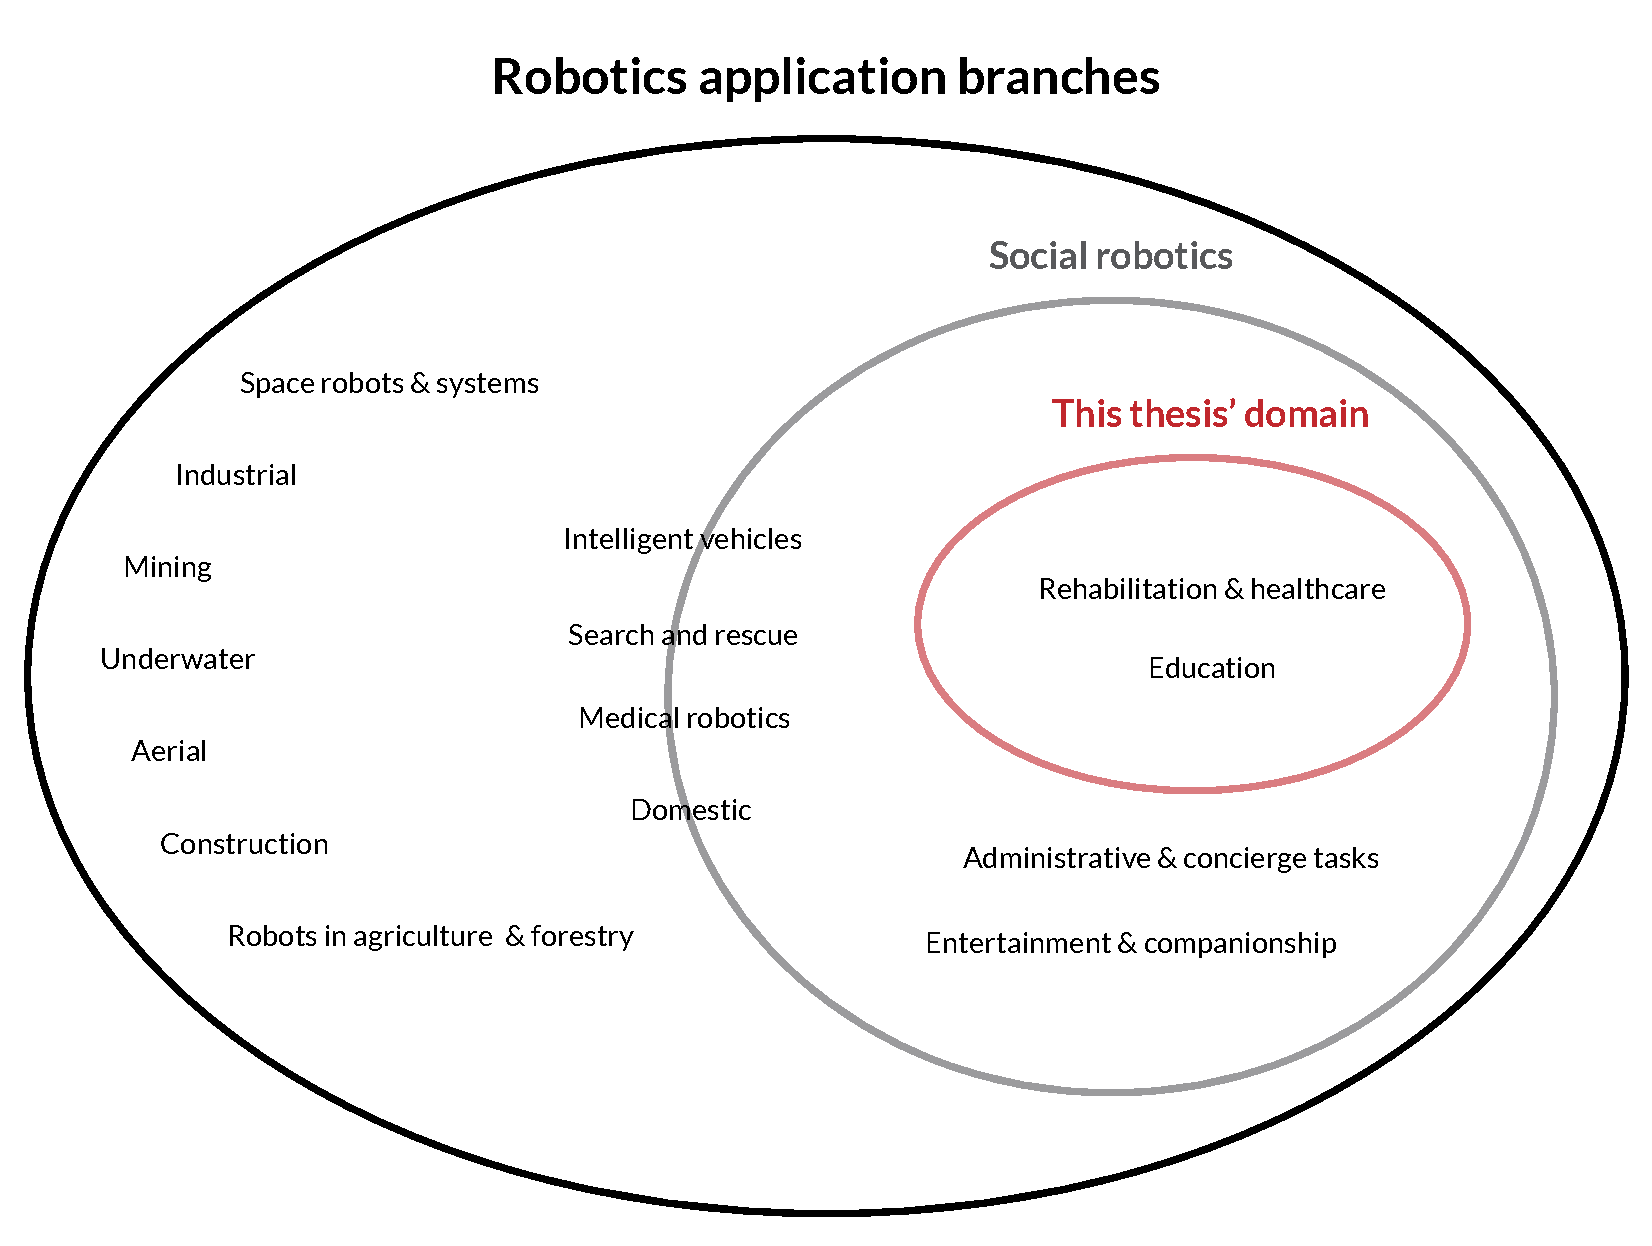
\includegraphics[scale=0.45]{images/robotics_application_branches.pdf}
  \caption{The field of robotics, adapted from \cite{Breazeal2008}. This project focuses on the rehabilitation, healthcare and education domains of robotics. Intelligent vehicles, search and rescue robotics, medical robotics and domestic robotics can be considered to be on the border of being social, which is why they are depicted partially inside the sphere of social robotics.}
  \label{fig:fieldRobotics}
\end{figure}

Autism spectrum disorder (ASD) is a disorder characterized by impaired language and communication, impaired social behavior, and narrow flexibility in daily activities \cite{frith2003autism, tetzchner, WHOautism}. Assistive sign language is a form of communication used by people with autism with limited verbal abilities \cite{puheSuomi}. Autists usually learn assistive signs early on, which is why this research examines autistic children specifically. 

Robots have been previously explored in communication therapy use with children with autism. The rationale behind using a robot for this type of therapy is that the robot's social behavior can be consistently controlled, which may make it less overwhelming for autistic people \cite{kozima2009keepon}. Additionally, children with ASDs have been observed to show more attention toward objects than to humans \cite{autismi}, and to be more interested in treatment when it involves robotic components \cite{robins2006appearance}. Research has been conducted to explore robots as tools in communication therapy for autistic children \cite{ARIA, charlie2011, boccanfuso2017low, duquette2008exploring, giullian2010detailed, goodrich2012incorporating, kim2013social, kim2015potential, kozima2009keepon,pop2013social, robins2004effects, robins2006appearance, wainer2014pilot}, and separately to teach sign language to neurotypical children \cite{taleofarobot, uluer2015new}. Combining these two elements served as the motivation to conduct this research. 

In order to examine whether a robot teaching assistive sign language to children with autism is feasible, experiments are performed with autistic children. The robot used as a platform for this solution is the open source robot InMoov, which is modified to be appropriate for this use. The InMoov is a human-sized humanoid robot torso, constructed out of 3D printed body components and gears. Its entire schematic is available under the Creative Commons license (CC-BY-NC). The original InMoov schematic was designed by Gael Langevin, and further contributions to its schematics and attached software are made by the open source community of InMoov enthusiasts \cite{inmoov}. The InMoov was selected due to availability, and to my knowledge has not been used in other academic studies.

The experiments are done in collaboration with the Satakunta hospital district in Finland. Two professionals working at the Satakunta hospital district acted as advisors for the design process presented in this thesis. These experts consulted are a speech therapist, Akuliina Lehtonen, and a neuropsychologist, Terhi Nyman. 

%%%%%%%%%%
%%%%%%%%%%


\section{Research problem}

This thesis aims to design and implement the first instance of a robot teaching assistive sign language to children with autism. This thesis explores the research problem:

\vspace{3mm}
\noindent\textbf{How should the InMoov be designed to be a tutor of assistive sign language for children with autism?}
\vspace{3mm}

This is done by first developing an understanding of autism, assistive signing, and robots in use by children with autism. With the developed knowledge, a design is constructed and tested with autistic children. This design is then evaluated. Thus, the research problem is divided into three research questions:


\vspace{3mm}

\noindent\textbf{RQ1: What are the design choices that may impact the InMoov's usefulness as a sign language tutor?}
\vspace{3mm}

\noindent\textbf{RQ2: Is the designed robot successful as an assistive sign tutor?}
\vspace{3mm}

\noindent\textbf{RQ3: How should the initial design or consequent designs be modified?}
\vspace{3mm}


The knowledge necessary to answer RQ1 is gathered in chapter \ref{chapter:background}, after which a design is constructed in chapter \ref{chapter:design}. The methods to answer RQ2 are detailed in chapter \ref{chapter:methods}, and results are examined in chapter \ref{chapter:results}. RQ3 is discussed in chapter \ref{chapter:discussion}.


%%%%%%%%%%
%%%%%%%%%%

\section{Objectives and scope of the thesis}

The objective of this thesis is to provide knowledge on the design of social robots, specifically for use in teaching assistive sign language to children with autism. 

On an empirical level, this objective is fulfilled by detailing the first pilot study of a robot teaching assistive signs to children with autism. The study examines whether the robot is successful as a tutor. Specifically, three different design conditions are compared, in order to provide knowledge on which of these three design decisions are beneficial. Additionally, future recommendations for the robot presented in this thesis, and other similar robots that could be implemented in the future, are presented based on the results from the experiments. These recommendations can help people designing robots make decisions in the future.

On a theoretical level, the objective is fulfilled by proposing a design framework for the design of social robots. Existing social robots have not been systematically and consistently designed from end-to-end, which motivated the creation of the framework. The framework is utilized as a tool during the design process presented in this thesis, and it can be utilized in the design of any social robot in the future. To my knowledge, this is the only design framework that details the entire design process of a social robot. In this thesis, the framework is used specifically to modify the design of the robot InMoov to be suitable for teaching assistive signs to children with autism. The description of this process serves as an example of how the framework can be utilized.

Due to the large base of theoretical knowledge that is presented in this thesis, the experiments themselves are kept small in size. Additionally, organizing experiments with autistic children is challenging, which is why only 10 participants' data are analyzed. To provide definitive results on the usefulness of a robot in this type of use, clinical level studies would need to be conducted. However, due to the pilot nature of the study, a small number of participants is deemed as useful to provide the first steps into a previously unknown niche branch of robotics.

Due to the narrow scope of the experiment itself, the design framework is considered as the most important contribution of this thesis.


%%%%%%%%%%
%%%%%%%%%%

\section{Structure of the thesis}

The second chapter is a literature review presenting academic literature on autism and the communication impairment associated with it, social robots previously in used in communication therapy, and social robots previously used as teachers of sign language. The chapter ends with the theoretical knowledge being synthesized into design guidelines for the robot.

Following the discussion of the background, the design for the robot is presented. A design framework is introduced as a tool to make design decisions about different dimensions of a social robot. In this thesis, the robot InMoov is situated into the design framework, and modifications are made to it according to the design guidelines established in chapter \ref{chapter:background}.

Chapter \ref{chapter:methods} presents the methods to be used to study the modified InMoov teaching assistive signs to children with autism. The research setting, process and methodology are presented.

Results of the experiments are presented in chapter \ref{chapter:results}. Both quantitative and qualitative results are analyzed.

Following the results of the study, the chapter \ref{chapter:discussion} discusses the answers to the research questions. Limitations of the study are detailed thoroughly. Practical and theoretical implications, as well as suggestions for future research are discussed. Finally, a conclusion is provided.


\chapter{Background}
\label{chapter:background} 


This chapter examines how autism manifests in children, how it affects their communication skills, and what assistive sign language is. This chapter also examines what research has already been done with social robots as communication therapy tools for autistic children, and social robots as teachers of sign language. At the end of this chapter, this knowledge is synthesized into five design guidelines, which will guide the design process of the robot in chapter \ref{chapter:design}.


%%%%%%%%%%
%%%%%%%%%%


\section{Autism in children}


Autism or autism spectrum disorder (ASD) is a developmental disorder which is characterized by impaired social behavior, impaired communication and language, and a narrow range of interests and activities that are unique to the individual and carried out repetitively \cite{WHOautism}.  The intervention described in this thesis is targeted at improving impaired communication.

In 2017, the World Health Organization reported that worldwide, 1 in 160 children has an autism spectrum disorder \cite{WHOautism}. According to a Danish study, ASD diagnoses have been increasing, with incidence rates rising from 9.0 to 38.6 per 100 000 people from 1995 to 2010 in Denmark. Increases were most pronounced among adolescents, adults and females \cite{jensen2014time}. Diagnoses of ASD are also increasing globally. This apparent increase could be due to improved awareness, expansion of diagnostic criteria, or better diagnostic tools and improved reporting \cite{WHOautism}.

ASD begins in childhood, and in most cases the condition is apparent during the first five years of a child's life. Autism usually persists into adolescence and adulthood. The level of functioning among individuals with ASD is highly variable, and ability ranges from profound cognitive impairment to superior performance in certain areas \cite{WHOautism}. Research has shown that the level of functioning of adults with ASDs depends on how well they were using language before school age \cite{tetzchner}.

Early interventions targeted at improving the speech, communication or behavior of the autist are aimed at improving quality of life, rather than curing the disorder. When provided early enough, interventions can improve the person's self-care, communication and social skills \cite{tetzchner}. Due to this, the intervention introduced in this thesis focuses on children.

%%%%%%%%%%
%%%%%%%%%%

\subsection[Communication and language difficulty as a characteristic of autism spectrum disorder]{Communication and language difficulty as a \\characteristic of autism spectrum disorder}

50 \% of children with autism remain functionally mute in adulthood \cite{puheSuomi, peeters1999autism}. For those that do learn to speak, the development of language is often delayed, and the level of language is highly variable \cite{puheSuomi}.

According to the current understanding, the key problem of autism is a lack of ``Theory of Mind'', which means that people with autism have trouble recognizing that other humans have thoughts and feelings, and have trouble anticipating others' behavior \cite{baron1985does, frith2003autism}. People with autism also experience problems in integrating pieces of information into a coherent whole. These core problems contribute to the problems of communication, social interaction and flexibility that people with ASDs experience \cite{frith2003autism}. Problems experienced in social interactions discourage autistic people even further from making an effort, which in turn minimizes opportunities to learn communication and social skills, creating a negative feedback loop \cite{autismi}.

To avoid this loop, teaching autistic children communication and social skills needs to be clear and structured so as not to confuse and distress the person even further. Therapy for children with ASDs often focuses on teaching basic social skills such as eye contact, turn taking, joint attention and emotion recognition \cite{autismi}. Because problems in speech can be anticipated, therapy for people with autism often includes practicing using other forms of communication, such as using assistive sign language, gestures, picture symbols or photos \cite{puheSuomi, tincani2004comparing}. These forms of communication can be used either as alternative communication, which replaces speech, or augmentative communication, which supports speech \cite{puheSuomi}. In the intervention presented in this thesis, the focus is specifically on assistive sign language, which is a form of augmentative communication.


%%%%%%%%%%
%%%%%%%%%%

\subsection{Assistive sign language as a communication method for people with autism spectrum disorder}

Signing is the most used form of both alternative and augmentative communication used in Finland \cite{puheSuomi} and globally \cite{tetzchner}. Signing can hasten the acquisition of speech for some autistic individuals, since during signing, visual and motoric memory support the auditory memory used for speech \cite{bonvillian1981sign, autismi}. Early sign language teaching has been shown to advance the development of children, especially their language, cognitive and social skills \cite{puheSuomi}. 

Assistive sign language, which is a form of augmentative communication, is used simultaneously with speech, in support of it. Individual signs are borrowed from Finnish sign language, but the grammar and structural rules associated with Finnish sign language are not used. The most important words of sentences are signed simultaneously as the words are spoken \cite{puheSuomi}. According to speech therapist Lehtonen, who works with autistic children, the most important word is determined by the context. For example, when saying ``Let's go to the kitchen to eat.'', the most important word can be ``kitchen'' if eating is usually done somewhere else, or it could be ``eat'' if eating is being done at an exceptional time, and the kitchen is usually reserved for other activities  (A. Lehtonen, personal communication, June 25, 2018).

Finnish sign language signs are constructed of four components: hand shape, placement, movement and orientation. In addition to hands, facial expressions and body posture are also used to communicate signs. Mouth shape can also be used to communicate \cite{puheSuomi}. According to speech therapist Lehtonen, the hands are most important in assistive signing. Facial expressions can be used to communicate the tone of the statement. For example, saying ``My house burned down.'' requires a frown, but ``We have a nice new house.'' requires a smile, even if the word ``house'' is what is being signed in both cases (A. Lehtonen, personal communication, June 25, 2018).  

Assistive signing has advantages over other augmentative communication systems, such as graphical picture systems. Signing needs no external tools. Especially for a small child, carrying around equipment such as an image communication system would not be practical \cite{puheSuomi}. However, symbolic pictures or photos do not share the disadvantage of being hard to understand for people who have no experience with them \cite{tetzchner}.

Autistic individuals can have difficulties learning to sign. Motoric difficulties sometimes exhibited by autistic individuals may play into difficulties signing \cite{autismi}. Many autistic children have spacial dyspraxia, a coordination disorder, which makes it difficult to perceive and produce signs. For example, signs may be performed slowly \cite{bonvillian1981sign}, the fingers of the individual may be stiff, or the trajectory of movements may be hard to control. In addition to this, some autists may have trouble recalling signs from memory quickly enough to be used in spontaneous conversation \cite{puheSuomi}.

These factors can lead to assistive signs being individualistic, and only recognizable by the individual's family and others closely in contact with them \cite{autismi}. When the autistic individual meets a new person, this person should be taught the unique signs that the autist is using \cite{puheSuomi}.

%%%%%%%%%%
%%%%%%%%%%


\subsection[Current methods and challenges of learning assistive signs as a child with autism spectrum disorder]{Current methods and challenges of learning \\assistive signs as a child with autism spectrum disorder}

Learning a new method of communication requires co-operation of the child's speech therapist, loved ones and other educators the autistic child may have \cite{tetzchner}. Learning assistive signs is difficult from a book or from videos, since signs require spacial moves. This means that the individual usually needs a physical teacher to learn signs. To achieve best results, the people close to the autistic person should learn and use assistive sign language in everyday situations \cite{bonvillian1981sign,puheSuomi}. Sign language tutoring should be started as early as possible, in order to achieve the best level of signing and speech possible \cite{bonvillian1981sign}.

Almost all autistic people are capable of learning at least a few signs, and usually in a short time \cite{bonvillian1981sign, tetzchner}. Those individuals who benefit the most from signing can spontaneously produce long signed sentences after years of speech therapy. For some exceptional individuals, remembered signs can exceed hundreds. It has been shown that even the lowest functioning autists can acquire from five to ten signs with a year of studying. Even this level of signing can greatly improve quality of life \cite{tetzchner}.

Goals for learning sign language should be defined according to the individual, to avoid unrealistic goals that would deter both student and teacher from further study. Therapy sessions should be designed and signs to be learned should be chosen according to the needs of the individual, as autism can present very differently across individuals. The individual's needs and interests need to be taken into account \cite{bonvillian1981sign, tetzchner}.

Taking breaks from learning can have adverse effects, as the child may forget already learned signs if they do not have enough repetitions and practice. Moving or change of environment can also create problems for learning. If the teacher changes, the new teacher may not have sufficient knowledge of what the child has learned, and what they do not yet know. If a teacher is unfamiliar with a child, they may be unable to recognize unique signs that a child is using. Such inconsistencies in teaching will frustrate the child, which in autism can often lead to behavioral problems and anger, which will further degrade the quality of learning \cite{tetzchner}. These are problems that could be addressed with new teaching methods.

Generalization is another challenge in learning signs. Generalization is the process of transferring learned signs into use in everyday life. To aid generalization, spontaneity of communication should be emphasized, to encourage the child to take initiative and be an independent communicator, rather than attempting to communicate only when prompted \cite{carr1983acquisition}. This can be done by combining the learning of speech and communication with everyday situations, and practicing with the people present in the child's everyday life. This requires co-operation with the individual's loved ones and other educators \cite{carr1983acquisition, tetzchner}.


%%%%%%%%%%
%%%%%%%%%%

\section{Social robots as tools for autistic children and sign language tutors}

Social robots have been used as communication therapy tools with autistic children. They have also been explored as tools to teach sign language to children. This thesis presents the first known instance of using a social robot to teach assistive sign language to autistic children, as a form of communication therapy. 


%%%%%%%%%%
%%%%%%%%%%

\subsection[Robots as communication therapy tools for autistic children]{Robots as communication therapy tools for \\autistic children}

A significant amount of research has been done in the field of robotics with autistic children as a user group. The ability to consistently control a robot's social behavior make them potentially interesting tools for communication practice for autistic children \cite{kozima2009keepon}. Additionally, autistic children have been observed to show more attention toward objects than to humans when playing \cite{autismi}, and to be more interested in treatment if it involves technological or robotic components \cite{robins2006appearance}. These observations have led researchers to explore robots as tools in therapy.

A variety of robots have been used in communication therapy with autistic children, nine of them are presented in table \ref{table:robots}. These robots have either been specifically built for research with autistic children, built for research and adapted for autistic children, or built for commercial purposes but adapted for use in research with autistic children. Additionally, robots that have been built to be commercially sold for use in communication behavior therapy with autistic children exist. However, no research on those robots is available, so they are not included here. 

The list of robots in table \ref{table:robots} is not exhaustive, as other robots used in autism communication therapy also exist. The robots presented here were chosen on the basis of relevant literature being made available. The robots examined here were used in experiments with autistic children specifically with the purpose of improving their communication skills. The purpose of examining these robots is to gain theoretical knowledge about robots in this use, in order to make design decisions about the robot to be used in this experiment, and the experimental set-up to be used.


\clearpage
\newcolumntype{L}[1]{>{\raggedright\let\newline\\\arraybackslash\hspace{0pt}}m{#1}}

\urlstyle{same}

  \begin{longtable}
      {L{1.5 cm}  L{2.25cm}  L{3cm}  L{2.25cm}  L{2.75cm}} \hline Robot &  Category & Studies and educational objectives & Image & References \\
      \hline
      \centering
      
      %built for autism research
      
      %Tito
      Tito & built for research with autistic children & interaction games \cite{duquette2008exploring}  & \parbox[c]{1em}{\vspace{0.1cm}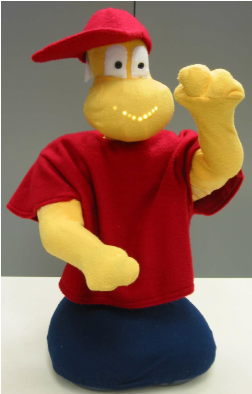
\includegraphics[width=1in]{images/Tito.png}
      \vspace{0.1cm}} & 
      \scriptsize{Creators: Audrey Duquette, François Michaud and Henri Mercier. Image: Assistive Technologies and Child-Robot Interaction – Scientific Figure on ResearchGate. Available from: \url{https://www.researchgate.net/Tito_fig2_249766819}}\\
      
     
      
      %Troy
      Troy & built for research with autistic children & pilot study \cite{giullian2010detailed}, long-term therapy \cite{goodrich2012incorporating}  & \parbox[c]{1em}{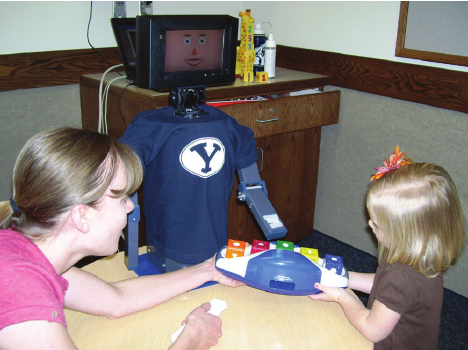
\includegraphics[width=1in]{images/Troy-BYUs-humanoid-robot.png}
      \vspace{0.1cm}} & 
      \scriptsize{Creators: J. Alan Atherton and Michael J. Goodrich. Image: Visual robot choreography for clinicians – Scientific Figure on ResearchGate. Available from: \url{https://www.researchgate.net/Troy-BYUs- humanoid-robot_fig1_224243058}}\\

      %Charlie
      Charlie  & built for research with autistic children & pilot study \cite{charlie2011}, interaction games \cite{boccanfuso2017low} & 
      \parbox[c]{1em}{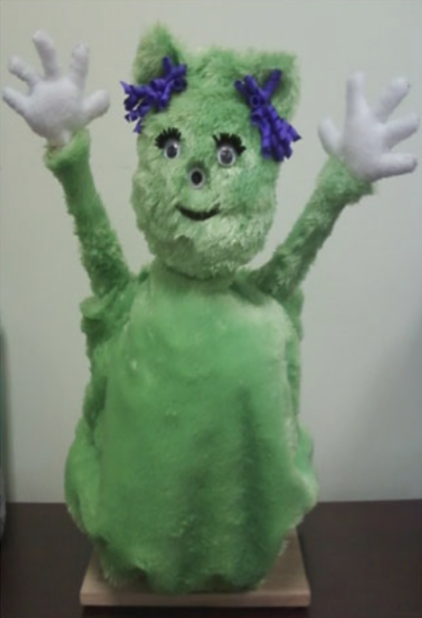
\includegraphics[width=1in]{images/charlie.png}\vspace{0.1cm}} & \scriptsize{Creators: Laura Boccanfuso and Jason M. O'Kane. Image: With kind permission from Springer Science + Business Media: Intl J Soc Rob, \cite{charlie2011}.} \\
      
      
      %built for research
      
      
      %Robota
      Robota  & built for research & long-term therapy \cite{robins2004effects}, effect of appearance of robot \cite{robins2006appearance} & \parbox[c]{1em}{      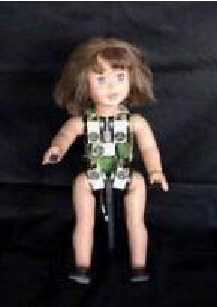
\includegraphics[width=1in]{images/Robota-Billard-et-al-2006.png}
      \vspace{0.1cm}} & 
      \scriptsize{Creators: Aude Billard at Adaptive Systems Laboratory at University of Lausanne. \cite{robotaRef}. Image: KASPAR – A Minimally Expressive Humanoid Robot for Human–Robot Interaction Research – Scientific Figure on ResearchGate. Available from: \url{https://www.researchgate.net/figure/Robota-Billard-et-al-2006_fig4_255601703}} \\
      
      
      %Keepon
      Keepon  & built for research & freeform interaction \cite{kozima2009keepon}  & \parbox[c]{1em}{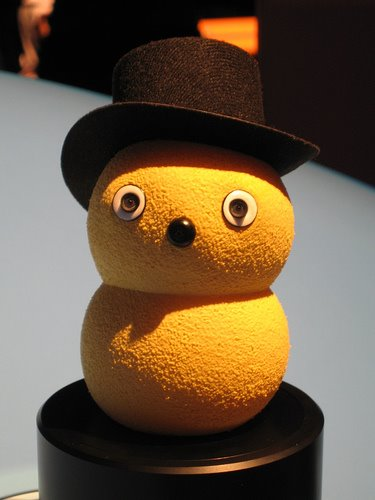
\includegraphics[width=1in]{images/KeeponTophatNextfest2007.jpg}
      \vspace{0.1cm}} & 
      \scriptsize{Creators: Hideki Kozima while at the National Institute of Information and Communications Technology. Image: Ilikedudes, from Wikimedia Commons.}\\
      
      
      %Probo
      Probo  & built for research & independent communicating during social stories \cite{pop2013social} & \parbox[c]{1em}{      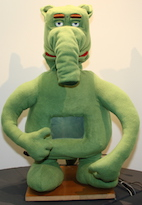
\includegraphics[width=1in]{images/probo.jpeg}\vspace{0.1cm}} & \scriptsize{Creators: Vrije Universiteit Brussel. Image: Probo, Vrije Universiteit Brussel \cite{ProboRef}.} \\
      
      
      %Kaspar
      Kaspar  & built for research  & interactive games \cite{wainer2014pilot}, co-creating autism interventions \cite{huijnen2017implement} & \parbox[c]{1em}{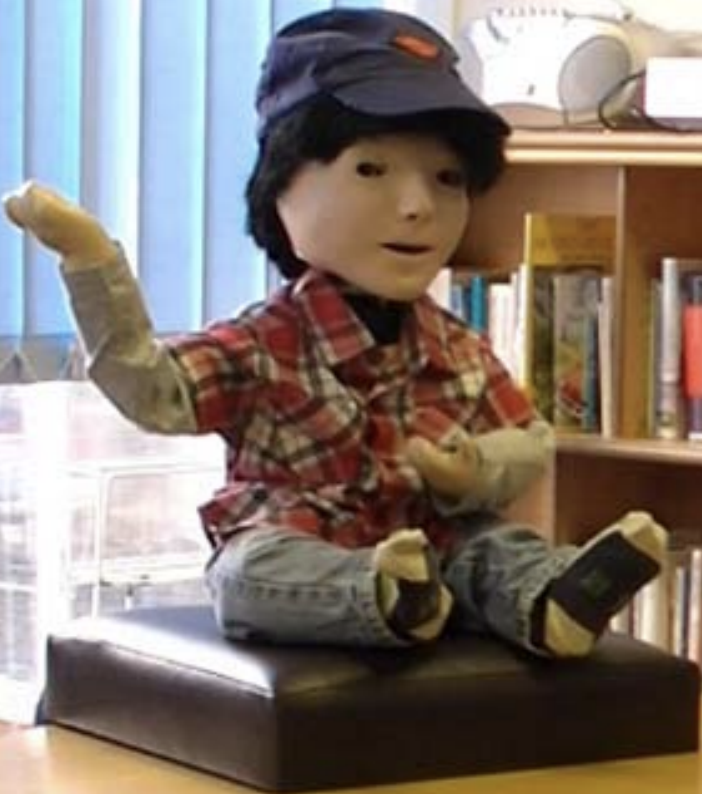
\includegraphics[width=1in]{images/kaspar.png}
      \vspace{0.1cm}} & 
      \scriptsize{Creators: Adaptive Systems Research Group at University of Hertfordshire \cite{kasparRef}. Image: Luke Wood, Kerstin Dautenhahn, A. Rainer, Ben Robins, Hagen Lehmann and Dag Sverre Syrdal. Used under a Creative Commons Attribution licence.}\\
      
      
      
      
      %built for commercial purposes
      
      %Nao
      Nao  & commercial, adapted for research & attention direction \cite{ARIA} & \parbox[c]{1em}{      \vspace{0.1cm}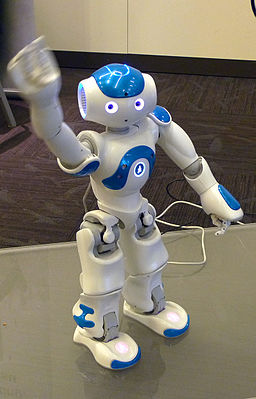
\includegraphics[width=1in]{images/NAO_waving.JPG}\vspace{0.1cm}} & \scriptsize{Creators: Aldebaran Robotics, acquired by Softbank Robotics \cite{NaoRef}. Image: Anonimski [CC0], from Wikimedia Commons.} \\
      
      
      %Pleo
      Pleo  & \vspace{0.1cm}commercial, adapted for research &robot as an embedded reinforcer of social behavior during semi-structured interactions \cite{kim2013social}, effect of positive affect during semi-structured interactions \cite{kim2015potential}\vspace{0.1cm}  & \parbox[c]{1em}{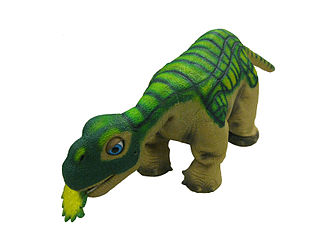
\includegraphics[width=1in]{images/Pleo_robot.jpg}\vspace{0.1cm}} & \scriptsize{Creators: Innvo Labs \cite{PleoRef}. Image: Jiuguang Wang, from Wikimedia Commons.}\\
      

      \hline
      
      
      \caption{Nine robots used in interventions targeting improvement of communication skills for children with ASDs. Pilot studies examining the robot's usability for this purpose, and studies where the robot was interacting with children with ASD are included. Robots are organized by category: robots that were designed specifically for use by children with autism first, robots that were designed for research and adapted for use by children with autism next, and robots that were designed for commercial use but adapted for research for children with autism last. Inside these categories, robots are organized according to oldest relevant research.}
      \label{table:robots}
    
  \end{longtable}


These nine robots are discussed in more detail below.


%autism robots
%Tito
\subsubsection{Tito}

Tito is a low-cost, custom-made robot for autism therapy created at the University of Sherbrooke. Tito is a small, cartoon-like robot that wears human clothes. 

Tito was used in an experiment to facilitate reciprocal interaction, such as imitative play. The experiment involved four low-functioning autistic children, two of whom interacted with the robot and two with a human mediator. The mediators executed imitation play patterns on three levels: facial expressions, body movements, and familiar actions with or without objects. Experiments were conducted with pre-programmed behaviors consisting of motion and vocal messages \cite{duquette2008exploring}.

The study measured shared focused attention and shared conventions, as well as absence of sharing, to determine the success of the interaction. The study showed that the robot mediator induced increased shared focused attention, visual contact and physical proximity, and children paired with it smiled more. However, children paired with the human mediator showed more shared conventions, such as imitation of body movements and familiar actions \cite{duquette2008exploring}.


%Troy
\subsubsection{Troy}

Troy was built at Brigham Young University for use in autism therapy. It is simple and mechanical in appearance, wears a human's shirt and pants, and has a screen as a face, on which different emotions can be displayed. Troy's behaviors were designed to encourage turn-taking and imitation in the child interacting with it \cite{goodrich2011case}.

The baseline of Troy in use for autism therapy was determined in a small study in 2010. The study showed that the robot could be controlled effectively during a therapy session, and that children seemed to treat it as a ``social other'' \cite{giullian2010detailed}.

In 2012, Troy was incorporated into an autism therapy team in longitudinal studies with two children with autism. The experimental set-up had a ``low-dose'' approach, where the robot was used for only 10 minutes during a 50 minute therapy session. The study noted increase in socially engaged behaviors as compared to before the study. The children also showed more interaction with the clinician after the treatment. Increase in greeting, symbolic play and sharing toys was also noted, as well as a decrease in restricted interests and repetitive behaviors \cite{goodrich2012incorporating}.


%Charlie
\subsubsection{Charlie}

Charlie is a low-cost robot, designed for use by children with autism in communication therapy, built at the University of South Carolina. The robot was explored in a pilot study in use with typically developing children in 2011. The robot taught imitation skills via the games ``Imitate Me, Imitate You'', and ``Pass the Pose''. Children interacted either only with the robot, imitating its movements and vice versa, or interacting with another child through the robot. The pilot succeeded as a proof-of-concept, as the neurotypical children interacted with the robot willingly, and it succeeded in operating as planned, detecting the children's faces and hands successfully \cite{charlie2011}.

At Yale university, Charlie was incorporated into an ASD-intervention within clinical methodology. The research noted improvements in communication and social interaction in the children, which were measured prior and after the interventions. The interventions focused on child-led interaction games \cite{boccanfuso2017low}.


%research robots
%Robota
\subsubsection{Robota}

Robota is a small, female-looking, doll-like robot, that was built at Adaptive Systems Laboratory at University of Lausanne \cite{billard2003robota}. Robota was designed to emphasize its humanoid aspect, and to have an especially human-like appearance for its face \cite{billard2006building}. 

Robota was not originally designed for use by children with autism, but has been applied as assistive technology in behavioral studies with low-functioning autistic children \cite{billard2006building}. Robota has been used in studies with autistic children by the AuRoRA research group, ``Autonomous Robot as a Remedial tool for Autistic children'', at the University of Hertfordshire \cite{robins2004effects, robins2006appearance}. AuRoRA is a research project initiated in 1988 at the University of Hertfordshire, studying the use of robots as tools that may serve an educational or therapeutic role for children with autism. Robota is autonomous, and has been taught sequences of actions and vocabulary using machine learning algorithms. Robota can react to touch by detecting passive motion of its limbs and head through its potentiometers \cite{robins2004effects}. 

AuRoRa used Robota to examine the long-term effects of use of a social robot in therapy with autistic children. This experiment was designed in response to the observation that one-time experiments are not likely to accurately predict what effects long-term therapy with robots could have. The change over time of eye gaze, touch and imitation in social interactions were observed. The experiment showed that all four children involved opened up socially to the robot and willingly interacted with it. The experiments also showed that conditions prior to arriving at the therapy, for example an unplanned change in schedule, which can be stressful for an autistic child, can significantly affect the child's behavior during the session \cite{robins2004effects}.

Robota was also used by AuRoRA to explore whether a robot's appearance matters in the interaction between an autistic child and the robot. The study showed that children with ASD have a preference for plain, featureless robots over robots with human-like features. The study compared Robota with a robotic appearance with a dressed-up, human-like Robota. Children displayed more social and pro-active behavior toward the plain Robota \cite{robins2006appearance}. Robota's appearance was subsequently changed to be more simple and robotic \cite{billard2006building}.


%Keepon
\subsubsection{Keepon}

Keepon is a small robot, designed for non-verbal, simple communication with children in order to study, test and elaborate on psychological models of development of social intelligence. It was designed by Hideki Kozima's research team at the National Institute of Information and Communications Technology in Kyoto. The minimalistic design has a yellow ``snowman''-like form, and was created after the same researchers determined that their toddler-sized and mechanical robot Infanoid provided too much stimulus for autistic children, and overwhelmed them so that they could not interact with it. Keepon has both an autonomous and teleoperated operation mode \cite{kozima2009keepon}.

Keepon has been used with both normally developing and autistic children. With autistic children, Keepon was observed to become regarded as a social actor by the children, increasingly toward the end of the their 15 interaction sessions over five months. The authors suggest that this indicates that autistic children do in fact have a motivation for sharing and exchanging mental states with others, contrary to popular belief (cf. \cite{carpenter2005role}). The researchers argue that when a robot is carefully designed to express its mental states in a way that is comprehensible to autistic children, they will establish a social relationship with it. Kozima argues that simple robots can facilitate exchange of mental states in children with autism, implying that the major social difficulties experienced by autistic children stem from difficulty of sifting out socially meaningful information in human interactions, rather than from lack of motivation \cite{kozima2009keepon}.


%Probo
\subsubsection{Probo}

The ``huggable robot'' Probo was designed at Vrije Universiteit Brussel, to be used by children in hospital contexts as a tele-interface for entertainment, communication and medical assistance. The social robot is a soft, elephant-like creature, with a screen in its stomach \cite{saldien2008design}. It has been adapted for research with autistic children.

An experiment conducted with 20 autistic children revealed that the children needed fewer communication prompts from the robot than a computer display, in order to respond to prompts given during a social story. The prompts were hierarchical, ranging from verbal to gestural and physical. The study examined the degree of independence of expressing social abilities such as asking questions, eye gaze, asking for help, and greeting. The use of Probo increased the independence of children expressing their social abilities \cite{pop2013social}.


%Kaspar
\subsubsection{Kaspar}

Kaspar, “Kinesics and Synchronization in Personal Assistant Robotics”, is a child-sized minimally expressive humanoid robot that has been developed by the Adaptive Systems Research Group at University of Hertfordshire. Kaspar is male-looking, has elastic skin and wears children's clothes. Kaspar was specifically designed to study human-robot interaction, with the aim of being able to signal emotions in a minimally expressive way \cite{dautenhahn2009kaspar}.

The AuRoRA research group has used Kaspar in several studies \cite{auroraProject}. Kaspar has been used to provide a predictable and repetitive experience of communication, which aims to be more comfortable for autistic children. Kaspar can be used to teach autistic children communication skills such as engaging in direct eye contact or taking turns. Kaspar also provides an enjoyable play context for the child to build their social skills \cite{kasparImpact}.

In the latest study by AuRoRA, Kaspar was used to explore the differences of a robot and a human playing partner in an interactive game with autistic children. The study concluded that children were more entertained by the robot, but more collaborative with human partners \cite{wainer2014pilot}.

Kaspar has also been used at other universities, such as Zuyd University of Applied Sciences, where it was used to co-create autism interventions together with autistic children, their parents and professionals of the field \cite{huijnen2017implement}. 


%commercial robots
%Nao
\subsubsection{Nao}

Nao is a commercial robot developed by Aldebaran Robotics in 2006, later acquired by Softbank Robotics \cite{NaoRef}. Nao is a small humanoid robot. It has been adapted as a research platform, due to its programmability.

In 2013, Nao was used as a tool to test robot-mediated joint attention skills with autistic children. The research involved creating a hierarchical structure of prompts executed by the robot to direct the child's attention. The study determined that children with autism showed a stronger preference toward robots over humans when compared to neurotypical children. Children with ASD also needed more prompts from the robot to successfully direct their attention than neurotypical children \cite{ARIA}.

The study concluded that using robots to teach social skills was promising, and they could be used to take advantage of autistic children's non-social attention preference. The study raised questions of how to generalize skills learned with the robot into everyday life \cite{ARIA}.


%Pleo
\subsubsection{Pleo}

Pleo is a small animatronic dinosaur toy, developed by Innvo Labs \cite{PleoRef}. Pleo has rudimentary sight, touch, temperature and motion sensors, and can understand basic voice commands.

The robot Pleo has been used to study the behavior of autistic children in semi-structured interactions \cite{kim2013social, kim2015potential}. Children were found to show more utterances toward an accompanying adult, when interacting with the robot in comparison to a computer screen \cite{kim2013social}. Researchers also noted more positive affect displayed by the child when interacting with the robot than with a human partner. Positive affect was defined as enjoyment or happy excitement. The study also noted that positive affect was related to greater autism severity, which meant that robots have the potential to be effective in interventions with lower functioning autistic individuals \cite{kim2015potential}.


%%%%%%%%%%
%%%%%%%%%%

\subsection{Sign language tutoring with social robots}

To my knowledge there is only one research group, the Cognitive Social Robotics Laboratory at Istanbul Technical University in Turkey, that has been studying robots as teachers of sign language to children \cite{CSRLpublications}. These studies have not researched the use of robots to teach sign language to children with ASD.



\subsubsection{Nao}

A study by the research group in 2011 explored the use of the Nao as a teacher of sign language for neurotypical children with normal hearing. In this study, non-verbal communication and imitation based interaction games between the robot and child were used to evaluate the children's ability to learn sign language from Nao \cite{taleofarobot}. Children readily imitated the robot during the study. The study referenced a previous study by the same research group, where the physical presence of a robot (Kaspar in particular) was determined to be more effective than a video of a robot \cite{kose2009effects}, and noted that this new study confirmed the result. The use of video as a sign language teaching method for children was not as effective as the use of a robot, because it lacks the social interaction dimension. The researchers also found that the effects of the physical limitations of the robots were diminished when the children had a relevant context or story for the signs \cite{taleofarobot}. 

This study did not research the use of the robot with children with ASD. The main observation from the study in the context of this thesis is that successful imitation of the robot by the human user can be used as a measure of successfully learning sign language from the robot.


\subsubsection{Robovie R3}

\begin{figure}
\centering
\urlstyle{same}
  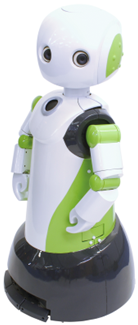
\includegraphics[width=1in]{images/robovieR3.png}
  \caption{Robovie R3. Creators: VStone \cite{Vstone}. Image: Advanced Telecommunications Research Institute International. Available at: \url{http://www.atr.jp/topics/press_100420_j.html}}
  \label{fig:robovie}
\end{figure}

A study done by the same research group in 2015 detailed how a five-fingered robotic platform, Robovie R3, was used to teach Turkish sign language to children. Robovie R3 is a humanoid robot with sophisticated hands, developed by Japanese company Vstone \cite{Vstone}. Robovie R3 is presented in figure \ref{fig:robovie}.

The study used imitation-based interaction games to tutor both children with hearing loss and children with normal hearing. The study aimed to establish interaction between the child and the humanoid robot through imitation and turn-taking. Robovie R3 was determined to be both successful in accurately demonstrating signs, and teaching the children \cite{uluer2015new}.

The study's robot was able to produce a set of 10 signs, chosen from a sub-set of daily used words. The same signs were used in the previous study with the robot Nao, and thus took into account Nao's physical limitations \cite{taleofarobot}. Due to its greater physical flexibility, Robovie R3 was determined to be a better sign language teacher than Nao \cite{uluer2015new}.

The robot was not examined in use by autistic children. The most important learning from this study in the context of this thesis is that imitation and turn-taking games were determined to be useful methodologies in a study examining whether users can learn sign language from a social robot.


\subsection{Design guidelines}

The robots discussed here, along with the observations and recommendations made in the studies, are used as a base to formulate design guidelines for a robot to be used to teach assistive signing to children with autism. In addition to this, explicit design recommendations and guidelines made by researchers for the design of social robots \cite{bartneck2004design}, and for robots specifically for use by autistic children \cite{designSpaces, giullian2010detailed, michaud2003characteristics, robins2007eliciting} are taken into account. Knowledge and research presented earlier in this chapter on how autism manifests and is treated in children is also applied to formulate the design guidelines.

The design guidelines will be used to guide the design process of the robot presented in this thesis, and will be utilized in the process of making explicit design decisions in the next chapter. While these guidelines have been developed with this particular application in mind, where the robot is used to teach assistive sign language to children with autism, these guidelines can be utilized in the design of robots for use by children with autism in general.

The design guidelines are:


\begin{itemize}

  \item \textbf{Simple form} \cite{charlie2011, boccanfuso2017low, designSpaces, duquette2008exploring, frith2003autism, giullian2010detailed, robins2007eliciting, robins2006appearance, kozima2009keepon}
  
  \item \textbf{Consistent, structured, simple behavior} \cite{bartneck2004design, charlie2011, boccanfuso2017low, billard2006building, designSpaces, duquette2008exploring, frith2003autism, giullian2010detailed, kim2013social, kim2015potential, kozima2009keepon, robins2007eliciting}
  
  \item \textbf{Positive, supportive, rewarding experience and environment} \cite{ARIA, charlie2011, boccanfuso2017low, carr1983acquisition, giullian2010detailed, huijnen2017implement, kim2015potential, kozima2009keepon, michaud2003characteristics, pop2013social, robins2004effects, robins2007eliciting, wainer2014pilot}
  
  \item \textbf{Modular complexity} \cite{ARIA, billard2006building, bonvillian1981sign, designSpaces, duquette2008exploring, giullian2010detailed, pop2013social, robins2007eliciting, robins2006appearance, tetzchner}
  
  \item \textbf{Modular specific to child's preferences} \cite{designSpaces, bonvillian1981sign, giullian2010detailed, robins2007eliciting, tetzchner}
  
\end{itemize}

The design guidelines are discussed in more detail below. Details on how the robots discussed in table \ref{table:robots} fulfill the design guidelines are presented in table \ref{table:guidelines}. The first three robots – Tito, Troy and Charlie – were designed specifically for use autistic children. Design guidelines are marked as fulfilled on the basis that a study conducted with the robot explicitly mentions the design condition being implemented or having pre-existed. Some robots that are introduced do exhibit realization of the design guidelines even if they are not explicitly mentioned. However, this is entirely up to the judgment of the observer, so these robots are not marked as following the design guidelines. For robots with multiple implementations across studies, if any implementation mentions the design guideline, they are included.


\begin{table}
 \bgroup
  \def\arraystretch{2}
  \centering
  \begin{tabular}{|p{2cm}|c|c|c|c|c|c|c|c|c|}
    \hline
     & 
    \scriptsize{Tito} &
    \scriptsize{Troy} &
    \scriptsize{Charlie} &
    \scriptsize{Robota} &
    \scriptsize{Keepon} &
    \scriptsize{Probo} &
    \scriptsize{Kaspar} &
    \scriptsize{Nao} &
    \scriptsize{Pleo} 
    \\\hline
    %\hline
    \scriptsize{Simple form} & x & x & x & x & x & – & – & – & – \\
    \scriptsize{Consistent, structured, simple behavior} & x & x & x & x & x & – & – & – & x \\
    \scriptsize{Positive, supportive, rewarding experience and environment} & – & x & x & x & x & x & x & x & x \\
    \scriptsize{Modular complexity} & x & x & – & x & – & x & x & x & –  \\
    \scriptsize{Modular specific to child's preferences} & – & – & – & – & – & – & / & – & – \\
     \hline
  \end{tabular}
  \caption{This table details how the robots presented in table \ref{table:robots} follow the established design guidelines in their relevant studies. If the robot follows a design guideline, it is marked with an ``x'', if they do not, it is marked with a ``–''. The ``/'' indicates that this is an emerging realization of a design guideline.}
  \label{table:guidelines}
  \egroup
\end{table}


\subsubsection{Simple form}

As discussed previously in this chapter, people with autism have problems with forming a holistic perception, meaning they have problems integrating different stimuli into a ``wholesome'' experience, and may instead fixate on isolated features \cite{designSpaces, frith2003autism, giullian2010detailed}. To avoid overstimulation, social robots designed for use by autistic children should be kept simple and predictable in their appearance \cite{designSpaces, kozima2009keepon, robins2007eliciting}. Additionally, an appearance that is too life-like and close to a human could even unnecessarily limit the robot and restrict its functionalities \cite{designSpaces}.

Robots examined in table \ref{table:robots} which have been designed specifically for use by autistic children have all been kept simple in form and appearance, as seen in table \ref{table:guidelines}. The robot Charlie was created to have simple, toy-like and friendly appearance to more easily attract the attention of a child, and to appear approachable and not intimidating \cite{charlie2011, boccanfuso2017low}. The robot Tito was described by researchers to be simple and human-like in appearance \cite{duquette2008exploring}. The robot Troy was designed to not be overly realistic, and to have a simple and mascot-like appearance. It was designed to have a mechanical appearance in order to be discernable as a robot, but not too mechanical so that the child would not become fixated on its components. The robot's face, which is a computer screen, has a cartoonish and simple design \cite{giullian2010detailed}.

Robota, a robot applied to behavioral studies with autistic children, was especially designed to be humanoid in appearance \cite{billard2006building}. However, it was later discovered in a study with Robota that children preferred it to have a simpler, robotic appearance \cite{robins2006appearance}. The appearance was changed accordingly for subsequent use by children with autism \cite{billard2006building}.

The robot Keepon, which was designed for interaction with children, was also designed to be simple in appearance, and to have basic anthropomorphic traits such as lateral symmetry and two eyes, to indicate potential for social agency. The designers also opted to convey Keepon's emotions through bodily movement, avoiding facial expression in order to not risk a flood of information \cite{kozima2009keepon}.


\subsubsection{Consistent, structured, simple behavior}

As discussed, people with autism have problems with social interaction and flexibility of behavior and routines \cite{frith2003autism, tetzchner}. Their lack of Theory of Mind leads them to be unable to predict other people's behavior \cite{baron1985does, frith2003autism}. Robots that behave consistently and predictably could potentially bridge the gap for autists confused by human complexity, and help them learn communication skills \cite{designSpaces, robins2007eliciting}. A large number of features in behavior could even be overwhelming \cite{designSpaces}, and result in overstimulation \cite{designSpaces, kozima2009keepon}. A consistent set of behaviors \cite{bartneck2004design}, as well as a structured sequence of actions and positive behavior reinforcement is recommended \cite{robins2007eliciting}.

All robots examined in table \ref{table:robots}, which have been designed for children with autism, follow this design guideline (as seen in table \ref{table:guidelines}). The robot Tito was described by researchers to be more predictable than humans \cite{duquette2008exploring}. Troy's behavior was designed to be simple and clearly structured through if/else branching and do/while loops. Some adaptability was built in, so that a therapist could make changes during a therapy session \cite{giullian2010detailed}. The games that the robot Charlie was designed to play with children, ``Imitate Me, Imitate You'' and ``Pass the Pose'', both follow a consistent and structured behavioral flow \cite{charlie2011}. The same simple games were further developed in a later study with Charlie \cite{boccanfuso2017low}.

Robota can engage in both simple and complex behaviors with the user, depending whether it is performing its ``built-in'' or ``learning'' behaviors. Robota's simple behaviors include simple imitation of the user, and simple expression of emotions \cite{billard2006building}.

Keepon's behavior was kept simple and constituted of two actions: attentive orienting toward a certain target by directing its head toward it, and emotive expression by rocking its body up and down. These behaviors aimed to communicate what Keepon perceives, and how it evaluates the target \cite{kozima2009keepon}.

Pleo was pre-programmed with 13 socially expressive behaviors \cite{kim2013social}. In a later study, its behavior was constrained to a pre-determined set, which were delivered according to a tightly controlled interactive script \cite{kim2015potential}.



\subsubsection{Positive, supportive, rewarding experience and environment}

Learning a new method of communication requires the co-operation and support of the child's speech therapist, loved ones and other educators they may have \cite{tetzchner}. Involving the people present in the child's everyday life, and practicing in familiar environments, can help aid generalization and creates a supportive experience \cite{carr1983acquisition}. An encouraging and supportive environment congratulates the child when they are doing well, but is not too critical if the child should respond incorrectly \cite{michaud2003characteristics, robins2007eliciting}. A sensory reward for participating in the therapy is recommended to keep the child motivated and the experience positive \cite{ michaud2003characteristics, robins2007eliciting}. The robot should be a companion to the child, and be receptive and responsive to the child's actions \cite{robins2007eliciting}. Eight out of the nine examined robots follow this design guideline, as seen in table \ref{table:guidelines}.

Troy is designed to involve the therapist of the child in a triadic interaction with the robot, with the robot acting as a facilitator of social interaction, in order to aid generalization. Troy is responsive to the child's behavior \cite{giullian2010detailed}.

Charlie was designed to provide positive sensory feedback, in the form of LEDs flashing in its hands, when the child successfully imitated the robot's pose. The robot could also provide positive auditory feedback. If the child did not respond, the robot did not criticize the child, but continued with the game \cite{charlie2011, boccanfuso2017low}. 

Robota was used in a reassuring environment, where the robot's predictability and repetitive behavior were comforting factors \cite{robins2004effects}. Keepon was situated in the naturalistic environment of the children's preschool playroom, in order to create a supportive environment \cite{kozima2009keepon}. Probo was designed to offer positive feedback to the user when they answered correctly in order to reward them, and to correct wrong answers \cite{pop2013social}.

In a co-creation study, positively reinforcing behaviors, such as rewarding, were designed for Kaspar. Participants suggested that Kaspar could give a thumbs up to reward the chidlren in a non-verbal manner.  If the child made a mistake, Kaspar was designed to give a reaction in a neutral voice, without an angry tone \cite{huijnen2017implement}. In another study, sensory rewards were designed to be used in the experiment environment, when the child behaved correctly. Rewards were implemented either as visuals on a separate screen, or as a reward sound. Children seemed to enjoy the sensory rewards. Additionally, the study concluded that the interaction with Kaspar had been a positive experience, as children displayed positive affect, such as smiling when interacting with the robot \cite{wainer2014pilot}.

The robot Nao was used to generate sensory rewards and encouragement to autistic children who responded correctly to attention prompts. The robot would for example say ``Good job!'', and a movie clip would play on a screen. When the children responded incorrectly, the robot issued the next level of prompt \cite{ARIA}.

The robot Pleo was used to study the role of positive affect on communication and social skills during interventions with autistic children. The robot was designed to maintain a child's engagement through positive affect \cite{kim2015potential}.


\subsubsection{Modular complexity}

Due to the level of functioning among individuals with ASD being highly variable \cite{WHOautism}, the individual's social and cognitive skills and needs should be taken into account when designing the complexity of the robot \cite{bonvillian1981sign, designSpaces, tetzchner}. In the initial design of the robot, the first two design guidelines, ``simplicity of form'' and ``consistent, structured, simple behavior'' should be followed. However, as the child's skills develop, the robot's qualities, including form and behavior, should become increasingly complex, in order to continue challenging and teaching the child. Six out of the presented robots follow this design guideline (table \ref{table:guidelines}).

The complexity of the robot's behavior needs to be structured so that the child knows what to expect, but also evolve continually to keep the child's interest \cite{designSpaces, michaud2003characteristics}. Interaction complexity should also be modular. Built-in capacity to gradually increase complexity of interaction, to promote further learning is recommended \cite{designSpaces, robins2007eliciting}. This can be done through developing different interaction modalities, such as using lights and sounds \cite{robins2007eliciting}. Complexity of the robot's appearance could also be increased over time \cite{robins2007eliciting}, for example by making it appear more human-like with clothing or wigs.

The robot Tito was studied as a social mediator, where three levels of imitation were organized in increasing complexity, varying the interaction complexity \cite{duquette2008exploring}.

Modularity of complexity has been previously used in a comparative behavioral study with the Nao robot, where hierarchical communication prompts were made by the robot to the child \cite{ARIA}. Hierarchical prompting was also used in a study comparing the robot Probo with a computer display \cite{pop2013social}. Both studies showed that different children needed different complexity levels of prompting to respond. 

Modularity of complexity was built-in into the design of Troy. Its face, which is a screen, has a simple cartoonish face initially, but could eventually show the image of a human's face to achieve increased realism. This is designed with the goal to aid generalization of skills learned with the robot \cite{giullian2010detailed}. For Troy's behavior, sub-choreographies of behavior were designed to be chosen based on the particular child who the therapist would be treating. If one of the sub-choreographies did not elicit desired behavior from the child, the therapist could change what the robot was doing \cite{giullian2010detailed}.

Robota can engage in increasingly complex behaviors with its user while in ``learning'' mode. The user can for example teach the robot to dance or teach it a simple vocabulary \cite{billard2006building}.

One of the co-created interventions for Kaspar details the level of intervention increasing and decreasing according to the child, in order to ensure generalization \cite{huijnen2017implement}.


\subsubsection{Modular specific to child's preferences}

Modularity specific to a child's preferences can be thought to include the previously mentioned modularity of complexity, which takes into account the child's pre-existing social and cognitive skills. However, here the distinction is made that this design guideline targets modularity that incorporates a child's interests or needs in another way. In communication therapy interventions for autism, the individual's needs and interests need to be taken into account \cite{bonvillian1981sign, tetzchner}. As autism is a spectrum, designing one static robot to fit all autistic children's needs is not possible. Built-in modularity of the robot's behavior, form, and other qualities is useful for this reason \cite{designSpaces,robins2007eliciting}.

The robot's actions should adapt to the child's responses and their level of interest \cite{giullian2010detailed}. The robot should be modifiable for different therapeutic solutions, including different interaction modalities and interaction scenarios \cite{designSpaces, robins2007eliciting, michaud2003characteristics}. Children's personal interests can be used to modify interactions \cite{designSpaces, robins2007eliciting}, for example by discussing the child's interests during the therapy, or incorporating music that the child likes into the therapy. For children prone to overstimulation, for example by flashing lights, any lights on the robot should be disabled. The robot should be adaptable to a personalized and familiar context or environment, such as the child's home, so it can be explored in a safe setting \cite{robins2007eliciting}.

Modularity specific to a child's preferences (excluding modularity of complexity) has not been studied in robotic interventions to my knowledge. This could be due to the fact that robotic interventions have not yet reached the level of sophistication to implement child-specific requirements, and are instead in the pilot levels of study.

The robot Troy's designers mention adapting the robot's behavior's complexity according to how the child responds in therapy \cite{giullian2010detailed}. However, this does not respond to the child's specific interests or preferences, rather their level of learning. Similarly, an intervention implemented with the robot Kaspar details increasing or decreasing the level of intervention according to the child \cite{huijnen2017implement}. This is not responding to the child's preferences, but rather their level of learning, and in fact follows the ``modular complexity'' design guideline, rather than the ``modular specific to child's preferences'' guideline.

However, a ``girl-version'' of the robot Kaspar, Kassy, was created in response to co-creation studies with professionals of autism interventions recommending it \cite{huijnen2017implement}. This gender-specific design modification can be seen as a step in the direction of designing robots specific to children's personal preferences. The emerging realization of this design guideline is given acknowledgement in the table \ref{table:guidelines}.


\section{Summary}

In this chapter, research on autistic children, their difficulties communicating, and sign language as a communication method is reviewed. Additionally, research on social robots that have previously been used to perform communication therapy with autistic children is reviewed. Insights from this research have been synthesized to form design guidelines.

In the next chapter, the design guidelines will be used to guide the design decisions made to create a robot for the purpose of teaching assistive signs to children with ASD. The design guidelines fit into a design framework for social robots.

The five design guidelines defined in this chapter can be used to guide the design of robots for use by children with autism in general. 

The other key outcome of this literature review is insight from previous studies on teaching sign language with robots to neurotypical children. This informs the design of the experiment described in chapter \ref{chapter:methods}. 


\chapter[Designing InMoov]{Desiging InMoov to be a tool for teaching assistive signs to \\children with autism}

\label{chapter:design}


The previous chapter defined design guidelines for a robot used to teach assistive sign language to children with autism. These design guidelines can be used to guide the design of any robot to be used by children with autism. In this chapter, the design guidelines are utilized.

To design the robot, a design framework is implemented. The design guidelines fit into the design framework, as can be seen in figure \ref{fig:designframework}. The framework provides the tools for answering RQ1: ``What are the design choices that may impact the InMoov's usefulness as a sign language tutor?''. First, the design framework and its dimensions are introduced. Next, the robot InMoov, which is the platform that will be used in this solution, is situated into the design framework. Here, platform means the physical robot onto which desired changes are made, and solution means the final outcome of the design process. The original design of InMoov can be seen in figure \ref{fig:inmoov}. After this, changes are made to the initial design of the InMoov, according to the design guidelines defined in the previous chapter. 

\begin{figure}
\centering
  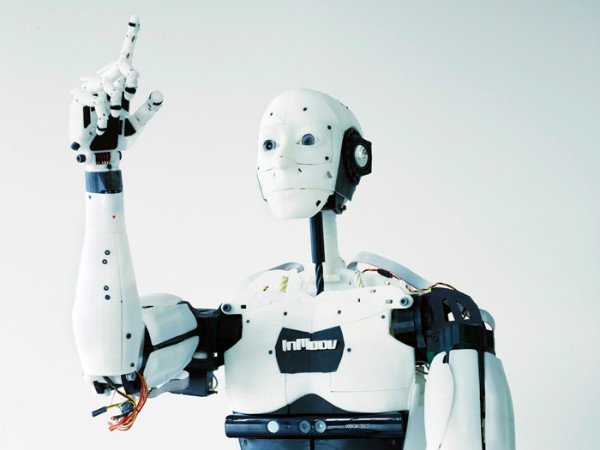
\includegraphics[scale=0.5]{images/Inmoov.jpg}
  \caption{The original form of the open source humanoid robot InMoov, which is designed by Gael Langevin. Image: Gael Langevin, from Wikipedia.}
  \label{fig:inmoov}
\end{figure}



The design framework was mainly influenced by two research papers which detail design frameworks for social robots \cite{bartneck2004design, huijnen2017implement}, with four articles defining design guidelines for robots used with autistic children acting as secondary influences \cite{designSpaces, giullian2010detailed, michaud2003characteristics, robins2007eliciting}.

\begin{figure}
\centering
  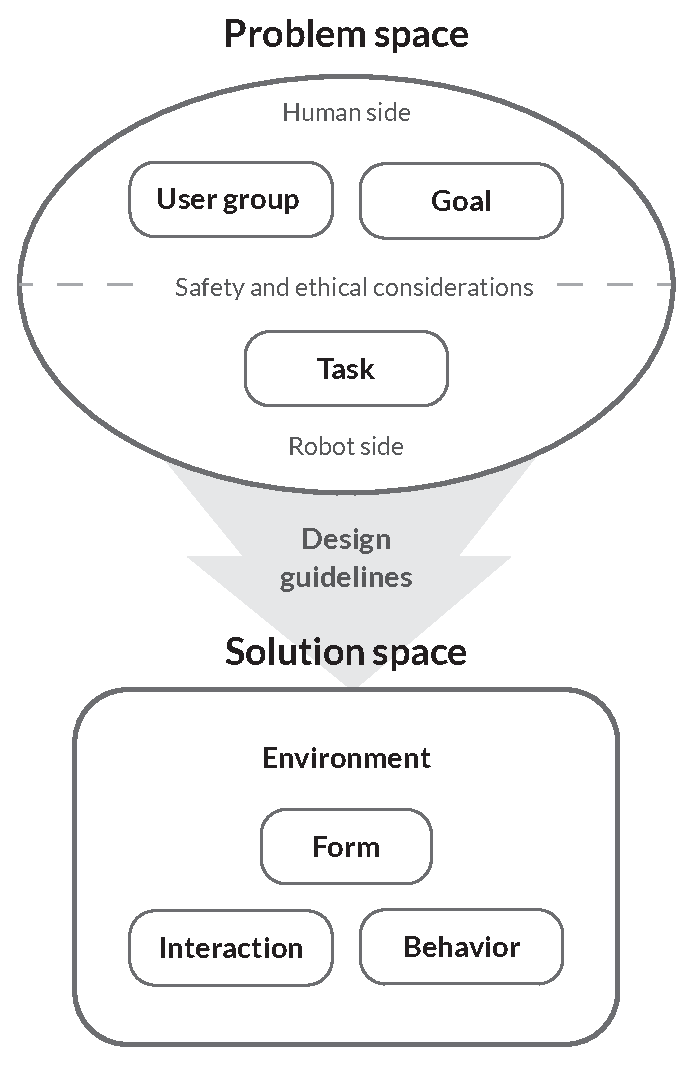
\includegraphics[scale=0.65]{images/designframework_v3.pdf}
  \caption{A proposed framework for the design of social robots. The design framework shows an abstraction of the process of design: first defining the problem space, then the design guidelines that emerge from that specific problem space, and the resulting solution space.}
  \label{fig:designframework}
\end{figure}

Huijnen implemented a co-creation design framework specifically for the design of robotic interventions for children with autism. The primary design dimensions which Huijnen describes are ``robot'', ``end-user'', ``environment'' and ``practical implementation'', which lead to a ``new intervention'' when defined \cite{huijnen2017implement}. Bartneck defined a design framework with five parameters: ``form'', ``modality'', ``social norms'', ``autonomy'' and ``interactivity''. Each parameter is rated along a scale, for example ``form'' ranges from abstract, to bimorphic, to anthropomoprhic \cite{bartneck2004design}. 

The structure of Huijnen's ``process'' was used to inspire the framework presented here. Huijnen first defined four dimensions, which led to the development of the new intervention \cite{huijnen2017implement}. Bartneck's idea of design parameters rated on ranges was incorporated into the design framework presented here \cite{bartneck2004design}. Additionally, four articles discussing the design requirements for robots to be used for autistic children specifically were examined for common design dimensions, although they were not explicitly mentioned in the articles \cite{designSpaces, giullian2010detailed, michaud2003characteristics, robins2007eliciting}.

The influence of these articles led to the realization of the process and design dimensions described in the framework presented here (figure \ref{fig:designframework}). First the design problem space is defined, which involves defining the user group, their goal, and the task of the robot. The problem space was examined already in the previous chapter: the nature of the user group and their issues and goals in therapy were discussed, along with the qualities of previous robots used in these interventions. The solution space is briefly discussed again in this chapter, as it is situated into the design framework. The qualities of the problem space lead to design guidelines, which were defined in the previous chapter. These design guidelines guide the decisions made in the solution space, which is discussed in this chapter. Defining the social robot as a solution involves making design decisions about its form, the way it can interact, and its behavior, which are all affected by the environment the robot is operating in.





\section{Relevant design theory}

The design framework is an abstraction of the design problems related to social robots, and decisions that need to be made when designing social robots in general. While in this thesis it is used for the specific purpose of designing a robot to teach assistive signs to children with autism, it can be used for the design of other social robots.

The design framework presented should be used at the start of the design process. It aids in defining the problem clearly for all individuals involved in the design process, as well as in considering all the dimensions relevant in the design process. The framework itself does not provide methods for granular design, but functions as a primer for considerations about the robot. When designing a robot with an interdisciplinary team, the design framework can be utilized as a boundary object, which helps bring knowledge into a material form, creating conditions for collaboration \cite{nicolini2012understanding}.

The framework describes the entire design process of a social robot, from problem space to solution space. The robot implemented here is used for a pilot study, so its design is a prototype, and is not planned to be the final version of the robot. Performing pilot studies with prototypes provides the opportunity to make ideas tangible faster, so that they can be evaluated and refined, and the best solution can be found faster \cite{brown2009change}. In use of the framework, after the implementation of the robot, another design iteration should be completed based on the examination of the initial implementation. This is a technique called iterative design, adapted from the design of computer user interfaces. Each iteration should be subjected to user testing or other usability evaluation \cite{nielsen1993iterative}. Iterations should be continued until the user issues have reached an acceptable level, or solved entirely. The iterative process to be used with the design framework for designing social robots is detailed in figure \ref{fig:designIterations}. In the case of this thesis, only one iteration was completed. User feedback is detailed in chapter \ref{chapter:results}, while what would be new design guidelines for the next iteration are discussed chapter \ref{chapter:discussion}.

\begin{figure}
\centering
  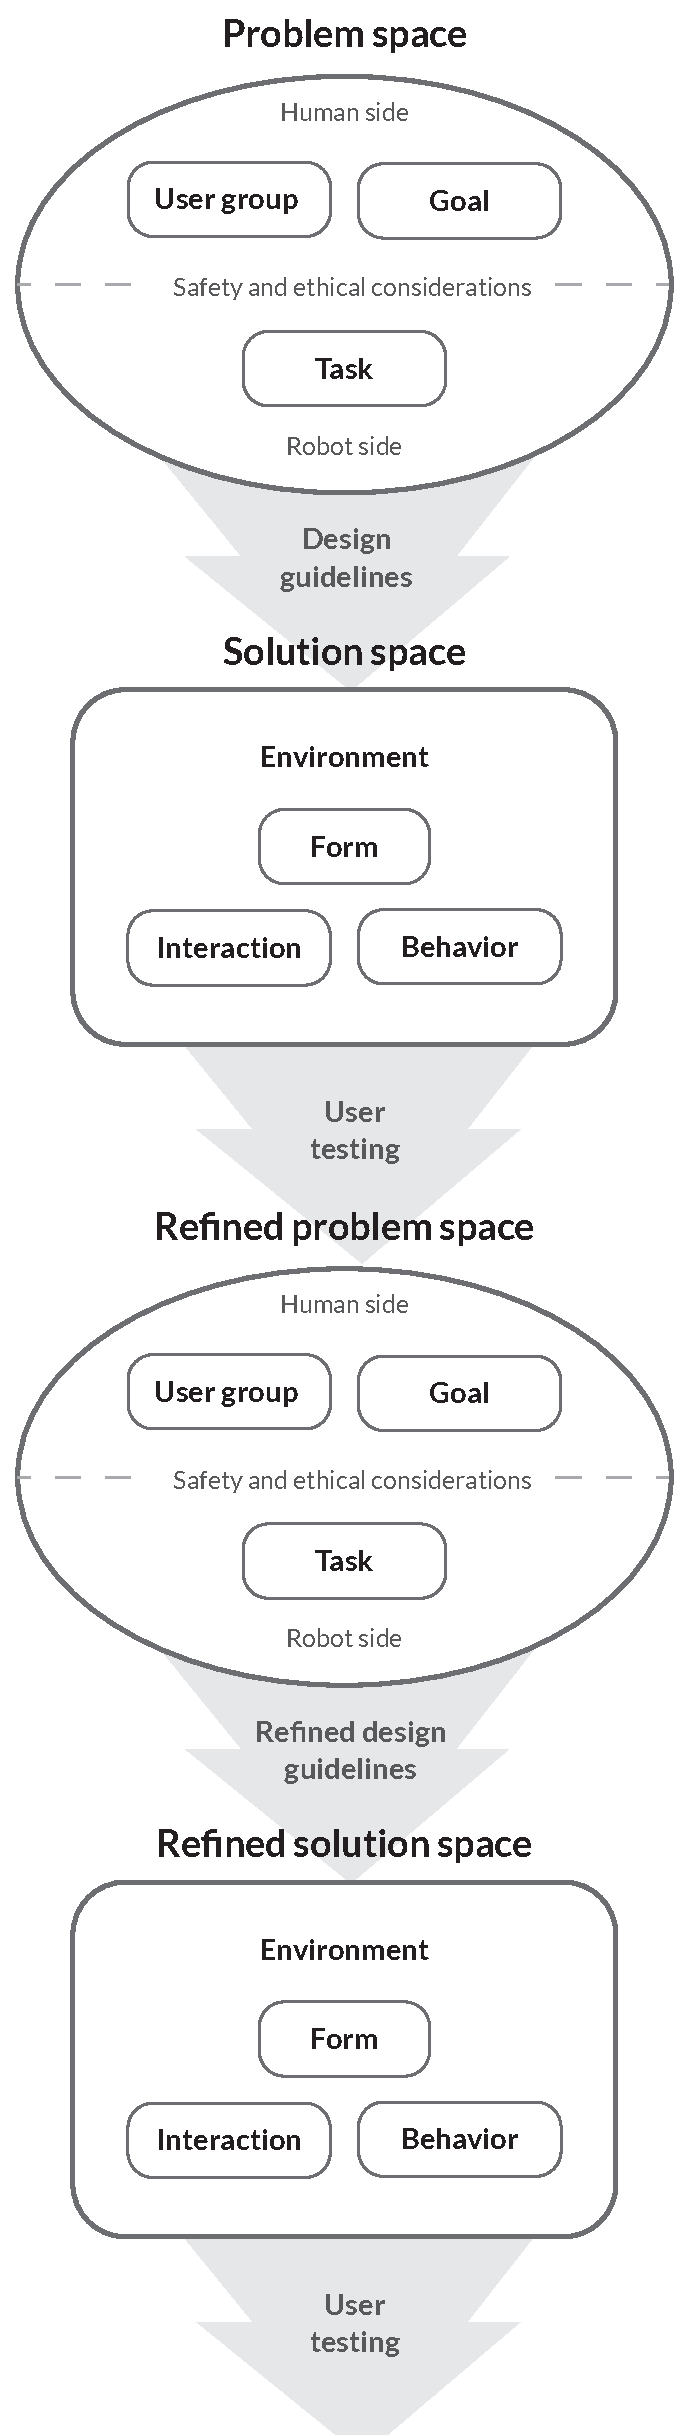
\includegraphics[scale=0.35]{images/design_iterations.pdf}
  \caption{The iterative design process to be utilized with the social robot design framework. After initial definition of the problem space, design guidelines and solution space, a round of user testing should take place. User testing evaluates the proposed solution, after which changes should be made. User testing could reveal that the original user group or their goal, the robot's task, or safety and ethical considerations were not adequately defined or constrained, which is why they should be re-examined after user testing. New design guidelines for the next iteration should be defined, and any existing design guidelines from the previous iteration that were not yet fully realized should be kept. The solution space should be refined and altered based on the user feedback.}
  \label{fig:designIterations}
\end{figure}


Designing social robots requires a deep understanding of human behavior and intelligence, in order to build their behavior in a way that seems intuitive to humans. Specifically, interdisciplinary knowledge and co-operation are needed, to build robots and applications that play a beneficial role in people's lives. Breazeal details a multidisciplinary approach where ``the design of social robot technologies and methodologies are informed by robotics, artificial intelligence, psychology, neuroscience, human factors, design, anthropology, and more.'' \cite{Breazeal2008}

As Breazeal recommends interdisciplinary collaboration, experts in the field of treating autism were consulted for the design of this robot. Designing the InMoov for use as an assistive sign teacher for autistic children involved two experts from the Satakunta hospital district, where the experiments would be performed. These experts were consulted during the definition of the dimensions of the robot in this design framework. Terhi Nyman is a psychologist specialized in neuropsychology, and the psychologist in-charge of social services at Satakunta's health care district. She has worked with people with autism and developmental disorders for over 10 years, and is well versed in the diagnosis and rehabilitation of ASDs and developmental disorders. Akuliina Lehtonen is a speech therapist who has been providing speech therapy for two years, and has over 10 years of experience of working with people with developmental and speech disorders. 

Knowledge of the experts was gathered during collaborative conversations where initial design decisions about the robot were made. Additionally, the speech therapist examined the robot and gave final suggestions before experiments were performed. Electronic communications were also utilized with both Lehtonen and Nyman to obtain additional knowledge. In this design process, new knowledge was created through the interaction between the tacit knowledge of the experts – which is converted into explicit knowledge through collaboration – and the explicit knowledge gathered from the theoretical research. This method of knowledge creation has been  described by Nonaka \cite{nonaka1995knowledge}. In the future, the knowledge of these experts should be captured by using the presented design framework as a boundary object of collaboration \cite{nicolini2012understanding}. By doing this, the experts will act more as participants in a co-design process, rather than external consultants. Experts should be involved in each design iteration. 


%%%%%%%%%%
%%%%%%%%%%
 
\section{Problem space}

Examining the problem space of designing a social robot involves defining the human side and the robot side of the problem (visible in figure \ref{fig:designframework}). Guiding the interaction between the two are safety and ethical considerations. These must be an integral part of any proposed solution, and so they must be discussed already during the definition of the problem.

\begin{figure}
\centering
  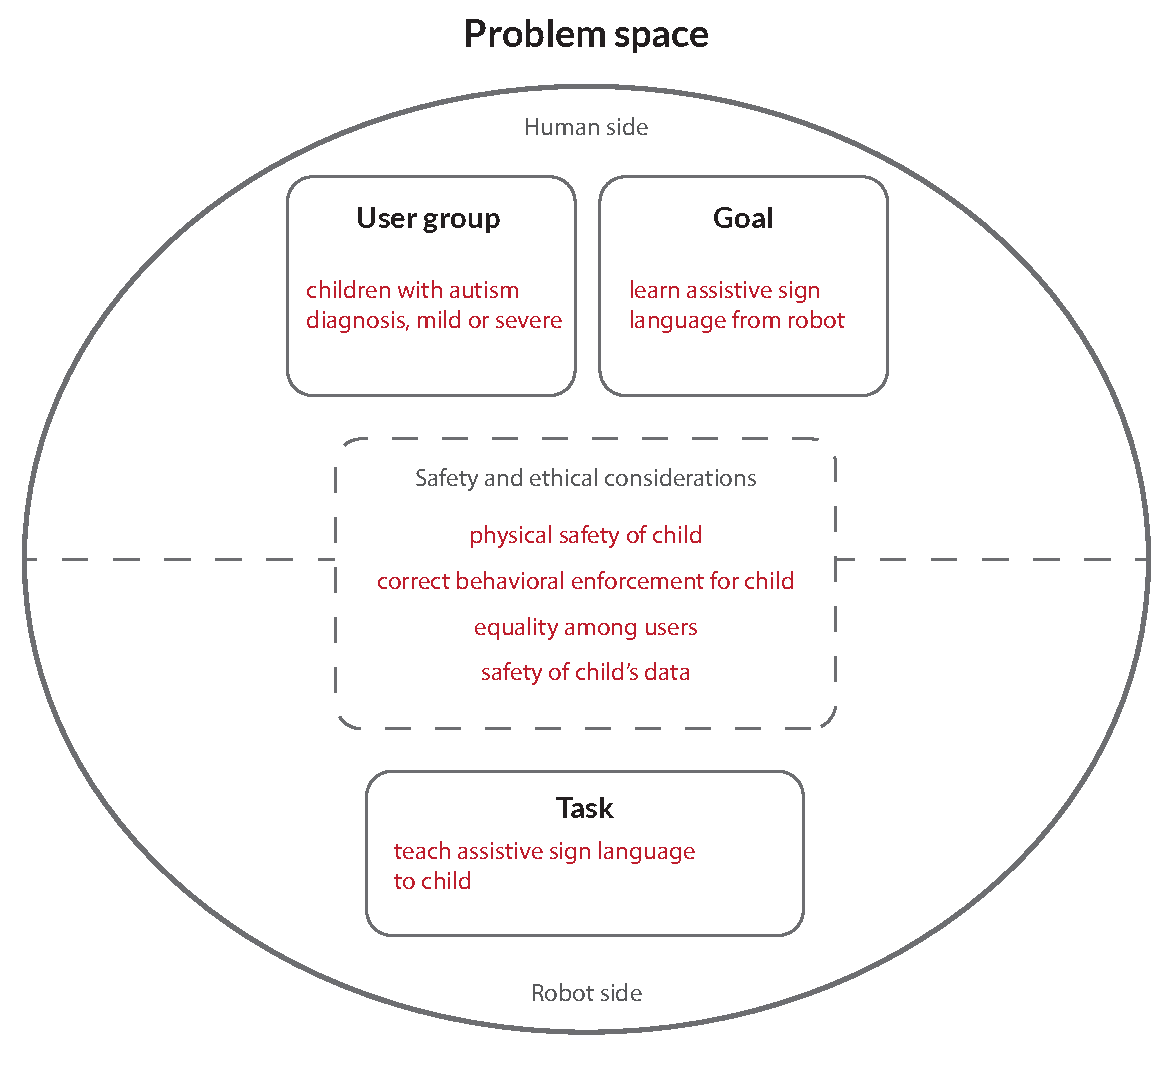
\includegraphics[scale=0.65]{images/problem_v1.pdf}
  \caption{The problem space of designing a social robot encompasses the user group, the user's goal, and the robot's task. Between the interactions of these two operators, safety and ethical considerations emerge.}
  \label{fig:problem}
\end{figure}




\subsection{User group}

On the human side, defining the user group is the first step toward defining the problem space. Defining a user group is important, in order to perform analysis on it and define what it needs. The user group is usually a specific demographic, with specific characteristics, whose needs and interests are steered by those characteristics. 

In this case, the user group is children with a diagnosis of either mild or severe autism (figure \ref{fig:problem}). The child should have the skill to recognize objects from photos, since this will be used with the robot as well. The child also should not have severe degradation of motor skills, so that they have the ability to learn signs. While children are different and have different preferences, some generalizations can be made based on the user group to design a starting point for the robot. 



\subsection{Goal}

After defining the user group, their goal is defined. A clearly defined goal helps examine the eventual solution's success, by whether it accomplished the defined goal for the user or not. The goal is specific to a user group, and should be thought of in terms of short-term and long-term goals.

In the case of autism therapy, therapeutic tools should have designs that have the goal of creating therapeutic value and meeting the individual, social and cognitive needs of the children involved in therapy \cite{designSpaces}. The goal for the users in this solution is to learn assistive signs from the robot (figure \ref{fig:problem}). The long-term goal would be for children to learn the signs on such a level that they are able to incorporate them into use in their daily lives. The short-term goal of the children is to successfully imitate the robot during the experiments. 


\subsection{Safety and ethical considerations}


Roboethics was a field established in 2004, which focuses on the human ethics of the robots' designers, manufacturers and users (instead of the robot and its artifical ethics). Roboethics are realized in the interaction between the robot and its user  \cite{Veruggio2008}. Safety and ethical considerations are important, as users may not always be aware of the potential negative consequences of using technology, and should be protected from negative effects by the designers of the robot.

In this design framework, safety and ethical considerations are realized on the border between the human side and the robot side (figure \ref{fig:designframework}). Safety and ethical considerations guide the definition of the problem space, and affect the design in the solution space. The safety and ethical treatment of both the user and their data should be taken into account. In this case, four considerations for the safety and ethical treatment of the user were defined for this robot-mediated intervention (figure \ref{fig:problem}). The implementation of these considerations is discussed in chapter \ref{chapter:solution}.

The physical safety of the child needs to be ensured while using the robot \cite{giullian2010detailed}. Machinery has the potential to crush or pinch the user if operated recklessly. 

Correct behavioral enforcement for the child was discussed with the psychologist and speech therapist. This means that the robot should not intend to replace human contact for the child, but to act as a tool to supplement learning. Mistreatment of the robot by the child should also be intervened in, so that the child learns that that behavior is not acceptable. Children have shown potential to treat social robots in an abusive manner when unsupervised \cite{brscic2015escaping}. Bad behavior toward social robots may even begin influencing children's behavior toward humans \cite{walk2016}. In this case, behavioral interventions were decided to be done by the human working with the child and the robot, rather than by the robot itself. Rewarding of the child when they behave correctly was also defined to be important for learning correct behavior.

Equality of the users was also discussed with the professionals. While the majority of children with autism diagnoses are boys, the number of female autism diagnoses has been steadily rising, faster than male diagnoses \cite{jensen2014time}. It has been argued that the lower number of female diagnoses is due to women being underdiagnosed with autism \cite{krahn2012extreme}. It has also been argued that males are generally more likely to be autists, as autism is a presentation of an ``extreme male brain'' \cite{baron2002extreme}. Due to disagreement on this matter, it was decided to keep the robot neutral in gender representation.

Data collected from experimental participants should be kept safely, especially in a medical context, in order to ensure privacy. Robots are in a unique data collection position when compared to personal computers, because they feel more social to humans, and elicit emotional responses \cite{calo2014case}, which may lead to the revelation of more personal data to the robot.  If data is used nefariously, especially sensitive emotional data that can be collected by a robot operating in a therapeutic context, there is potential for manipulation. It should be carefully considered what is an appropriate trade-off for users giving their data, and receiving a benefit from the processing of that data \cite{darling2015s}. In this case, the robot did not record any data, but data collected from the experiments was treated with the same respect.



\subsection{Task}

On the robot's side of the problem space, the robot's task is defined. The task is directly related to the user's goal. The task is the primary purpose for which the robot is built, and is what it needs to accomplish with the user. The build of the robot is completed once it can successfully accomplish the task. The task should also be thought of as both long-term and short-term.

In this case, the long-term task is teaching assistive sign language to the child. The short-term task is to produce the pre-defined signs accurately, and to respond to the child's behavior appropriately.


%%%%%%%%%%
%%%%%%%%%%


\section{Solution space}

\label{chapter:solution}

 \begin{figure}
 \centering
  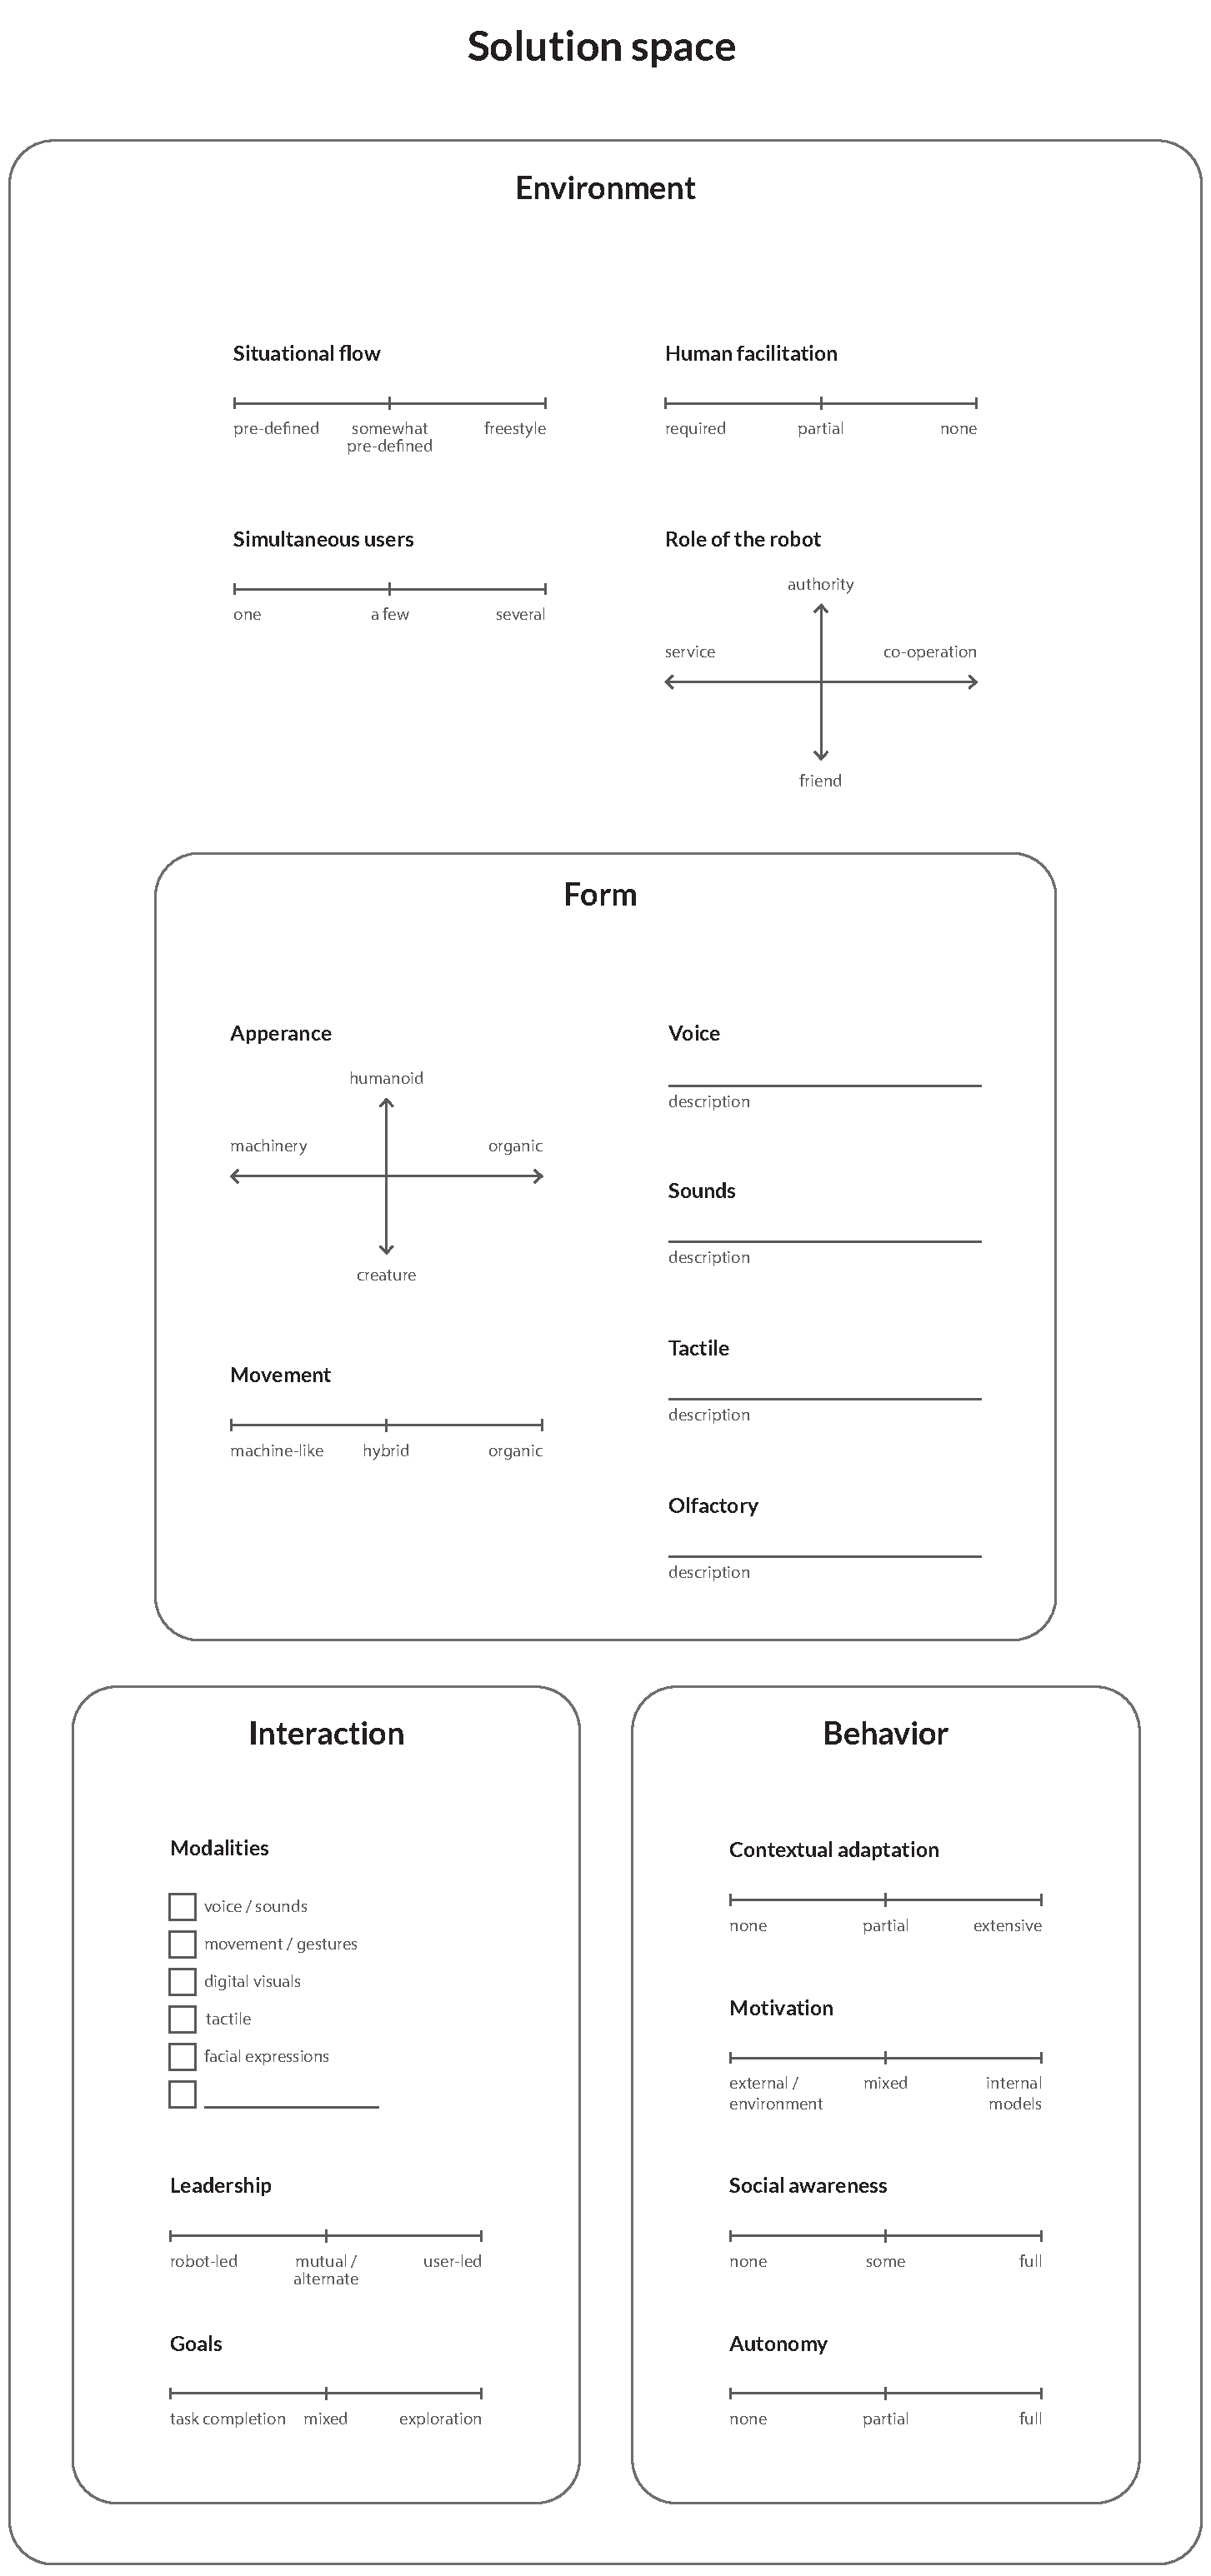
\includegraphics[scale=0.4]{images/solution_v4-01.pdf}
  \caption{Detailed depiction of the solution space in the framework for designing social robots. Defining the solution space involves designing the robot's environment, form, interaction and behaviors.}
  \label{fig:solution}
\end{figure}

The design of the solution space is guided by the design guidelines defined in the previous chapter, which were influenced by defining the problem space. Defining the solution space involves making decisions about the environment the robot operates in, which guides decisions made about its form, interaction and behavior (figure \ref{fig:solution}). In reality, these dimensions overlap each other, but this framework aims to make the interlinked decisions apparent and explicit.

The design guideline ``simple form'' specifically guides the form dimension, ``positive, supportive, rewarding experience and environment'' specifically guides the environment dimension, and ``consistent, structured, simple behavior'' specifically guides the behavior dimension. However, all these guidelines should be taken into consideration while designing other dimensions as well, as in reality the dimensions overlap each other. 

The guidelines ``modular complexity'' and ``modular specific to child's preferences'' can be realized in all dimensions. In this thesis, these two guidelines are specifically explored in the interaction dimension, and not touched on in the other dimensions. This is further explained in chapter \ref{chapter:interaction}. In a fully functional clinical solution, these two design guidelines should be realized in all dimensions.

In this case, the robot InMoov was chosen as the platform for the solution, due to availability. The selection of the InMoov creates some pre-defined constraints for the design of its form and interaction. Some of the pre-defined form and interaction qualities of the original InMoov are modified for this implementation. To modify the robot's form, its voice and sounds were modified from pre-set settings. To modify interaction qualities, new hands were added to give better signing ability, a tablet was attached to its chest, and lights were attached to one of its hands. These modifications are discussed in more detail below. Environment and behavior could be freely designed due to not being significantly limited by the InMoov.

First, the dimensions of the solution space are explained on a general level. Then, pre-defined constraints of the design defined by the InMoov are discussed. After this, the specific design for this solution, including modifications, is described. 


\subsection{Environment}

\label{chapter:environment}
\label{sec:environments}

In this framework the environment does not mean the location of the robot, but rather all factors surrounding its operation. The environment is examined through four qualities: situational flow, simultaneous users, human facilitation and role of the robot, as seen in figure \ref{fig:environment}. The design driver ``positive, supportive, rewarding experience and environment'' guides the design of this dimension. 


 \begin{figure}
  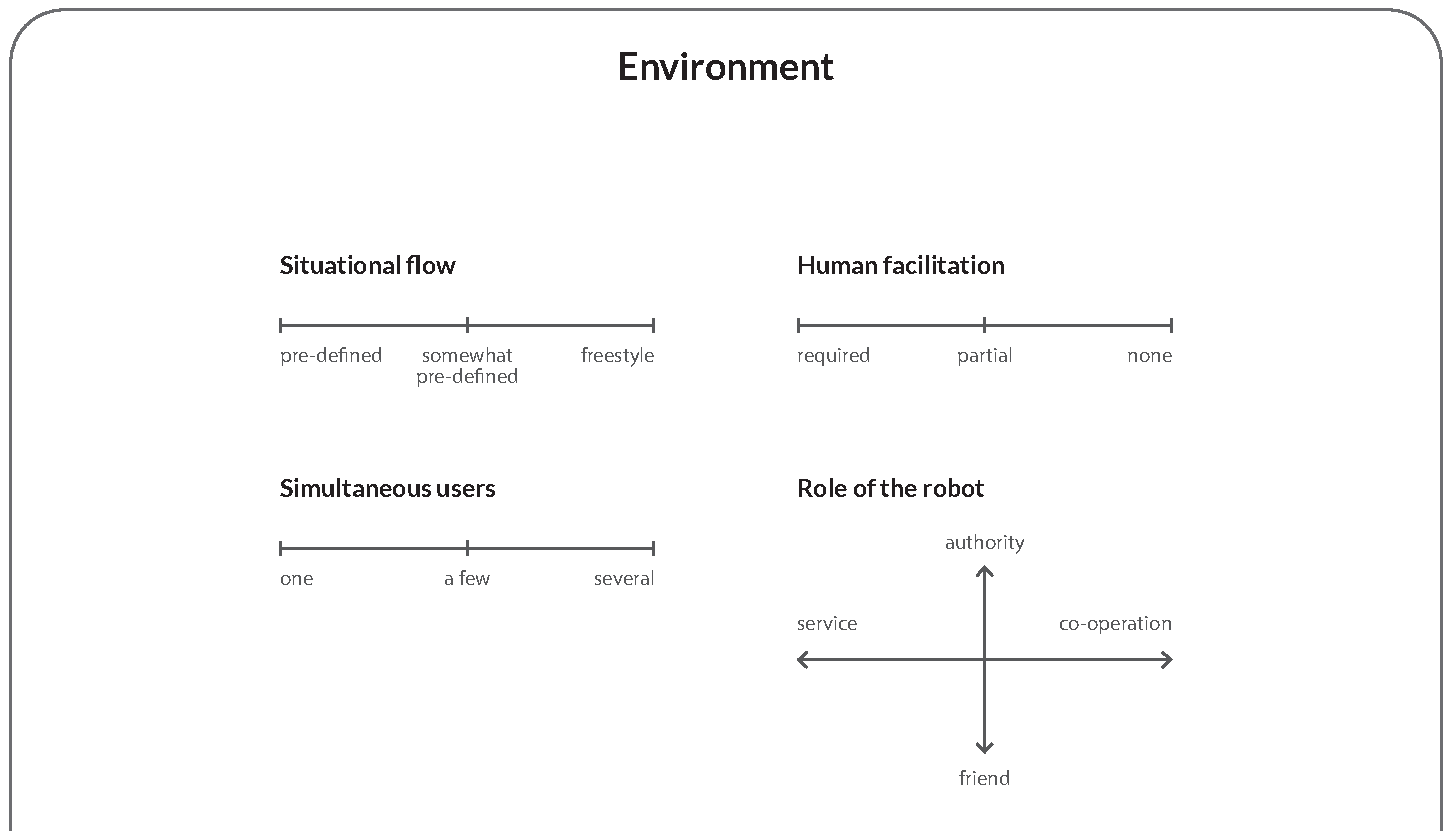
\includegraphics[width=\linewidth]{images/solution_v4-02.pdf}
  \caption{Defining the environment of the social robot involves examining the nature of the situational flow of the interaction with the robot, and the step preceding and following it. It also involves making decisions about the number of simultaneous users, the level of human facilitation needed in the solution, and the nature of the role of the robot in its environment. The environment affects design decisions made of the robot's form, interactions and behavior.}
  \label{fig:environment}
\end{figure}

The design choices made for the environment of the solution in this case can be seen in figure \ref{fig:environmentFinal}.


\begin{figure}
  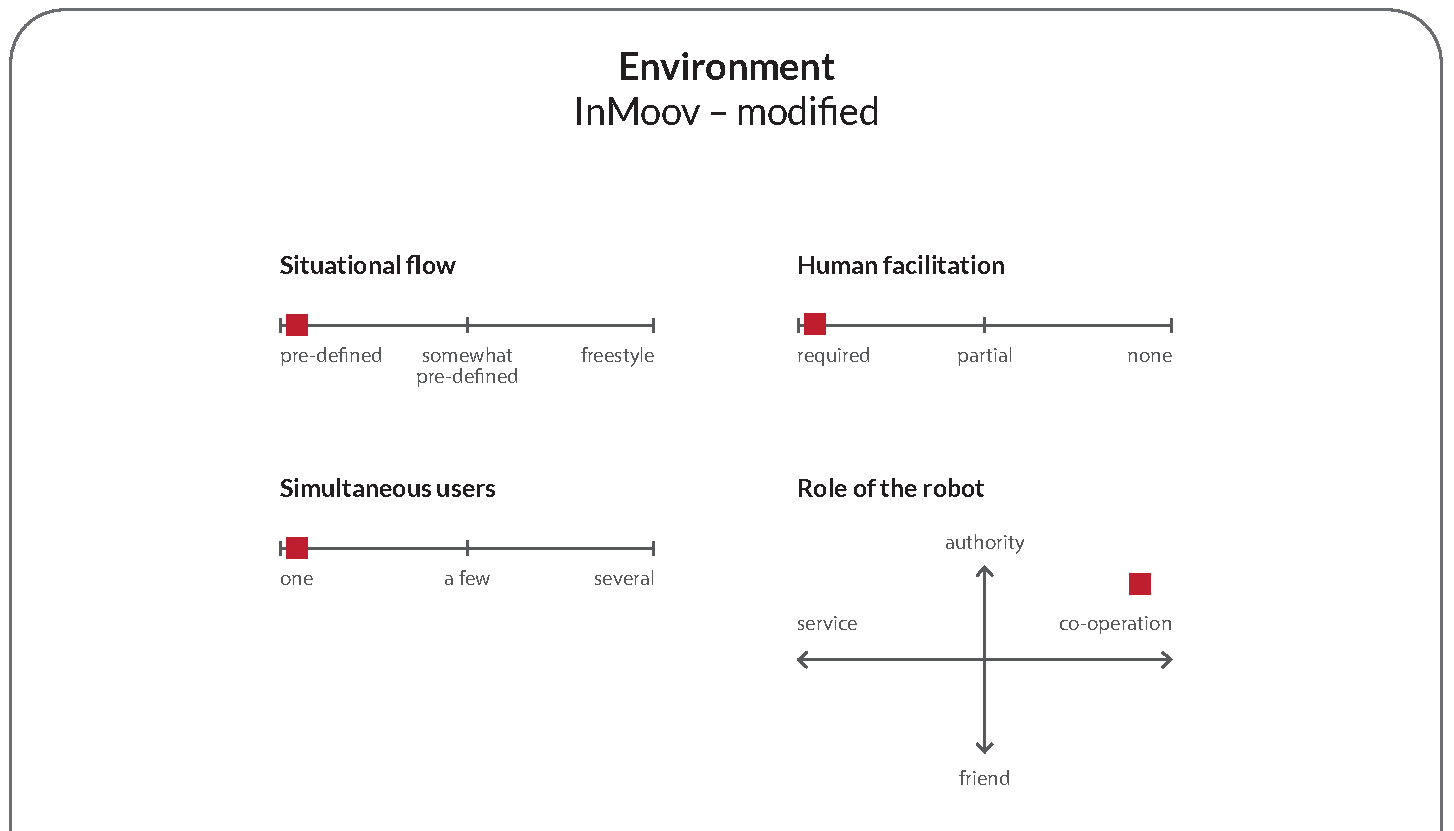
\includegraphics[width=\linewidth]{images/solution_inmoov_final-02.pdf}
  \caption{Design choices made about the environment of the solution provided with the InMoov, shown in red.}
  \label{fig:environmentFinal}
\end{figure}


\subsubsection{Situational flow}

The situational flow describes how pre-defined the environment surrounding the interaction with the robot are, ranging from pre-defined, to somewhat defined, to freestyle. Situational flow describes how exactly the events leading up to and after the interaction with the robot are defined.

The situational flow of this solution is highly pre-defined, as seen in figure \ref{fig:environmentFinal}. What happens before and after the therapy situation is rigidly pre-defined, since people with autism prefer routine and unexpected situations may upset them \cite{frith2003autism, tetzchner}. The child is accompanied by their companion and the speech therapist when going into and out of the room, in order to support them during what may be a stressful experience. The exact experimental procedure is detailed in chapter \ref{chapter:methods}. This follows the ``positive, supportive, rewarding experience and environment'' design guideline.


\subsubsection{Simultaneous users}

Simultaneous users describes how many users interact with the robot simultaneously in the environment.

In this case, there is only one user, due to the pilot nature of the study. This thesis aims to observe the direct interaction between one child and the robot. In future interventions, children could potentially interact with the robot and another child, or another person. This would require re-designing the environment of the robot accordingly.


\subsubsection{Human facilitation}

The level of human facilitation of the environment describes whether the interaction between the robot and the user needs another human's support to move forward. If the robot is part of a chain of events in which humans are involved, human facilitation is required. If the robot freely exists in a space, with users free to interact with it as they please, there is no human facilitation. Partial human facilitation can for example mean a designated human guiding users toward the robot.

The use of a robot in this context needs human facilitation. The child should not be alone with the robot due to safety and ethical concerns discussed in the problem space: physical safety of the child and correct behavior reinforcement. To ensure the physical safety of the child, the robot has a quickly activated stop button in case of emergencies, as recommended \cite{giullian2010detailed}. However, intervention by a human facilitator is the primary way of preventing the child from getting too close to the robot and injuring themselves. The presence of another human also ensures correct behavioral reinforcement, by ensuring that the robot does not replace human contact, and by intervening if the child were to mistreat the robot. 

The operation of the robot from the control room is made easier with a human facilitator. The human facilitator, in this case the speech therapist, signals to the operator how the robot should behave. A companion of the child, meaning a parent or other caretaker, is also present in the therapy to help the child feel safe and calm. This follows the ``positive, supportive, rewarding experience and environment'' design guideline.


\subsubsection{Role of the robot}

The role of a robot is highly variable. Huijnen defines the roles of robots used in autism therapy as ``provoker'', ``reinforcer'', ``trainer'', ``mediator'', ``prompter'', ``diagnoser'', and ``buddy'' \cite{huijnen2017implement}. However, for the general design of social robots, these roles are too few. Because all possible roles can not be listed in a design framework, a two-dimensional map is implemented, within which roles can be situated. There are two ranges, from service to co-operation, and authority to friend. This describes the robot's relationship to the user in the given environment. The robot can either serve the user, or they can co-operate on a task. The robot can act as an authority with the user, maintaining distance, or it can act as a friend, feeling closer to the user. The robot does not have to be strictly one or the other, but can fall into sub-divisions on the map.

In this solution, the robot is an authority for the child. Becoming more of a friend would require physical contact (as with for example Probo, the huggable robot \cite{ProboRef}), which was not possible due to the fragility of the InMoov. The robot being framed as an authority can also help the child focus on the task at hand and follow its instructions, and not on ``making friends'' with the robot. 

The robot is more of a co-operator than a server. The robot and the child take turns signing, thus working together, rather than the robot performing a task for the child.

To create a supportive and rewarding experience as a co-operating authority, the robot should reward the child when they sign correctly. If the child signs incorrectly or does not react, however, the robot is not critical, and is supportive of the child. This follows the ``positive, supportive, rewarding experience and environment'' design guideline.


\subsection{Form}

\label{chapter:form}

The form of the robot encompasses all its externally perceptible qualities. Defining the form of the robot involves examining six qualities: appearance, movement, voice, sounds, tactile sensations and olfactory sensations, as seen in figure \ref{fig:form}. ``Simple form'' is the primary design guideline of this solution dimension.

\begin{figure}
  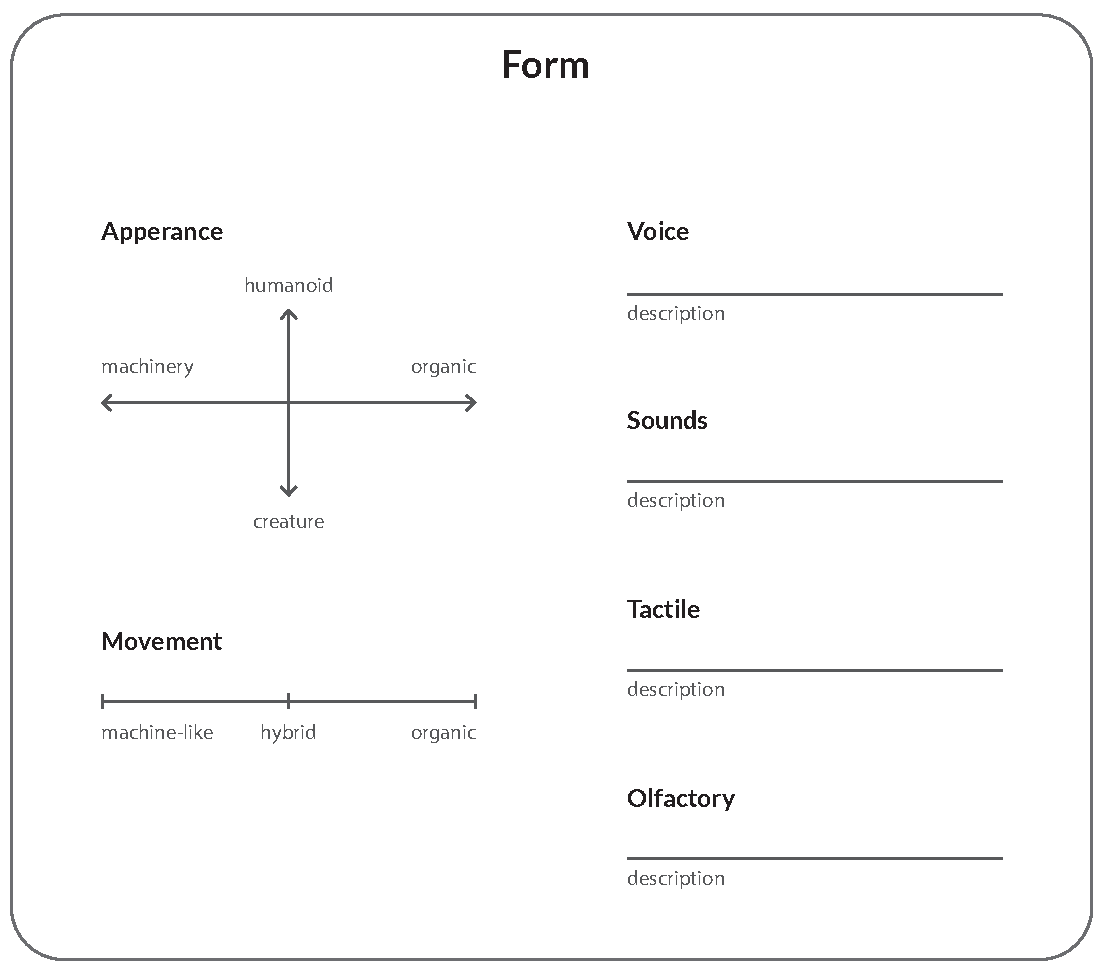
\includegraphics[width=\linewidth]{images/solution_v4-03.pdf}
  \caption{Defining the form of a social robot involves making decisions about its appearance, the way it moves, its voice and sounds, and tactile and olfactory sensations. As voice, sounds, tactile and olfactory sensations are all highly variable, freeform descriptions are used.}
  \label{fig:form}
\end{figure}

A well-known measure of a robot's form in the field of robotics is evaluating the robot according to its ``familiarity'' to life. This is defined by the degree to which the robot resembles human-like appearance and movements. It is argued that a robot should not be too human-like, or it will fall into the ``uncanny valley" of negative familiarity, appearing like an animated corpse. The original theory of the ``uncanny valley" suggests that a robot should not be made to be too human-like, as a safe familiarity can be produced by a design approaching human likeness, but not too close to it \cite{mori1970uncanny}. This theory can be further expanded into creature-like robots: they should not be made too life-like, to avoid appearing zombie-like. The appropriate degree of familiarity according to this theory is generally accepted in the field of robotics, which is why it is not introduced as a variable in this framework. This accepted level of familiarity – approaching human or creature likeness, but not attempting to be an exact copy – can be achieved by appropriately designing the qualities that make up the robot's form. All dimensions of the robot's form contribute toward its life-likeness, with appearance and movement being most important.

In this case, defining the form of the robot for the solution had some constraints, due to selection of the InMoov as a solution platform. Pre-defined form qualities are visible in figure \ref{fig:formPredefined}. The original form of the InMoov (figure \ref{fig:inmoov}) is used as a base, and modified according to the established design guidelines, and safety and ethical considerations. The modifications done to the InMoov's form can be seen in figure \ref{fig:formFinal}. The open source nature of the InMoov makes modifying it possible. Modifying the robot's voice and sounds is possible through its open source MyRobotLab software.


\begin{figure}[htbp]
  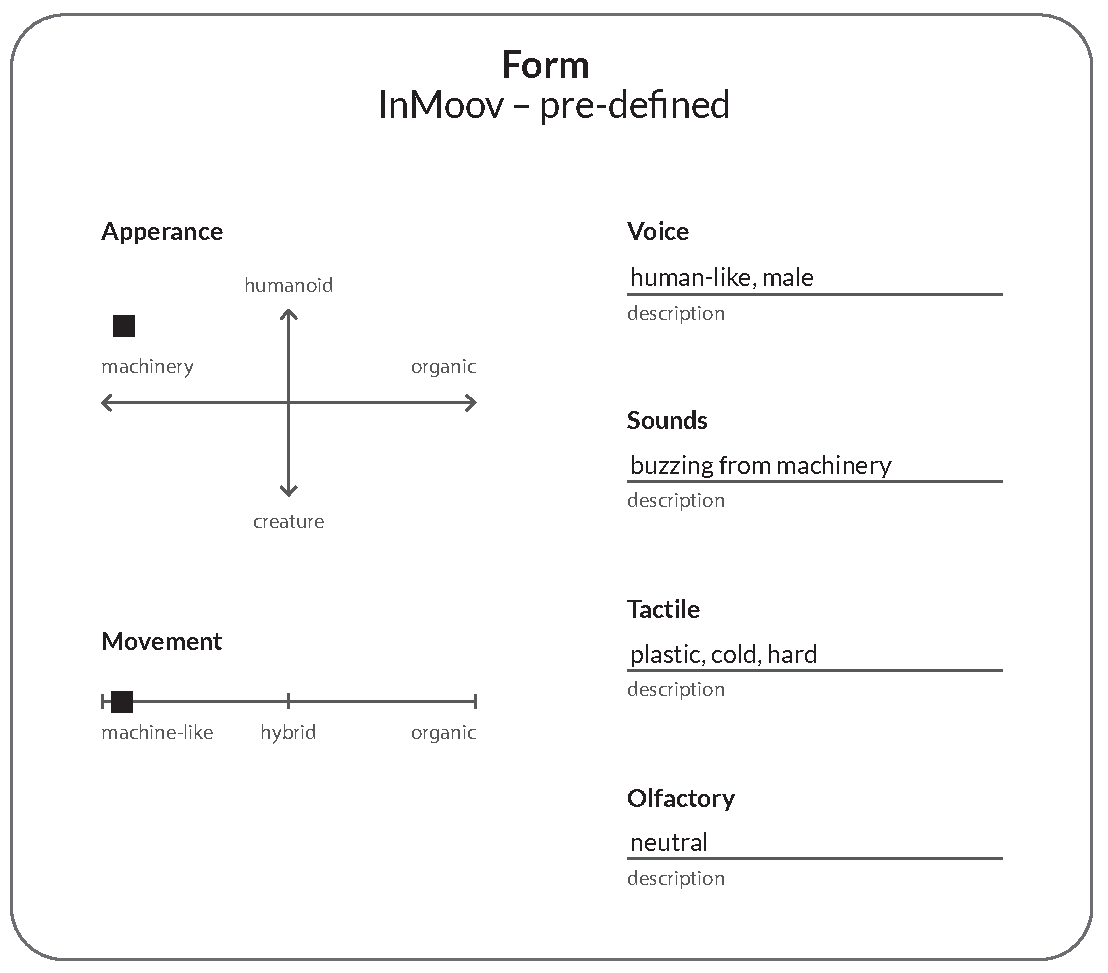
\includegraphics[width=\linewidth]{images/solution_inmoov_predefined-02.pdf}
  \caption{The choice of InMoov as the solution platform set the baseline for form design.}
  \label{fig:formPredefined}
\end{figure}


\begin{figure}
  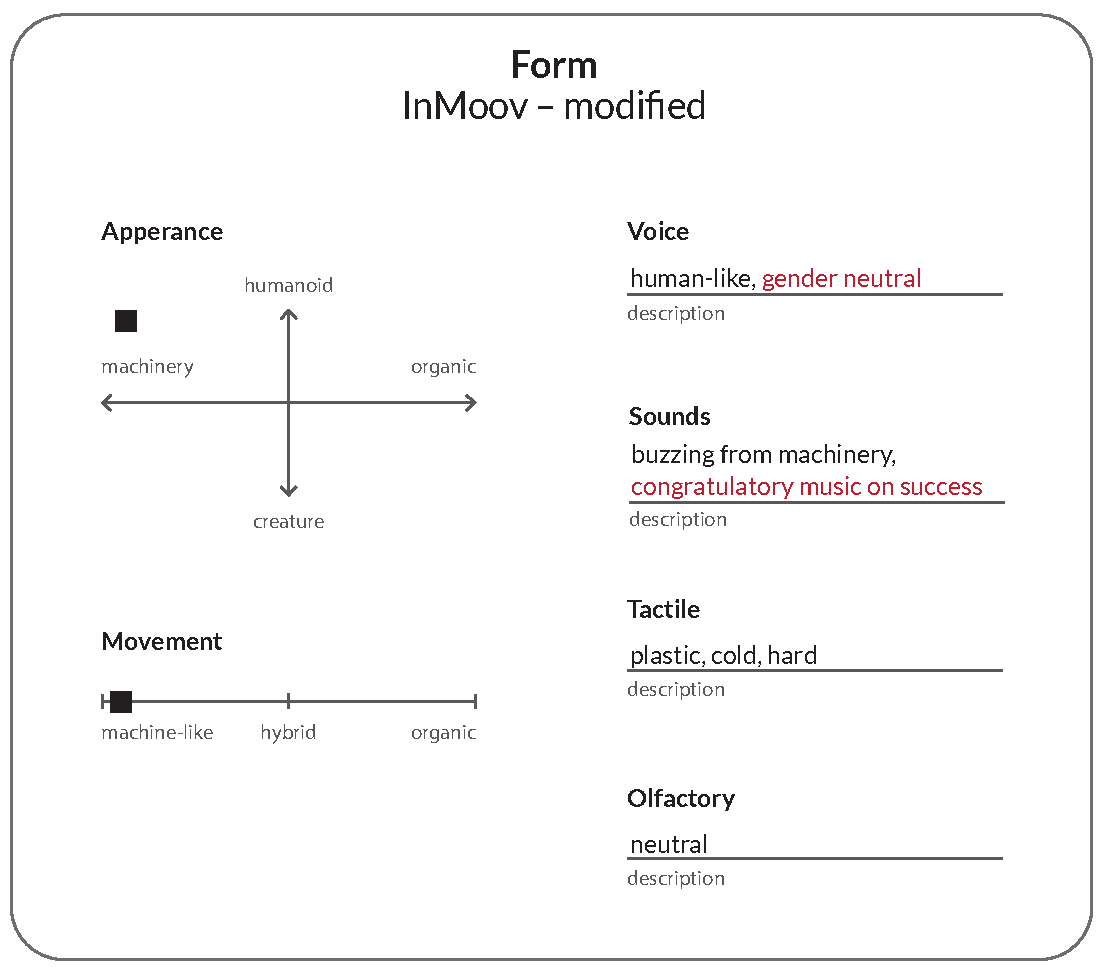
\includegraphics[width=\linewidth]{images/solution_inmoov_final-03.pdf}
  \caption{The design baseline of the form pre-defined by the InMoov is shown in black, and the modifications made to it are shown in red.}
  \label{fig:formFinal}
\end{figure}


\subsubsection{Appearance}


The appearance of a robot is highly variable, which is why a two-dimensional map is used to describe it. In this framework, the appearance can range from machine-like to organic, and from humanoid to creature-like. The appearance of a robot defines the user's initial response to it. If a robot appears sophisticated, the user will assume similar level of sophistication in its skills \cite{bartneck2004design,designSpaces}. A humanoid robot is perceived as human-like, and elicits strong expectations about the robot's social and cognitive competencies \cite{designSpaces}, while a creature-like robot is perceived as more of an animal, with a lower level of functioning. 

The appearance of the robot was not modified significantly from the base InMoov design. The only modifications to the robot's appearance were done for the sake of interaction, and are discussed in chapter \ref{chapter:interaction}. The humanoid design of the InMoov is suitable for this solution, as the goal is for autistic children to use the humanoid robot to practice skills related to human-to-human communication \cite{designSpaces}. The robot is mechanical in appearance, but not so mechanical that the child would be more interested in examining its components, rather than interacting with it. The robot is easily discernible as humanoid, but also robotic enough to not be confused with a human \cite{giullian2010detailed}.

The InMoov's original face design was also suitable for this solution. The face is simple with distinct features, with no ability for facial expressions. Complex affective expression by human faces have been shown to cause an overstimulation effect in autistic people's brains, which in turn leads to gaze avoidance by the autistic person \cite{dalton2005gaze}. A simple face helps prevent overstimulation, confusion and avoidance \cite{giullian2010detailed}.

The robot was not modified to appear more human, which could have been done with clothing or a wig. This was decided in agreement with the speech therapist and psychologist. This also follows the design guideline of ``simple form''.


\subsubsection{Movement}

In this framework, the movement of a robot can be rated from machine-like, to hybrid, to organic. Organic, smooth movements suggest a more sophisticated robot in terms of skills, while a more mechanical movement quality suggests a more rudimental robot.

It has also been argued that robotic movements, in contrast to human movements, elicit a faster imitation response from autistic children \cite{pierno2008robotic}. However, in this case, the speech therapist recommended that the robot have movements that are as smooth as possible, in order to sign as accurately as possible. The InMoov's base level of movement is machine-like, and difficult to modify. In order to take into account the speech therapist's advice, the InMoov's original hands were replaced with different hands, in order to give the fingers and wrists smoother movements. The robot does not over-extend its limbs, and does not assume positions impossible for humans \cite{giullian2010detailed}.


\subsubsection{Voice and sound}

The robot's voice and the sounds it makes contribute to the robot's life-likeness. A voice can be robotic, or human-like. Voice can be perceived to have a gender or an age, which depends on speed, pitch and other qualities. Voices, both robotic and human-like, can have tonality, being either monotone or having vibrant prosody. The noises a robot can make are almost infinitely variable: machine-like ``beeps", music, human-like exclamations or animal calls are common examples of sounds a robot can make. The sounds that a robot's machinery may make when it moves are also part of its soundscape. A robot's soundscape can also include sounds that it makes when it is touched, or if it is mobile, sounds that it makes when it moves in space.

In this framework, voice and sounds are defined through a free-form description, as they are both highly variable. Measurements via ranges or maps, as are done for the appearance and movement, could be developed in the future, in collaboration with an expert in audio.


The original voice of the InMoov was a human-like male, as seen in figure \ref{fig:formPredefined}. It was decided that the robot should keep a human-like voice, in order to make it more natural to practice human-to-human interaction with. Due to the decision to keep the robot gender-neutral, which was discussed in the definition of the problem space, its voice was modified. A female Finnish-speaking human-like voice, Satu from Apple, was used. Its pitch was lowered to make it indistinguishable as either a male or female voice. Prosody of the voice is defined by the Satu system, which mimics human-like tonality. The voice of the robot was also slowed by 10 \% from the original Satu voice, to make it more understandable to the children.

The robot plays a short congratulatory musical tune through its mouth speaker when a child signs successfully. This provides a sensory reward for the child \cite{robins2007eliciting, michaud2003characteristics}, which follows the design guideline of ``positive, supportive, rewarding experience and environment". 

The InMoov's machinery is quite noisy, and gives off a buzzing sound as it moves its hands. The InMoov's material does not give off sound when touched. The InMoov as a whole is fixed in place, and thus there are no sounds resulting from the robot moving from point to point.


\subsubsection{Tactile sensations}

Tactile sensations are especially important if the user is in close contact with the robot. Soft and warm tactile sensations suggest comfort and familiarity, while hard and cold tactile sensations suggest distance and industrial qualities.

In this framework, free-form descriptions are used to describe tactile sensations, as they are highly variable. In the future, measurements such as ranges or maps could be developed to describe these qualities.

In this solution, tactile properties were pre-defined by the choice of using InMoov as a solution platform. The material used to construct the InMoov is a cold, hard plastic, which suggests distance. However, as the planned interactions with the robot do not include touching it, tactile sensations do not need to be taken into account or modified.


\subsubsection{Olfactory sensations}

Olfactory sensations are also especially important if the user is in close contact with the robot. Olfactory sensations can induce sensations of pleasure or disgust, or they can be entirely neutral.

In this framework, olfactory sensations are defined through a free-form description, as they are highly variable. In the future, ranges or maps could be developed to describe these sensations. 

The olfactory sensations are pre-defined by the InMoov's material, as plastic has no smell and is thus neutral. In this case, there was no need to modify the sensations, as users would not be in close contact with the robot, and could not smell it. 


\subsection{Interaction}

\label{chapter:interaction}

The interaction dimension defines the manner in which a user can interact with a robot. In this framework, interaction is examined through three qualities: modalities, leadership, and goals (figure \ref{fig:interaction}). 

\begin{figure}
\centering
  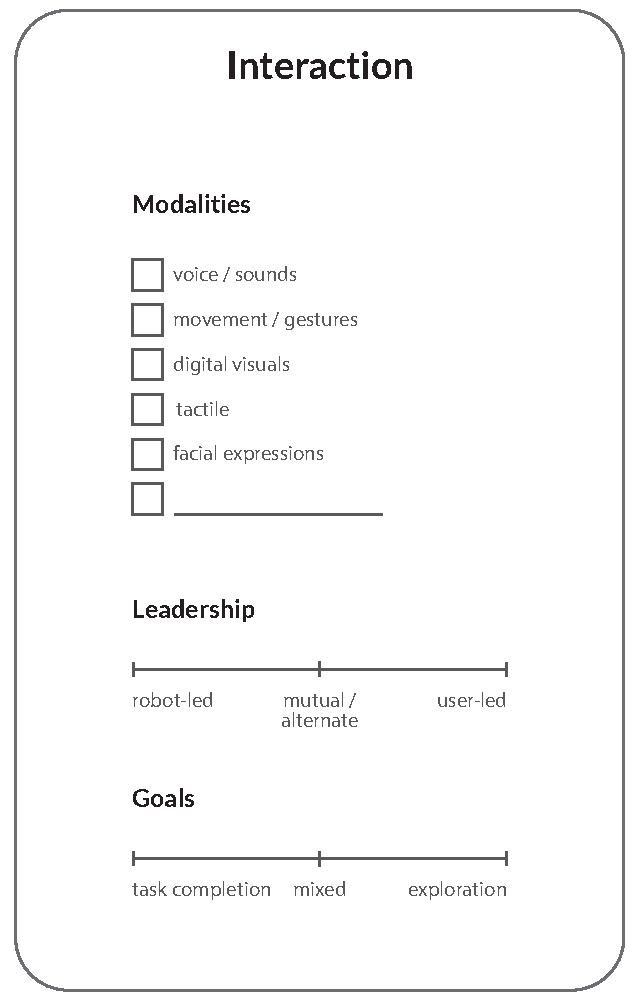
\includegraphics[scale=0.75]{images/solution_v4-04.pdf}
  \caption{The interaction design dimension contains interaction modalities, which can be expanded upon from the list available, leadership of the interactions, and the robot's goals in performing the interactions.}
  \label{fig:interaction}
\end{figure}

No design guidelines defined in the previous chapter specifically guide the interaction dimension. However, the design guidelines ``modular complexity" and ``modular specific to child's preferences" can both be realized in the design of interactions. 

In this thesis, different modalities of interaction are compared. These modalities are used to examine modularity of the robot. In the future, modular qualities of the robot can be used to fulfill the design guidelines of ``modular complexity" and ``modular specific to child's preferences". Due to the pilot nature of this study, these design guidelines are not yet fully realized.

Due to the overlapping nature of the design dimensions, interaction is somewhat pre-defined by the form of the robot. Interacting with the InMoov involves the modalities of voice and gestures, due to the design of the robot's form. The pre-defined interaction qualities are visible in figure \ref{fig:interactionPredefined}, and modifications made to the interaction dimension are seen in figure \ref{fig:interactionFinal}.


\begin{figure}
\centering
  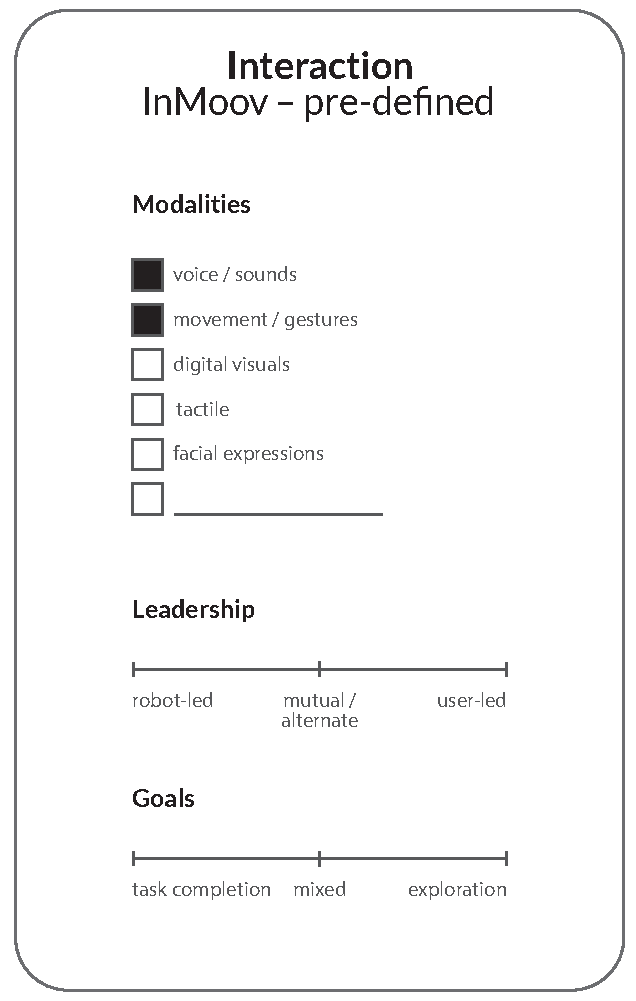
\includegraphics[scale=0.75]{images/solution_inmoov_predefined-03.pdf}
  \caption{InMoov has the pre-set interactions modalities of voice and sounds, and movement and gestures, which set the baseline for design.}
  \label{fig:interactionPredefined}
\end{figure}

\begin{figure}
\centering
  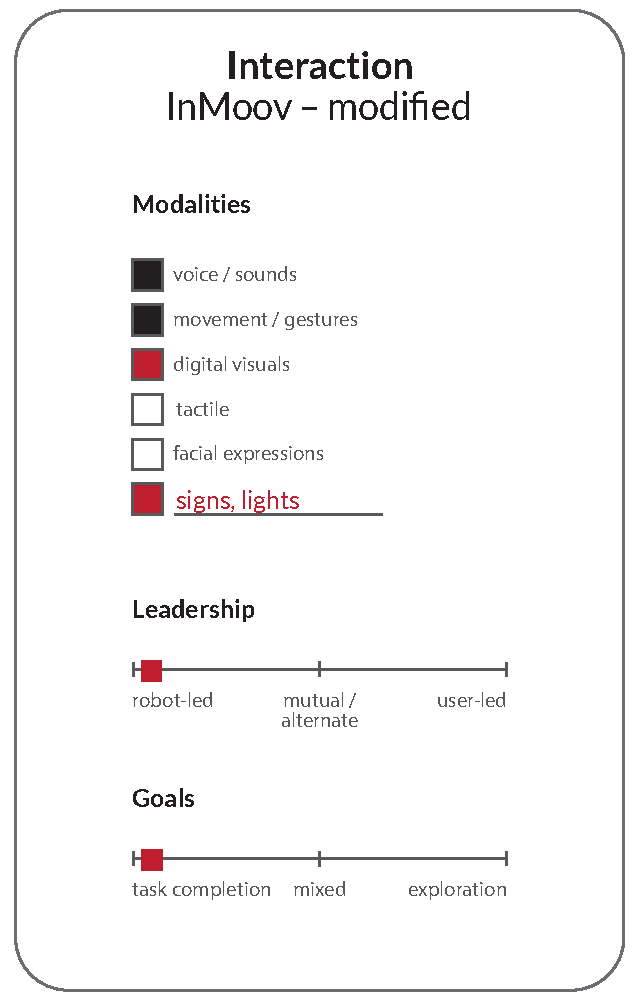
\includegraphics[scale=0.75]{images/solution_inmoov_final-04.pdf}
  \caption{The design baseline for interactions pre-defined by the InMoov are shown in black, and the additions made to it are shown in red.}
  \label{fig:interactionFinal}
\end{figure}



\subsubsection{Modalities}

Modalities of interaction define the different ways a user can interact and communicate with the robot. Modalities of interaction can vary greatly. A list of the most common modalities encountered in interaction with robots are listed in this framework. Additionally, an empty space for novel modalities is provided. Modalities are restricted by what human senses can perceive. Even though a robot could theoretically communicate via radio frequency, a human can not do this, so interaction through this modality is not possible. Robots can interact via multiple modalities, either simultaneously or one after the other.

For this solution, interaction modalities were discussed with the psychologist and speech therapist, and determined to be a special area of interest in communication therapy with a robot. Increasing the complexity of a communication prompt according to the child's skills has been studied previously \cite{ARIA, pop2013social}. This could be done by using modalities that are more complex in quality, or combining different modalities with each other to produce a more complex prompt. 

Here, three different interaction schemes – constructed out of different interaction modalities – are compared with each other. The schemes could potentially be used to increase complexity, or selected specifically to suit a child's preferences. However, in this solution, the schemes are not chosen specific to complexity or child. The schemes are examined in isolation, in order to separate the effect of each scheme. The specific organization of the interaction schemes during the interaction is further examined in chapter \ref{chapter:methods}. The schemes can be thought of as three separate design conditions.

Interaction modalities used in this solution are voice and sounds, gestures, digital visuals, lights and signs. Voice and sounds were discussed in chapter \ref{chapter:form}.

Visual elements such as photos can be used to aid communication with autistic individuals \cite{tetzchner, michaud2003characteristics}. One of the interaction modalities chosen was to display digital visuals from a tablet planted into the robots chest, as inspired by Probo \cite{pop2013social}. This way, the InMoov could show an image of the word being signed. The robot's open source nature made this possible, as the new parts that were needed for the chest could be easily designed and 3D printed.

Lights can be used to capture the interest of autistic children \cite{michaud2003characteristics}. Lights have been observed to be a good attention grabbing and maintaining tool in an experiment where autistic children played turn-taking games with colorful light-up blocks \cite{brok2010engaging}. Small LED lights were attached to the robot's hand, which flash when it signs. 

Signing is a novel interaction modality. Better signing was accomplished due to the new hands attached to the robot. To keep from confusing the child, movement is otherwise kept to a minimum. In addition to the signs, the robot uses only three communicative gestures: waving hello when the child arrives, waving goodbye when the child leaves, and showing a thumbs up when they succeed in signing correctly. No other body language, such as using gaze direction or body orientation to direct attention is used.


\subsubsection{Leadership}

The leadership of the interaction describes who drives the interaction forward, and takes initiative. Leadership can range from robot-led, to mutual or alternate, to user-led. Leadership defines whether the user feels that they are controlling the robot's actions, or if the robot is guiding the user to act a certain way.

In this solution, the interactions are initiated and led by the robot. During the interactions, the robot signs, and asks the child to imitate. The robot explains the rules of the game to the child when they enter the room. The robot always signs first and then asks the child to imitate the sign. The robot also ends the interaction with a goodbye. 


\subsubsection{Goals}

The goals of the interaction relate back to the goal of the user defined in the problem space (figure \ref{fig:problem}). The interaction can have only one, or multiple goals. The goal of the interaction for the user can be to complete a task, or exploratory in nature. When the goal is to complete a task, it is clear when the task has been accomplished. An exploratory interaction can for example generate knowledge, pleasure, or a novel experience for the user. The goal or goals of interacting can also be a mix of exploration and task completion.

For the InMoov, the goal of the interaction is task completion. The robot's goal is to successfully teach the child assistive signs through imitation.



\subsection{Behavior}

\begin{figure}
\centering
  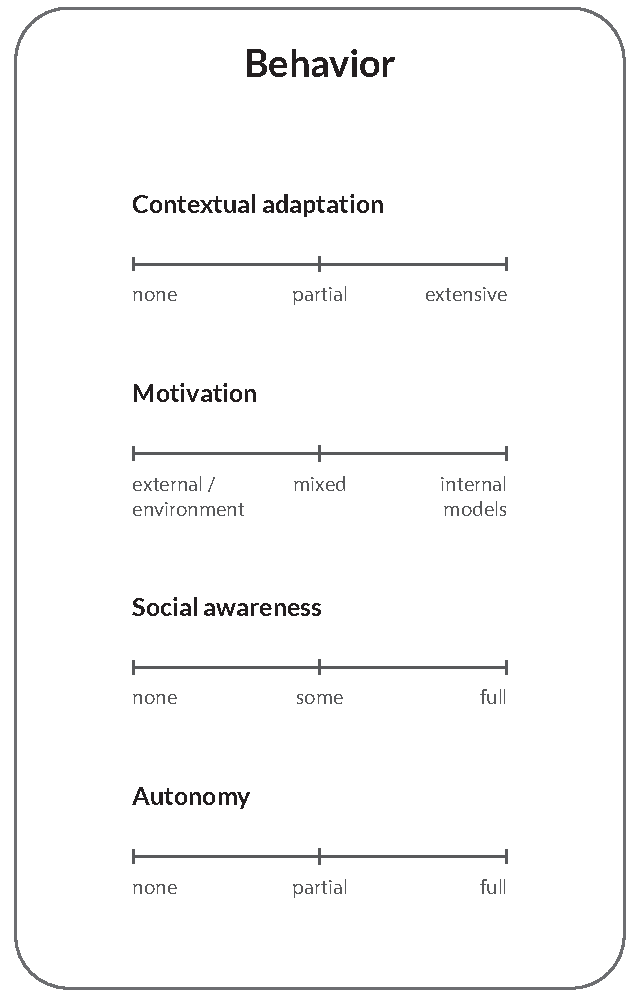
\includegraphics[scale=0.75]{images/solution_v4-05.pdf}
  \caption{Behavior design involves defining the level of contextual adaptation of the robots behavior, the motivation for behaviors, the level of social awareness evidenced in behavior, and the level of autonomous behaving of the robot.}
  \label{fig:behavior}
\end{figure}

The behavior dimension defines how the robot acts. Behavioral design is important, as the robot's behavior is one of the primary determinants of the user's attitude toward it, and contributes to its life-like impression \cite{designSpaces}. Behavior is defined by four qualities: contextual adaptation, motivation, social awareness and autonomy (as seen in figure \ref{fig:behavior}). ``Consistent, structured, simple behavior" guides the design of the behavior dimension. The design decisions made about the InMoov's behavior are seen in figure \ref{fig:behaviorFinal}.



\begin{figure}
\centering
  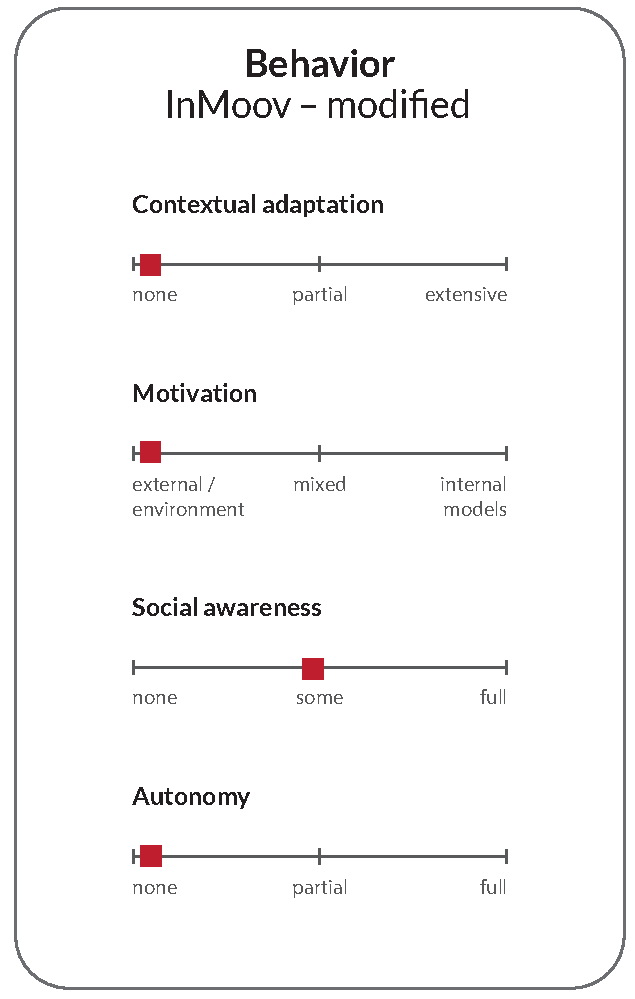
\includegraphics[scale=0.75]{images/solution_inmoov_final-05.pdf}
  \caption{The design decisions made about the InMoov's behavior in this solution are showed in red.}
  \label{fig:behaviorFinal}
\end{figure}


\subsubsection{Contextual adaptation}

Contextual adaptation of behavior refers to how much of the robot's behavior has been defined beforehand by its creator, and how much the robot can independently determine its behavior according to the context. The levels of contextual adaptation of a robot's behaviour range from none, to partial, to extensive. Extensive adaptation is a description of human-like behavior, where the agent could improvise and adapt to different contexts and domains. Currently, to my knowledge, no robots exist that could perform a similar level of adaptation to humans. Behavior that can be classified as extensive contextual adaptation would involve the robot taking input from past situations that it has learned from, as well as the current context, and determining the best course of action according to these. If a robot were to perform on a similar level as a human, it would need to be able to learn to improve its decision making process and behavior according to success of past tasks. Robots that exhibit no contextual adaptation always follow the same course of action in a given situation. Their behavior is ``hard-coded".

At the time of writing, robots generally exhibit no contextual adaptation, or partial contextual adaptation. An example of partial contextual adaptation could be a robot behaving in a particular way in a given situation, but with randomized adaptations. By performing randomized behavior, a robot can modify its future behavior based on the best outcomes, and become more efficient in partial adaptation. For example, "artist robots" can create artwork by randomizing certain artistic styles onto pre-determined images. The choice of artistic style is based on data from previous sales of paintings, which leads to the robot attempting to improve its performance with each iteration. Here, while the robot appears to be behaving in a creative and improvisational manner, it does not take into consideration the context of the image being created. It also could not apply its artistic skills in another context. This leads to the behavior being classified as having partial contextual adaptation.

The behavior of the InMoov has no contextual adaptation. The signs and speech of the robot need to be pre-programmed. Hard coded behavior is also more consistent and structured than adaptation, which leads to less confusion for the child. Children can learn to imitate the robot more easily, due to the repetitiveness of the robot's imitation prompts. This follows the design guideline of ``consistent, structured, simple behavior". 


\subsubsection{Motivation}

Motivation of behavior describes whether the robot behaves purely in response to external stimulus from its environment, purely according to internal models, or a mix of the two. An example of motivation via internal models is the motivation system of the robot Kismet, in which behaviors are influenced according to internal models of Kismet's drives and emotions \cite{breazeal2004}.

In this solution, everything the robot does in the therapy situation is motivated by what the child is doing, which means that motivation is entirely external. The robot has no programmed ``internal models". Keeping the robot's behavior externally motivated follows the design guideline of ``consistent, structured, simple behavior", since children with autism have trouble anticipating other's internally motivated behavior due to lack of Theory of Mind \cite{baron1985does, frith2003autism}.



\subsubsection{Social awareness}

Designing social behavior to the right degree is difficult, as a robot may be perceived to have intentional behavior, due to its life-like appearance and behavior \cite{bartneck2004design}. Social robots should adhere to generally accepted social norms, in order to create the impression of possessing some form of social intelligence \cite{bartneck2004design, designSpaces}. Social awareness of a robot can range from none, to some, to full, although to my knowledge no robots with full social awareness currently exist. Arguably, this quality can vary also among humans. Social awareness means how well the robot follows social conventions, such as greeting a new person when they enter a room, maintaining appropriate personal distance to a human, or understanding when it is its turn to speak.

In this solution, sophisticated social abilities are not needed, as autistic children themselves have limited social abilities, and would be confused by a robot operating on the social level of a human. However, the InMoov does adhere to simple social norms, in order to teach them to the children. The InMoov greets upon meeting, says farewell when the user leaves, and acknowledges the user's presence by asking for their name. The robot also keeps eye contact, by looking in the general direction of the child. This was done by seating the child in front of the robot. No programmatic tracking of the child's face was implemented. The robot is also programmed to start and finish every sign with the same position, with fingers and arms resting at both sides freely. This helps indicate to the user when the robot's turn to speak starts and ends \cite{uluer2015new}. Keeping the level of social norms simple follows the design guideline of ``consistent, structured, simple behavior".


\subsubsection{Autonomy}

Autonomy defines to what degree a robot displays behavior in a self-contained manner. Autonomy of the robot's behavior can range from none, to some, to full. A robot that has no autonomy is operated externally by a human, and a robot that has full autonomy is completely self-contained in its operation. A robot with partial autonomy may occasionally need human intervention to behave appropriately.

The InMoov has no autonomy and is completely externally operated. However, it appears autonomous to the child, as the child's actions are being observed by a human operator from another room, who programs the robot to respond appropriately to the child. The human operating the robot follows a simple if-then do-while outline for the therapy. This makes the behavior of the robot straightforward and understandable for both the child. This follows the design guideline ``consistent, structured, simple behavior".


%%%%%%%%%%
%%%%%%%%%%

\section{Summary of the design}

This chapter introduced a design framework for the purpose of designing social robots, and detailed the process of using the framework. To my knowledge, no other frameworks that describe the entire design process of social robots exist.

The framework is utilized to make design decisions about a robot which is used to teach assistive sign language to children with autism. The robot selected for this solution is the open source humanoid robot InMoov. 

First, the problem space was defined, which involved defining the user group, their goal, safety and ethical considerations, and the robot's task. Based on the problem space, five design guidelines were established. The guidelines were used to guide the design of the solution space, which involved making decisions about the robot's environment, form, interaction and behavior. The implementation of the solution designed in this chapter is introduced in the next chapter.


\chapter{Methods}
\label{chapter:methods}

This chapter describes the research methodology used to examine the success of the design described in the previous chapter. The research setting, process and data analysis methodology are presented. 

The design in chapter \ref{chapter:design} involves many choices which may have affected the performance of the robot as a sign language tutor. Resources were not available to validate all of those choices. The interaction scheme of the robot was chosen as a likely candidate to influence tutoring effectiveness, and so the following study was designed. This study also serves as an example of how the design framework can be used more broadly: fixing other design parameters, and varying one to measure its effect of success.

Three different interaction schemes of the robot, referred to here as design conditions, were compared. The study of the robot's and the child's interaction was framed as a comparative design study. The research question relevant for this chapter is RQ2: Is the designed robot successful as an assistive sign tutor? This was examined by testing three hypotheses: 


\vspace{3mm}

\noindent\textbf{H1: Children will imitate signs performed by the robot}
\vspace{3mm}

\noindent\textbf{H2: The design condition will affect the success of imitation}
\vspace{3mm}

\noindent\textbf{H3: The design condition will affect the child's attention focus}
\vspace{3mm}

These hypotheses, and how they were tested, is discussed further in this chapter.


\section{Research setting and process}

Experiments with 12 autistic children were organized to examine their responses to the robot InMoov as an assistive sign tutor. The experiments were organized at Satakunta's hospital district, in collaboration with speech therapist Lehtonen and neuropsychologist Nyman. A script for the robot to follow during the experiments was created together with the speech therapist. The experiments lasted around 30 minutes per child, with the speech therapist and a companion of the child (parent or other care-taker) present with the child in the experimentation room. The robot was operated from the next room by myself and another engineer, according to instructions given by the speech therapist via a camera feed. The therapy session was observed by the operators through three camera feeds. After the therapy session, the child and their companion were asked to fill out short surveys to describe their experience. The surveys along with footage from the camera feeds were analyzed after the experiments, using both quantitative and qualitative methods.


\subsection{The InMoov and its modifications}

The InMoov is a human-sized humanoid robot torso, controlled by Arduino microcontrollers, constructed out of 3D printed plastic body components and gears. The power is distributed through custom printed circuit boards, also available under the CC BY-NC license. The fully assembled robot has 29 servo motors controlled by two Mega Arduino boards. A USB hub connects the Arduino boards and peripherals (in our case a mouth speaker and an eye camera) to the controlling computer, which in this case was a Windows laptop. The software used to control the robot, MyRobotLab, is an open source robot control framework \cite{inmoov}. 

\begin{figure}
\centering
  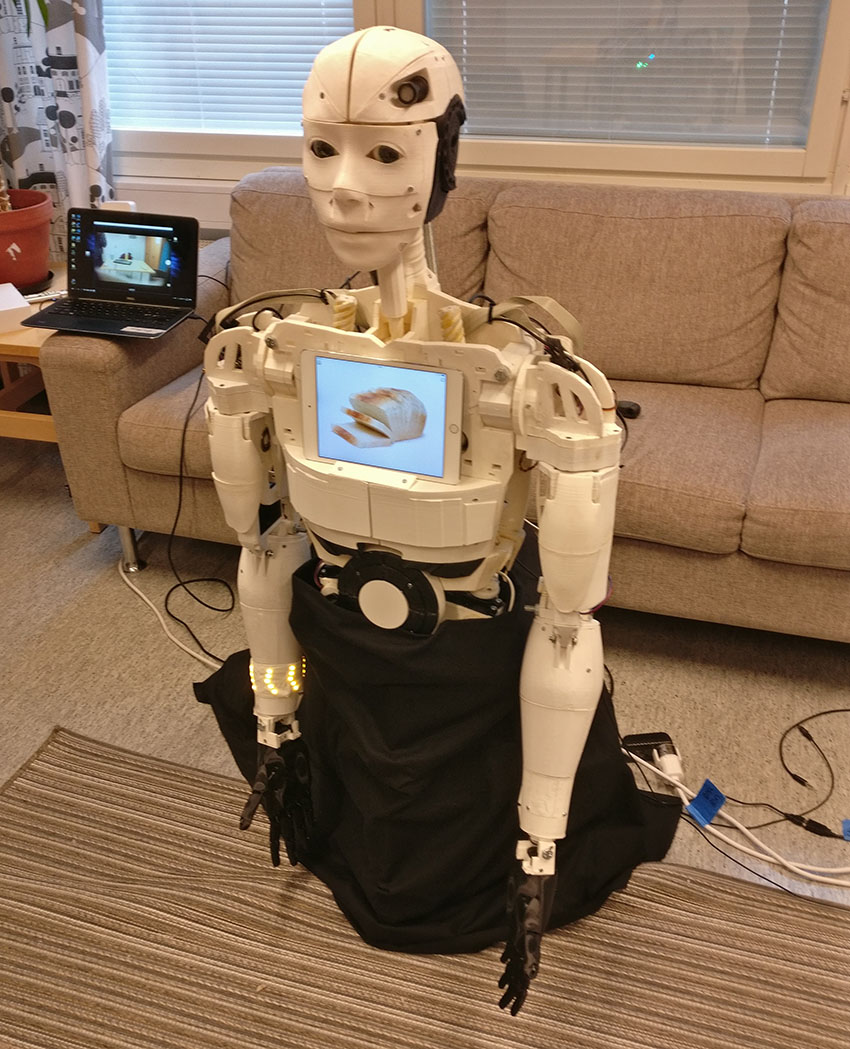
\includegraphics[width=8cm]{images/momo_on_floor.jpg}
  \caption{The robot pictured in the experimentation room, with both the lights on the hand and the picture on the tablet active.}
  \label{fig:momo}
\end{figure}

The implementation of the InMoov used in this experiment can be seen in figure \ref{fig:momo}. The InMoov used in this experiment was built using the original schematics, and printed out of ABS and PLA plastic, with additional NinjaFlex in the hands. Its original hands were replaced by Ada hands, the schematics for which are also available online under a Creative Commons license CC-BY-SA \cite{adaOpenbionics}. The original hands are visible in figure \ref{fig:inmoovhands}, while the new hands are visible in figure \ref{fig:adahands}. The signs were performed solely with the robot's arms and hands. The InMoov had 2 degrees of freedom (DOF) in each finger, including its thumb. Its wrists had 2 DOF, biceps 4 DOF, and shoulders 4 DOF. The InMoov was powered by an adjustable bench power supply with 6 V. The Ada hands were powered through two 12 V AC adapters.

\begin{figure}
\centering
  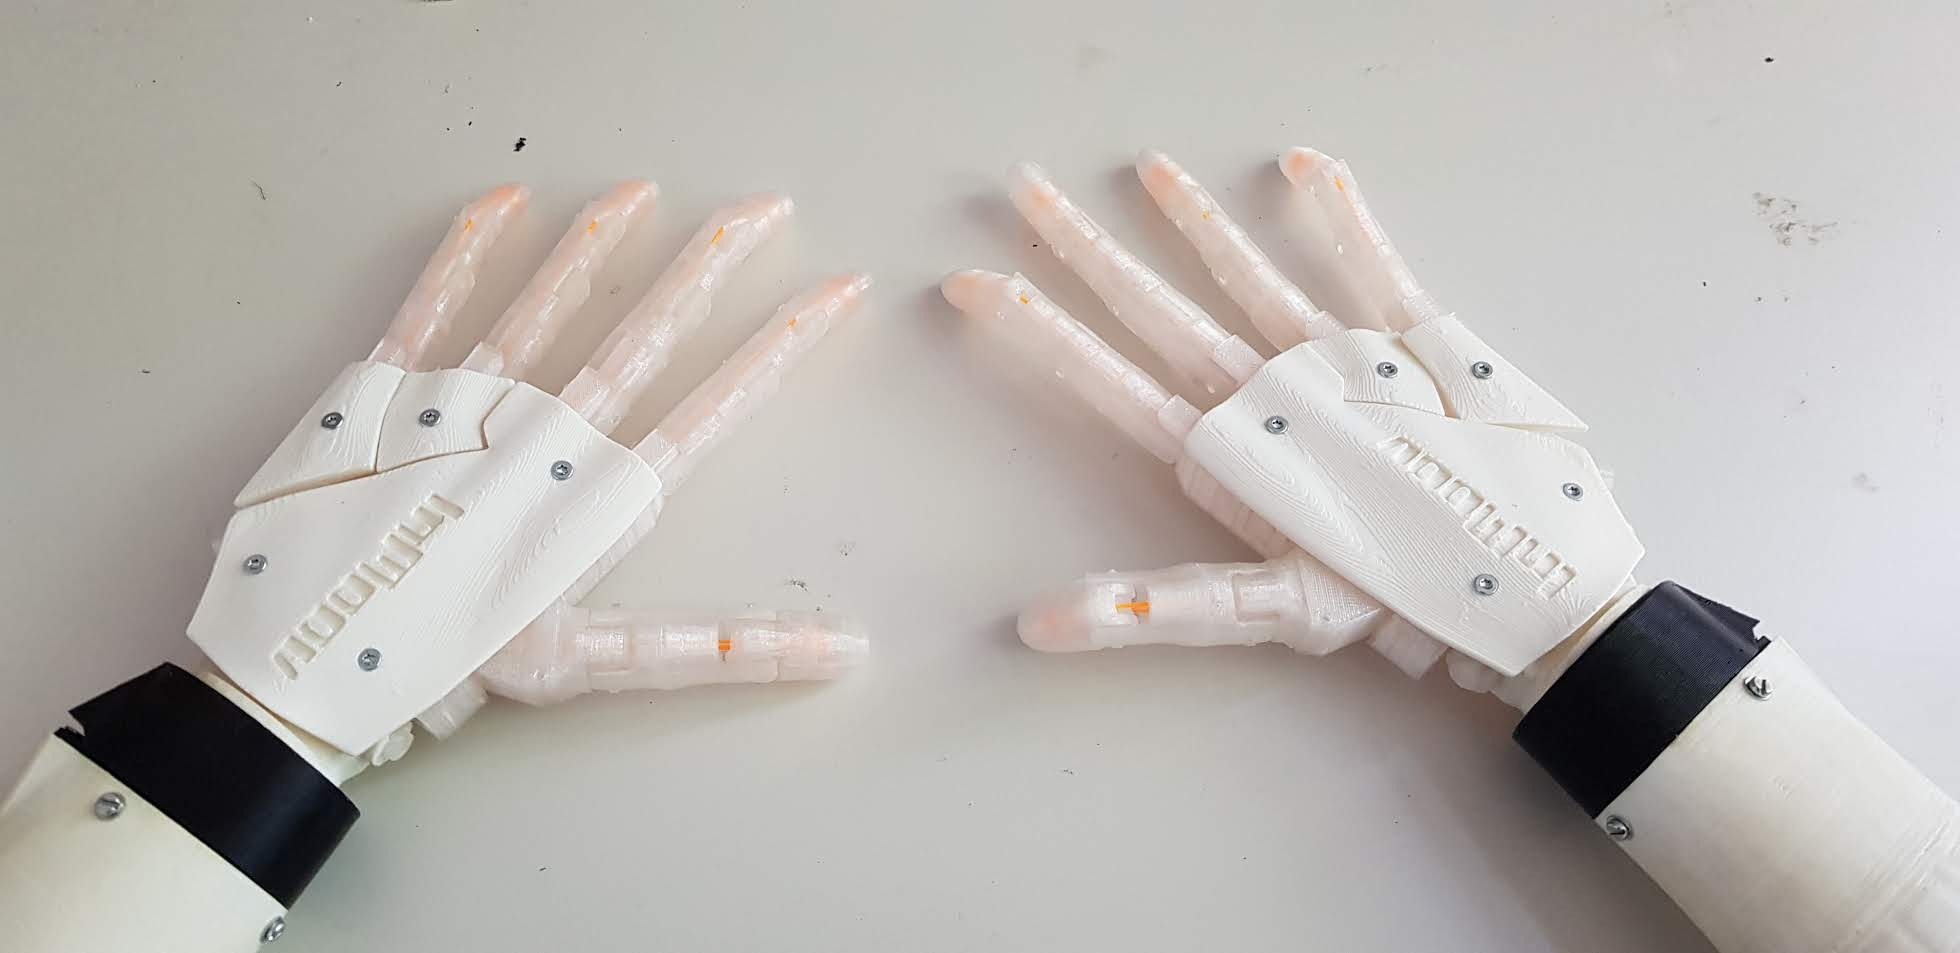
\includegraphics[width=\linewidth]{images/Inmoov-hands.jpg}
  \caption{The InMoov's original hands.}
  \label{fig:inmoovhands}
\end{figure}

\begin{figure}
\centering
  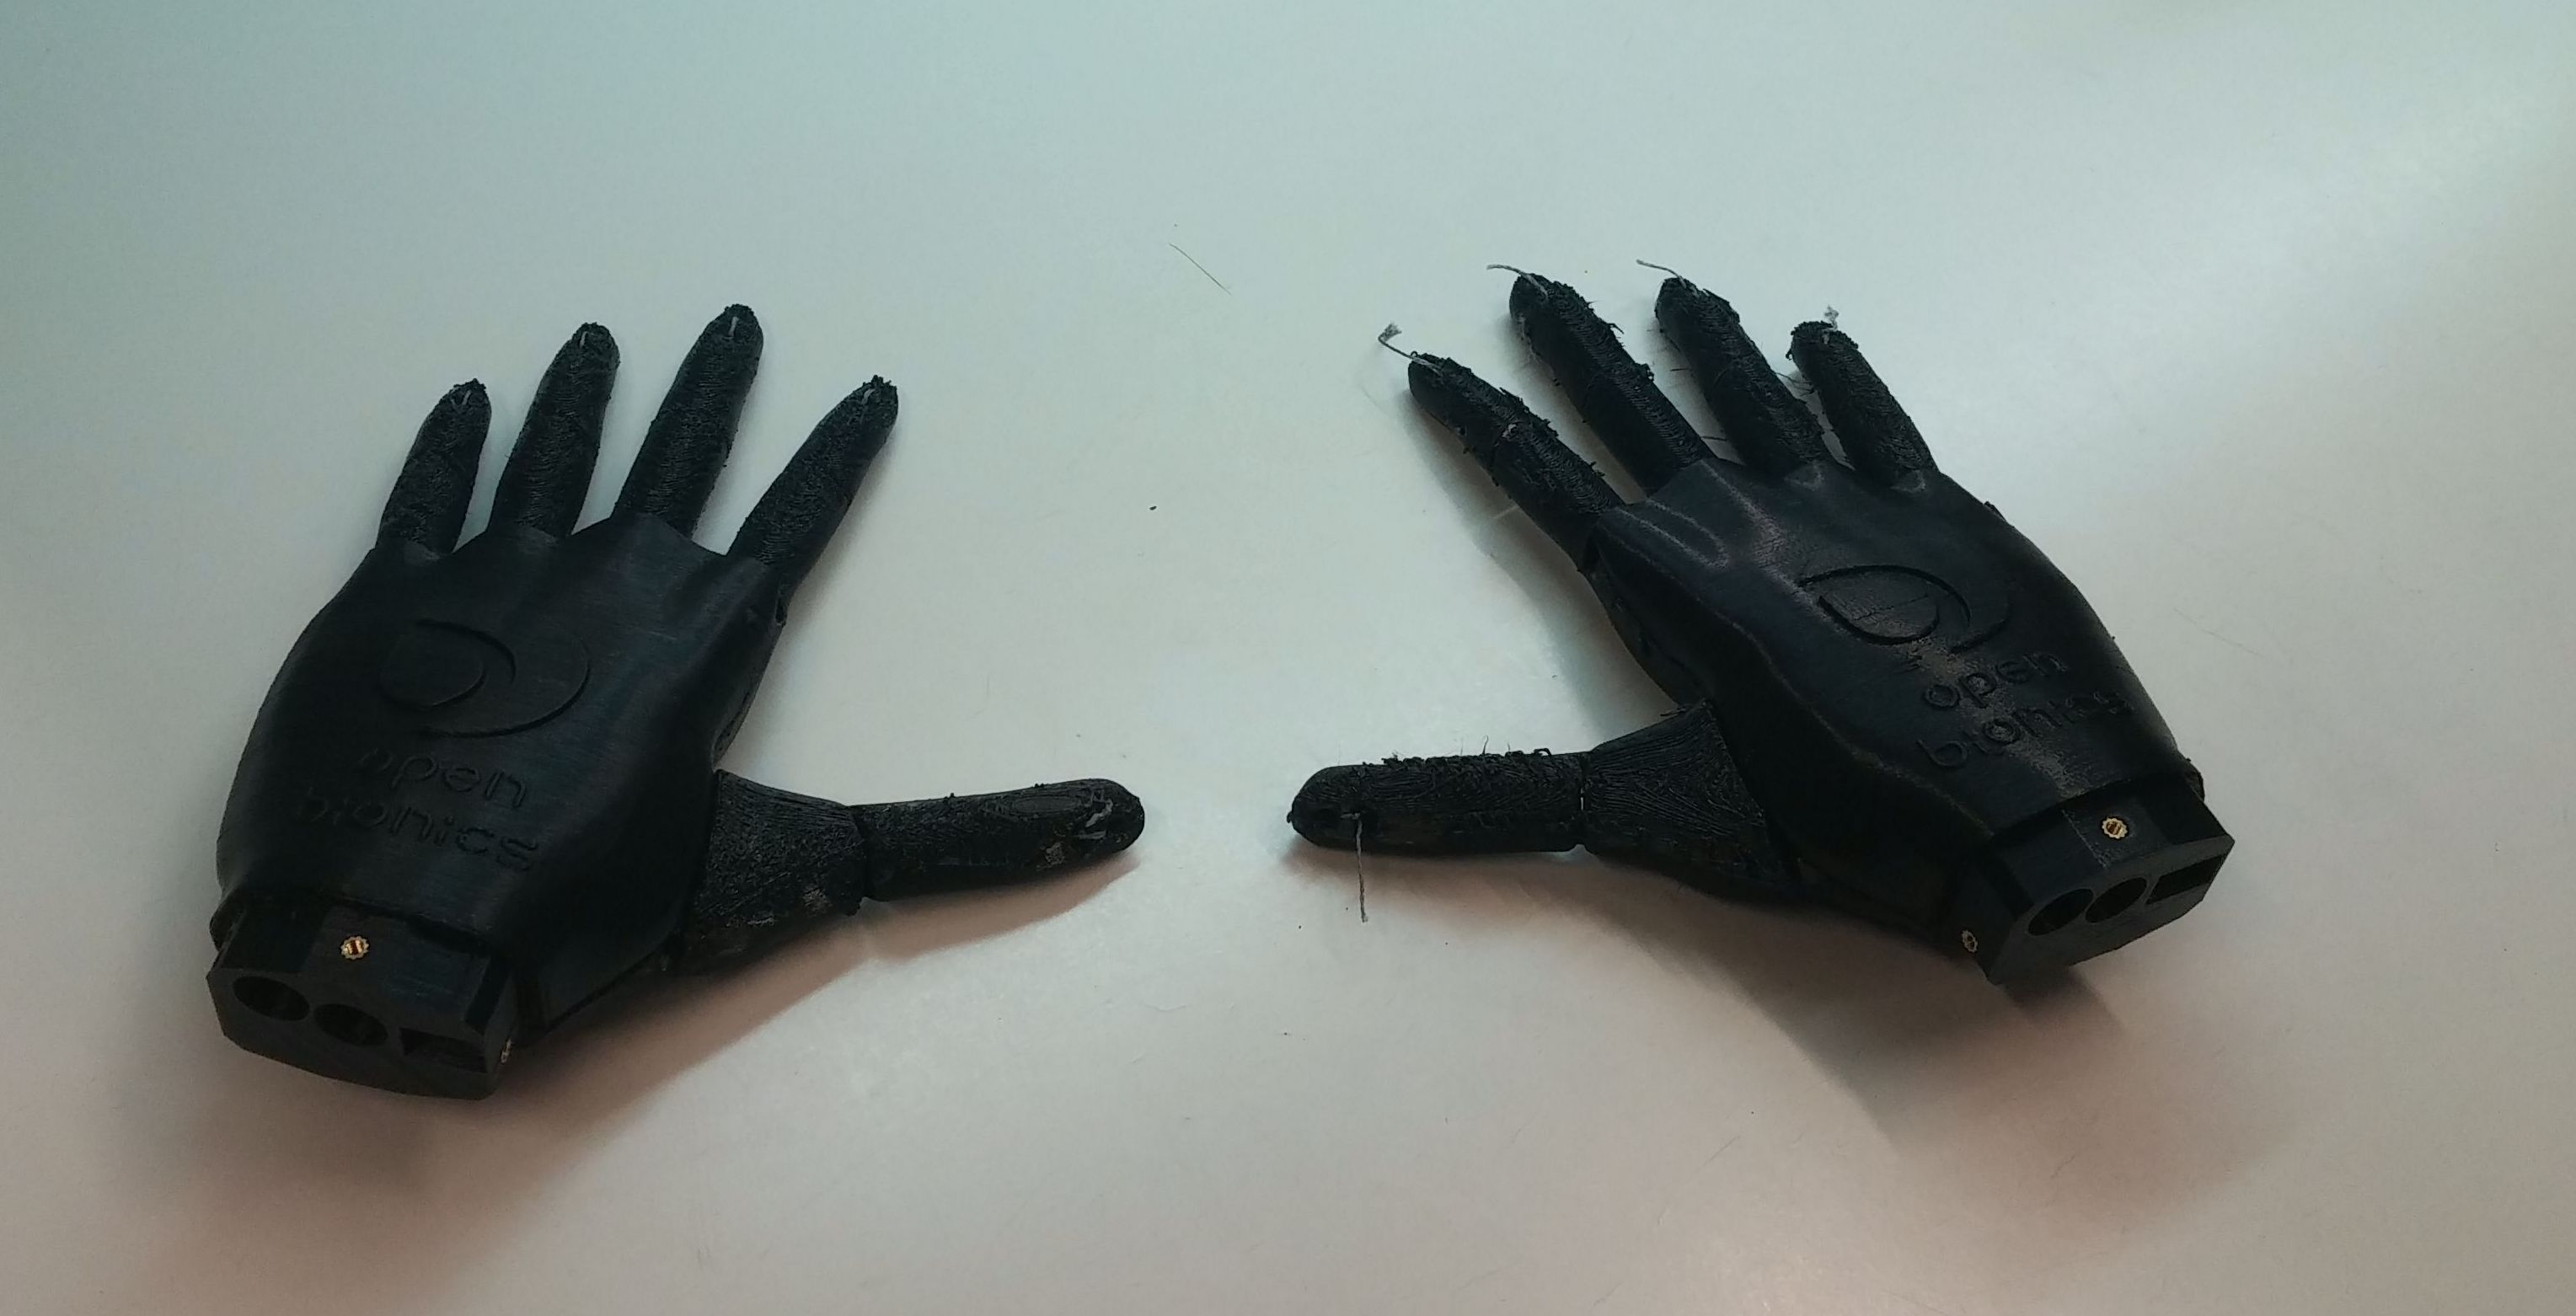
\includegraphics[width=\linewidth]{images/Ada-hands.jpeg}
  \caption{The new Ada hands.}
  \label{fig:adahands}
\end{figure}

The InMoov's chest components were modified to fit a tablet screen, and lights were attached to its right hand with tape. To control the robot during the experiments, commands were executed through MyRobotLab. Unique command sequences were written for each child, which were executed according to what the operators observed to be happening in the experiment room. The tablet in the robot's chest was also controlled through MyRobotLab.


\subsection{Signing with the InMoov}

9 signs were selected for the experiment together with the speech therapist. The signs are depicted in figures \ref{fig:viittomat1} and \ref{fig:viittomat2}. The thumbs up gesture that the robot performs during the experiments is also depicted in figure \ref{fig:viittomat2}. When choosing these signs, the physical limitations of the InMoov were taken into account: the InMoov is unable to cross its arms over its midsection, could not raise its shoulders, and could not bend its wrists. All of the signs were non-abstract concepts, such as animals or sports, which children were familiar with beforehand. These signs would be taught in assistive signing therapy even without the robot. Before the signs were used in the experiments, the speech therapist verified the recognizability of the signs with a colleague who did not know the set of signs. This procedure was adapted from the sign language study performed with Robovie R3 \cite{uluer2015new}.


\begin{figure}
\centering
  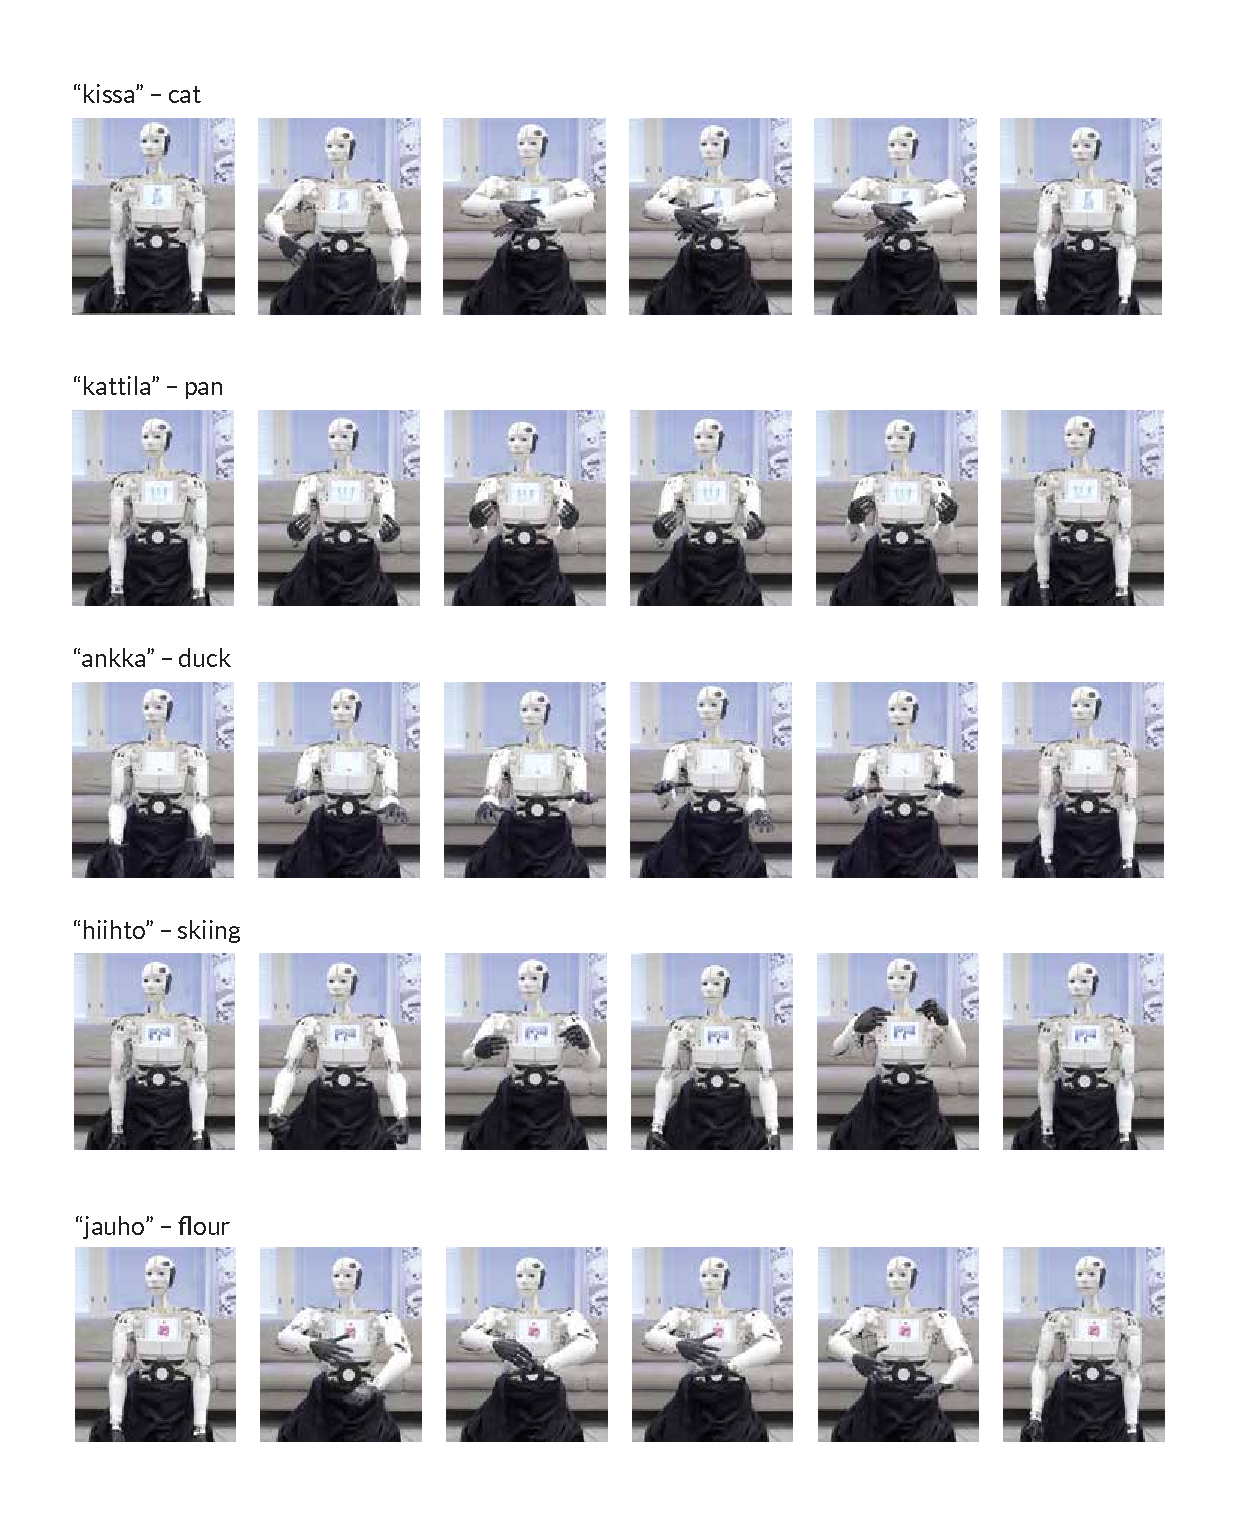
\includegraphics[width=\linewidth]{images/viittomat1.pdf}
  \caption{Five signs out of the set of nine.}
  \label{fig:viittomat1}
\end{figure}

\begin{figure}
\centering
  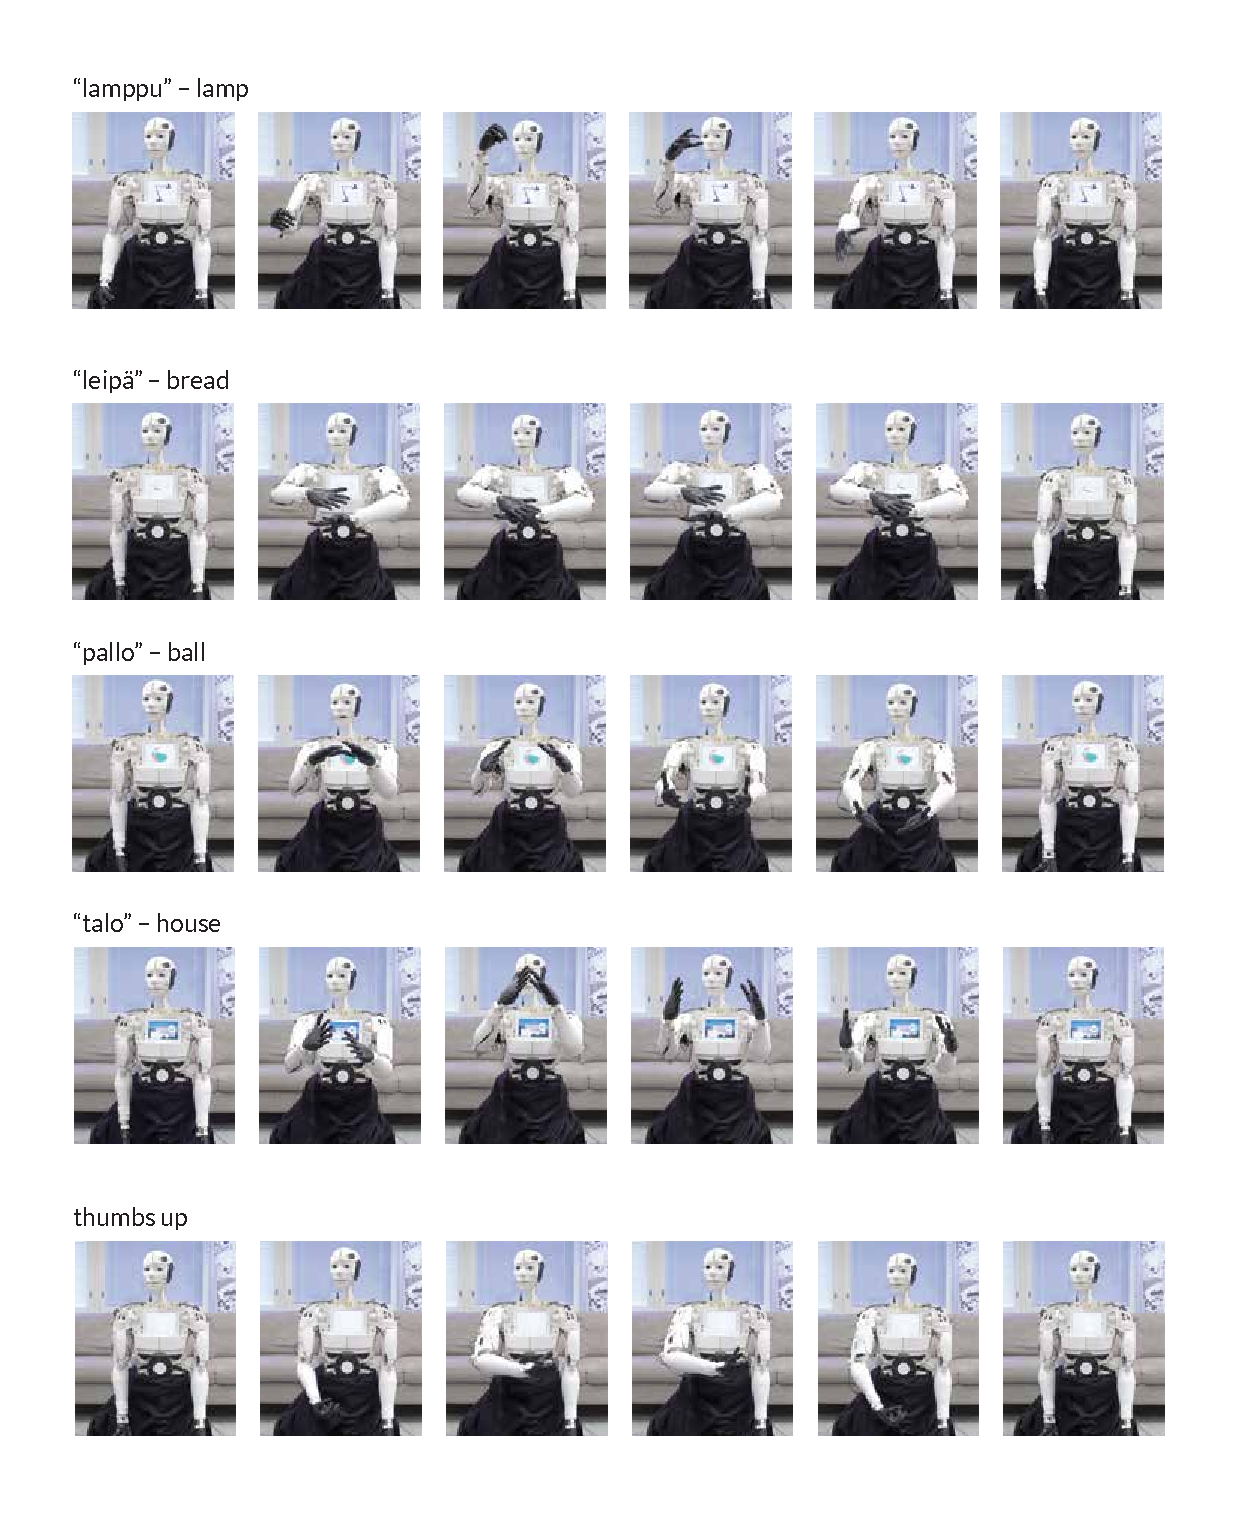
\includegraphics[width=\linewidth]{images/viittomat2.pdf}
  \caption{Four signs out of the set of nine, and the thumbs up gesture that the robot makes to reward the child.}
  \label{fig:viittomat2}
\end{figure}


\subsection{Research participants}

10 out of the 12 children that took part in the experiments were analyzed. Two of the experiments had to be discarded from data analysis, one due to a mistake in the operation of the robot, and the other after the child's parent stopped the experiment since the child could not calm down. The participants' ages, severity of autism and companions in the experiment are detailed in table \ref{table:participants}.


\vspace{0.5cm}
\bgroup
\def\arraystretch{1.3}
\begin{table}
\centering
\begin{tabular}{ c | c | r }
  \textbf{Age} & \textbf{Autism severity} & \textbf{Accompanying person(s)}\\
  \hline
  13 & mild & mother \\
  23 & severe & caretaker \\
  14 & severe & caretaker \\
  13 & severe & mother \\
  14 & mild & mother \\
  11 & severe & mother \\
  16 & severe & caretaker and psychologist \\
  14 & severe & two caretakers \\
  11 & mild & mother and father \\
  16 & severe & two caretakers \\
\end{tabular}
\vspace{0.5cm}
\caption{A list of the experiment participants' ages, autism severity, and accompanying persons.}
\label{table:participants}
\end{table}
\egroup


\subsection{Experiment set-up}

The experiment was set up in a room at the facilities of Satakunta's hospital district, in collaboration with speech therapist Lehtonen and neuropsychologist Nyman. The experiment set-up is seen in figure \ref{fig:roomSetup}. The experimentation room was familiar to some of the children beforehand. Some of the children came from home, and some lived at the hospital's quarters. All children were accompanied by either a parent or a caretaker from the hospital.

\begin{figure}
  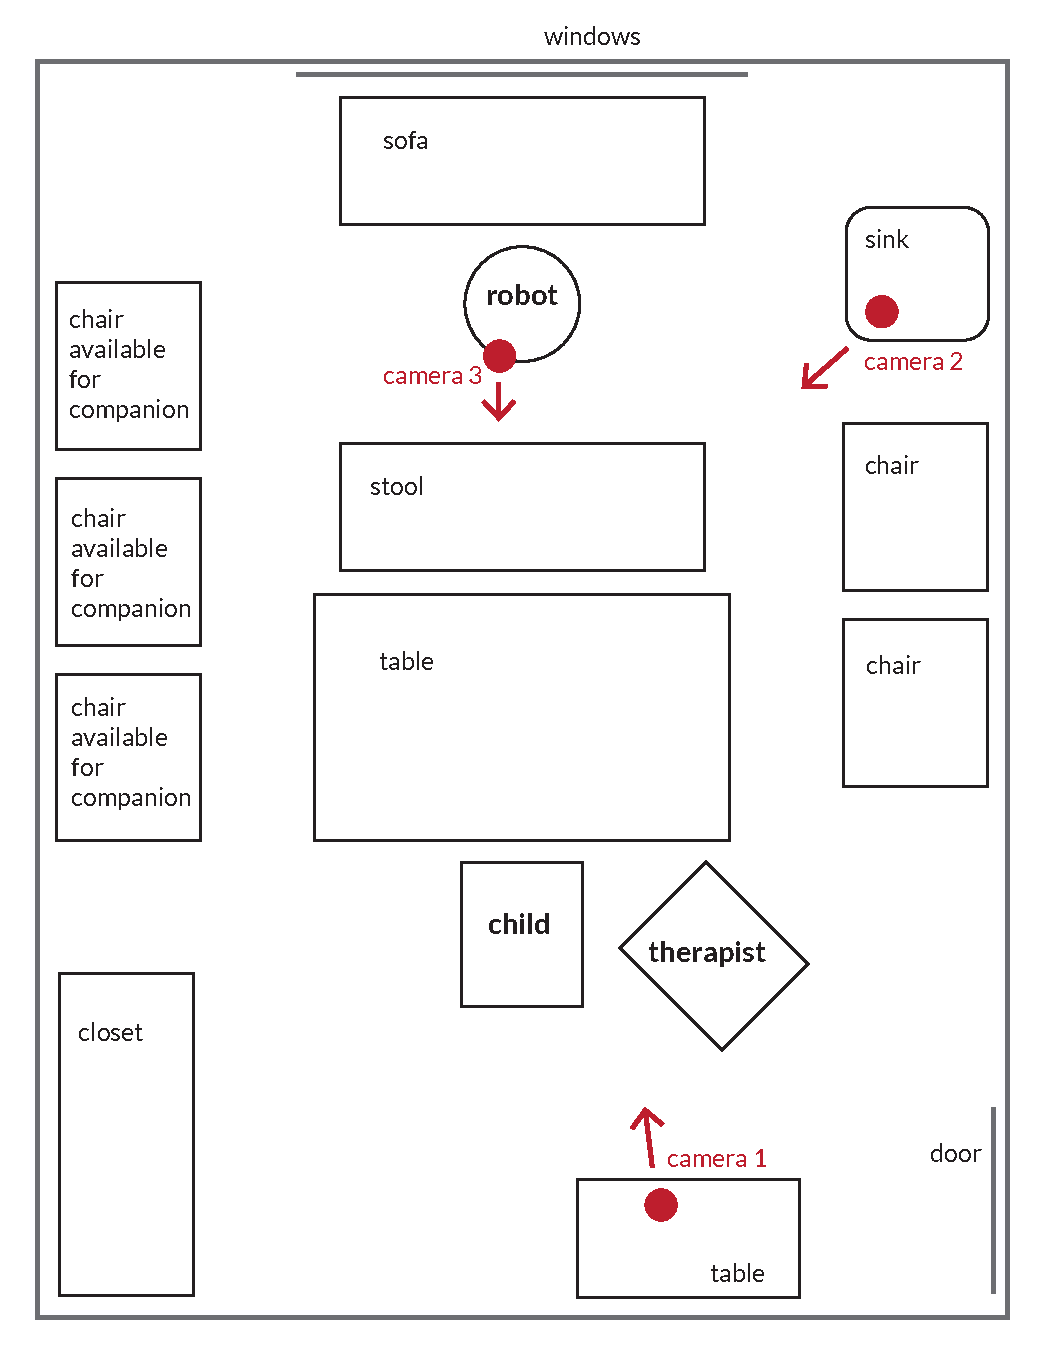
\includegraphics[width=\linewidth]{images/room_setup.pdf}
  \caption{The experiment set-up. The child sat directly in front of the robot, with a table in between them, for the safety of the child. The speech therapist sat next to the child, facing the child and the robot. Three cameras were placed in the room, in order to capture all of the child's behavior. The child's companion could choose one of the three seats on the side of the room.}
  \label{fig:roomSetup}
\end{figure}

The robot was at the back of the room on the floor. The child was sat at a table directly facing the robot. The speech therapist sat diagonally next to the child. The companion of the child sat in one of the chairs along the sides of the room, wherever they felt most comfortable.

The table was placed between the user and the robot to discourage physical contact in order to ensure physical safety of the child, and of the robot, as the robot is fragile. Some of the test users were also known to display aggressive behavior on occasion, so the table acted as a protector of both the robot and the child.

The robot was teleoperated from a room across the hall. An observer observed the experiment room through three camera feeds, and told the operator which functions to execute, according to the speech therapist's signals. The speech therapist indicated to the operator that the child signed correctly, incorrectly, or that the child had not responded as all. Cameras were placed behind the child, to the front of the child, and in the robot's right eye. The view front the front camera can be seen in figure \ref{fig:front}, and the back camera in figure \ref{fig:back}. In accordance to the ethics consideration defined in the design process, the footage recorded by the cameras that was used to generate data was treated with care, and kept encrypted.

\begin{figure}
\centering
  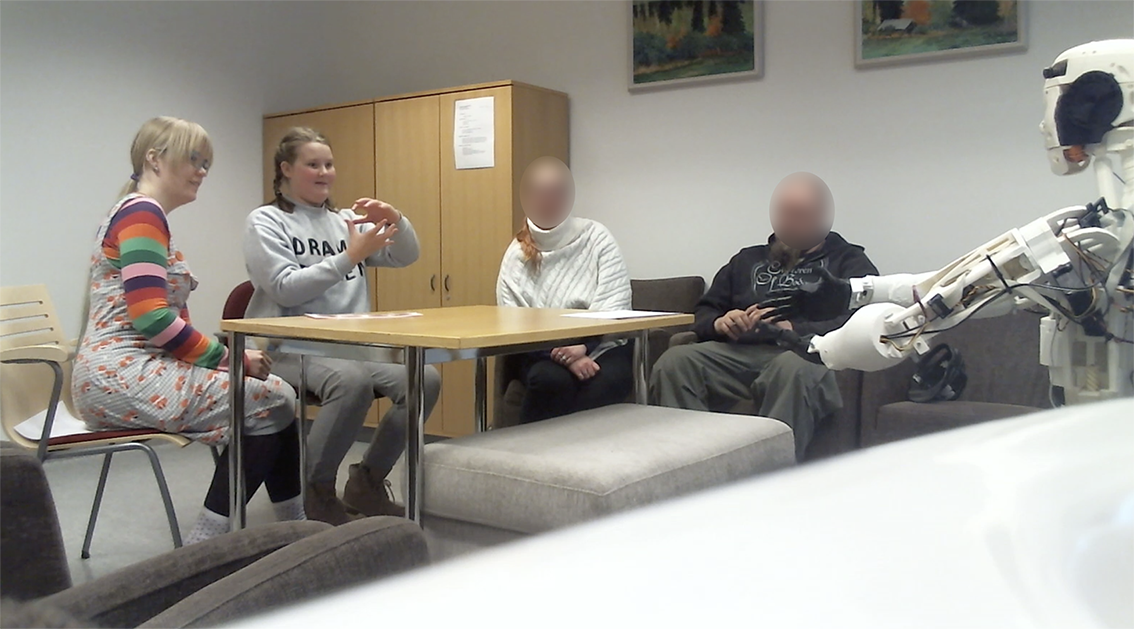
\includegraphics[width=\linewidth]{images/experiment_front.png}
  \caption{View from the front camera, with the robot signing ``flour".}
  \label{fig:front}
\end{figure}

\begin{figure}
\centering
  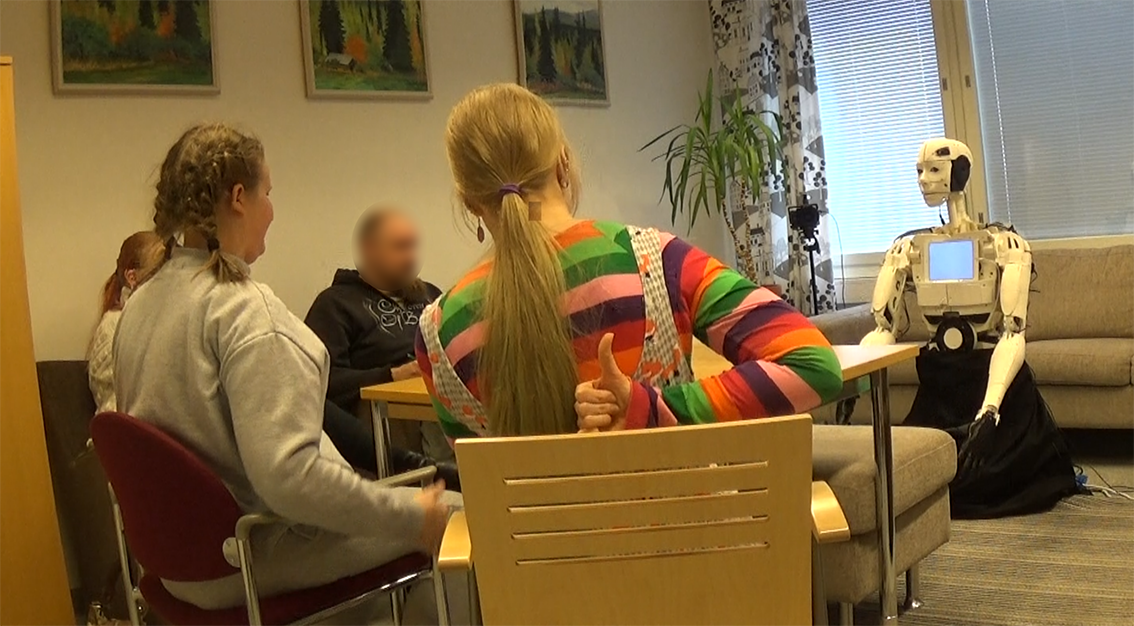
\includegraphics[width=\linewidth]{images/experiment_back.png}
  \caption{View from the back camera, with the speech therapist showing to the camera that the child had signed accurately.}
  \label{fig:back}
\end{figure}


\subsection{Experimental procedure}

The experimental procedure was precisely defined beforehand, as was discussed in the previous chapter.

When the child first entered the experimentation room, the speech therapist showed the child a picture series of how the experiment would proceed. This procedure was adapted from the study done with the robot Tito and children with autism \cite{duquette2008exploring}. The picture series is visible in appendix \ref{chapter:explanation}. This was done to create some familiarity with the robot so the child could feel more comfortable \cite{duquette2008exploring}, and to help the child know what to expect. After the experiment ended, the child and their companion were asked to give their opinions via surveys. The child's survey is visible in appendix \ref{chapter:children}, and the companion's survey is visible in appendix \ref{chapter:companions}. The survey was administered by neuropsychologist Nyman, who entered the experiment room after the interaction with the robot had concluded. After completion of the surveys, the child and their companion promptly left the experimentation room.

For the experiments themselves, an interaction structure was programmed beforehand for each child. The programmed interaction structure included each child's name, and a randomized order for the signs. For each sign, one of three different design conditions was randomized. Three signs were assigned randomly to each condition. The design conditions were made up of different interaction modalities. The design conditions were:

\begin{itemize}
  \item Sign and voice command
  \item Sign and voice command, and image in chest tablet
  \item Sign and voice command, and flashing lights in right hand
\end{itemize}

The image condition can be seen in figure \ref{fig:momo}, and the images shown on the tablet are seen in figure \ref{fig:tabletimages}. The image always corresponded with the word being signed. The lights on the robot's hand can be seen in figures \ref{fig:lights} and \ref{fig:momo}. The lights were turned on when the robot started signing, and switched off when it stopped signing.

\begin{figure}
\centering
  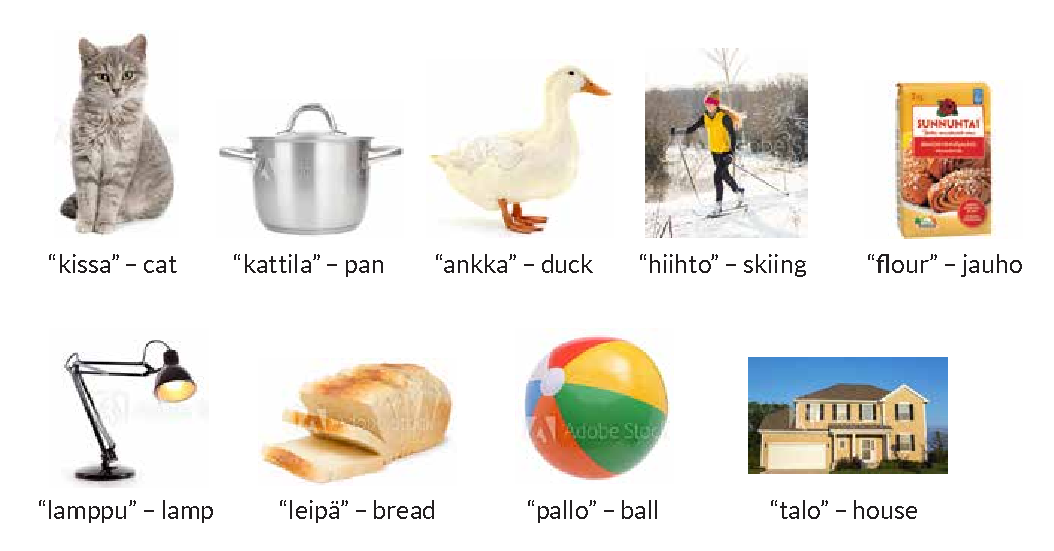
\includegraphics[width=\linewidth]{images/tablet_images.pdf}
  \caption{Images shown on the tablet simultaneously with the word spoken in the second design condition.}
  \label{fig:tabletimages}
\end{figure}

\begin{figure}
\centering
  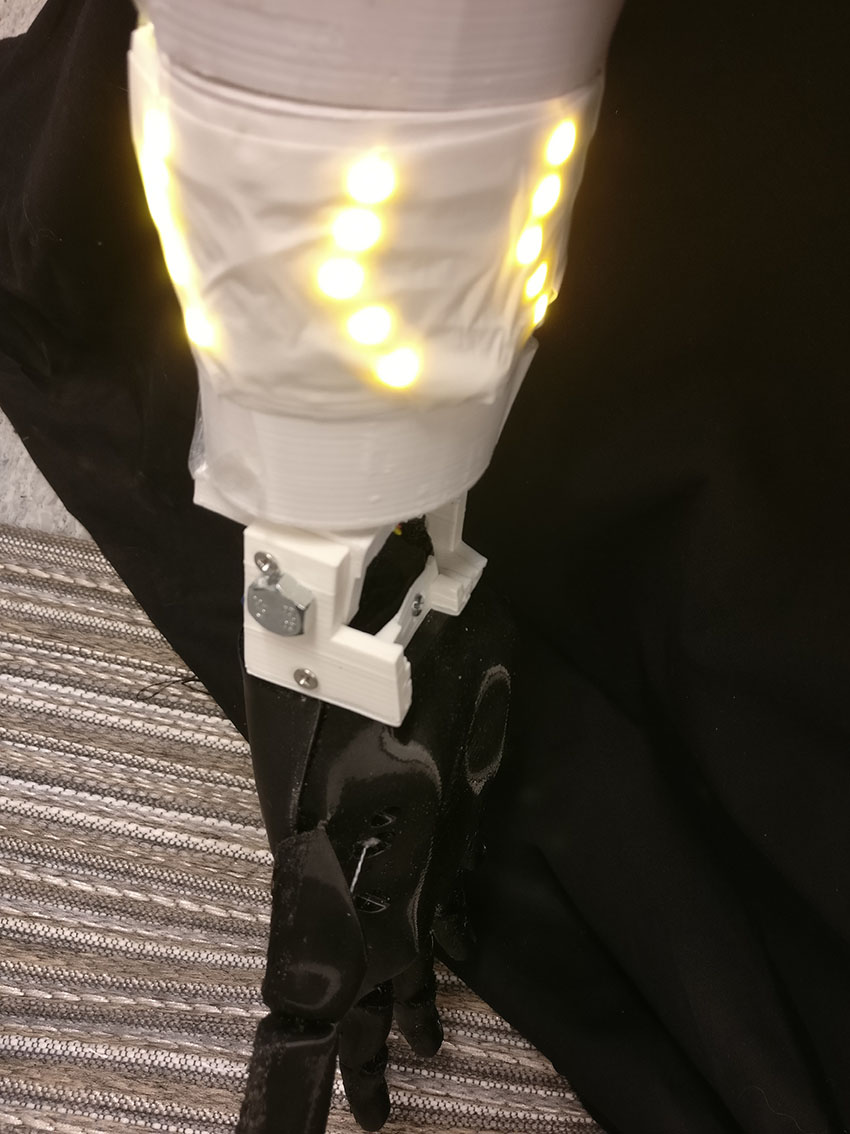
\includegraphics[width=4cm]{images/lights.jpg}
  \caption{The lights attached to the robot's hand for the third design condition.}
  \label{fig:lights}
\end{figure}

The basic interaction structure used during the experiments is depicted in figure \ref{fig:flowchart}. The robot demonstrated a sign, asked the child to respond, and then responded appropriately to the child's response. The robot demonstrated nine signs overall during each experiment. At the start of the experiment the robot said hello, and at the end of the experiment the robot said goodbye. A more detailed conversation transcript is attached in appendix \ref{chapter:conversation} in Finnish.

\begin{figure}
\centering
  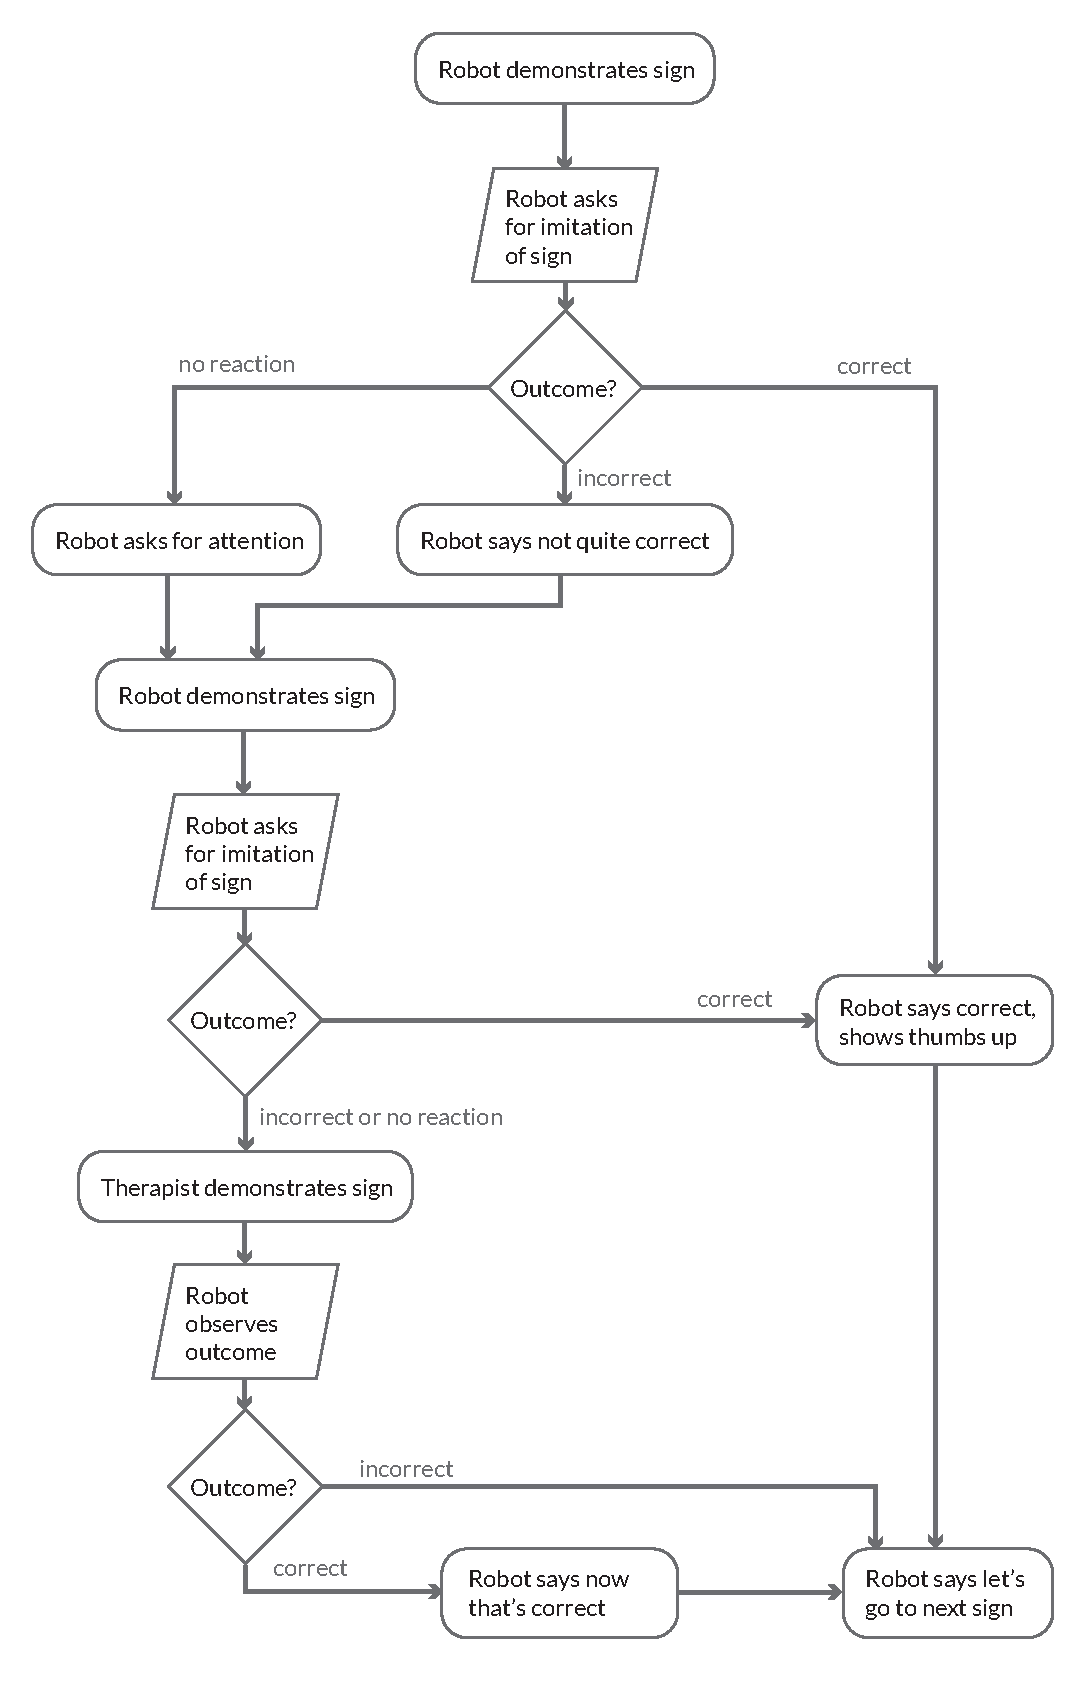
\includegraphics[width=\linewidth]{images/behavior_flowchart.pdf}
  \caption{Flowchart of the robot's behavior, which was executed by the operators according to the child's responses.}
  \label{fig:flowchart}
\end{figure}

%%%%%%%%%%
%%%%%%%%%%


\section{Research methodology}

The primary research methodology was examining and analyzing the videos of each child interacting with the robot. Due to the small amount of quantitative data anticipated to be gathered from the videos, it was triangulated with qualitative data gathered from the surveys conducted with the children and their companion after the experiment.

H1, H2 and H3 were tested primarily through the video data, and resulting conclusions were supported by qualitative data from the surveys.


\subsection{Quantitative measures}

Two quantitative measures were selected to be analyzed from the videos to evaluate the success of the robot as an assistive sign teacher. Firstly, the success of the child's imitation was analyzed. Secondly, the child's attention on the robot and other objects was analyzed.


\subsubsection{Imitation}

Imitation has been used as a measure of success in previous studies examining the use of robots in autism therapy with children \cite{robins2004effects, robins2006appearance, goodrich2012incorporating, duquette2008exploring, boccanfuso2017low}, as well as teaching sign language to neurotypical children \cite{taleofarobot, uluer2015new}.

Imitation has two functions: communication and learning. These two functions imply capacities such as detection of novelty, attraction toward moving stimuli and perception-action coupling. It is argued that basic perception-action coupling is intact in autistic children \cite{nadel2004toward}.

Imitation can be described as having several levels: at a low level of functioning, children with autism may produce perception-action coupling and imitate movements that they see, without an explicit intention to do so. At a higher level, imitative behavior is informed by the intention to do as the other intends to do. An even higher level is communicative imitation, where the imitator has the intention to do as the others intend for them to do \cite{meltzoff2002imitative}. In this experiment, types of imitation are not distinguished from each other, and even rudimentary perception-action coupling is accepted. However, for further experiments, different types of imitation should be considered.

Children's responses to the robot's signs were categorized into four categories: correctly imitating the robot, correctly imitating the robot with human assistance, incorrect imitation of the robot, and no reaction to the robot's imitation suggestion.

Correct imitation with human assistance was measured as a separate category, as there could be no certainty whether the child had in fact imitated the robot or the human. If the child imitated the human, it could not be taken as an indicator of the success of the robot as a teacher. Human assistance was defined as either the therapist or the companion signing simultaneously or after the robot, after which the child signed correctly.

The robot asked for each sign up to two times. The response given on the latter request was recorded: if the child signed incorrectly or did not respond on the first request, but signed correctly on the second request, the response was recorded as correct.

H1 was tested by determining overall imitation success. Imitation success was compared across the three design conditions. This directly tested H2. 


\subsubsection{Gaze direction}

The other quantitative measure selected was eye gaze direction, which has also been used in previous studies examining the success of using a robot in autism therapy \cite{ARIA, duquette2008exploring, goodrich2012incorporating, kozima2009keepon, pop2013social, robins2004effects, wainer2014pilot}. The specific attention analysis methodology used was adapted from a previous study observing interactions of children with autism \cite{joseph1997investigation}. Gaze direction was categorized into four categories: robot, therapist, loved one, and elsewhere or unfocused. When the gaze direction was obscured, the time of obscuration was discarded from the analysis.

Gaze directed at an interaction partner is a sign of initiation of contact, and its maintenance. Gaze is the indicator of social accessibility \cite{goffman2017interaction}. Individuals with ASD may be slower to be direct their gaze at their interaction partner, and the timing of gaze may differ from neurotypical people \cite{kendon1967some}. In this case, gaze directed at the robot is used as a measure of success of contact between the child and the robot.

Gaze directed at the robot was measured as a percentage of the time spent in interaction, as times varied between interaction instances, and between children. Gaze was measured from the videos by observing the child's gaze focus from each frame. Gaze directed at the robot was defined as the child looking at the robot's face, torso or hands.

The gaze direction was compared across the three design conditions. This directly tested H3.


\subsection{Qualitative methods}

Qualitative methods used were surveys conducted with the children and their companions, where they were asked for their opinions about the robot.

Children were asked how they felt about the robot and its design conditions right after the experiment. Their companion was asked how they thought the child felt about the robot, and how they would rank the usefulness of the design conditions. Companions were also asked whether they thought the child formed a connection with the robot, and if they could benefit from using it as a tool. The companions were also asked how they felt about the robot. Some of the questions were quantifiable, while others provided the opportunity to give a free-form answer.

The simpler answers were quantified, while the free-form text was analyzed for recurring themes. Out of 10 children, 6 were able to answer the questions reliably. Out of 10 companions, 8 turned in the survey, with most questions answered.

The symptoms of autism vary greatly from person to person. Because of this, qualitative data gathered from these interviewees is not directly generalizable to the entire autistic population. However, this is always the case with user interviews: one person's perspective does not necessarily represent the whole. The qualitative data gathered was used to create a general sense of direction for future designs of the robot, or other robots used for the same purpose. The qualitative data was used to support the answers provided by the quantitative methods for hypotheses H1, H2 and H3.

 
\chapter{Results}
\label{chapter:results}

The aim of the study was to examine the effect of three design conditions on outcomes. The design conditions were three different interaction schemes: the robot signs and says the word in question (abbreviated in tables as ``Sign only"); the robot signs, says the word in question and shows an image of the word (abbreviated in tables as ``Image"); and the robot signs, says the word in question and flashes lights (abbreviated in tables as ``Light").

First, quantitative analysis of the child's responses to the robot's signs and the child's gaze direction are presented. Second, the qualitative analysis of the surveys conducted with the children and their companions is presented.

As a reminder, the hypotheses tested in the experiments were:
\vspace{3mm}

\noindent\textbf{H1: Children will imitate signs performed by the robot}
\vspace{3mm}

\noindent\textbf{H2: The design condition will affect the success of imitation}
\vspace{3mm}

\noindent\textbf{H3: The design condition will affect the child's attention focus}
\vspace{3mm}


%%%%%%%%%%
%%%%%%%%%%


\section{Quantitative analysis}

The Wilcoxon signed-rank test is used to examine the success rate of the children's imitations of the signs. The Wilcoxon test is a non-parametric statistical hypothesis test, and is used to perform a one-sample test to determine whether the median number of imitations is statistically significantly different from zero \cite{wilcoxon1945individual}. The Friedman test was used to analyze the potential effect of the three different design conditions on both the child's ability to sign accurately and the child's gaze direction. The Friedman test is a non-parametric test, and is used to detect differences in outcomes across multiple test attempts \cite{friedman1937use}. An $\alpha$ level of $0.05$ was used for all statistical tests.


\subsection{Successful imitation of signs}

\begin{table}
  \centering
  \renewcommand{\arraystretch}{1.2}
  \begin{tabular}{|p{3cm}|c|c|c|c|}
    \hline
    \textbf{Child} &
    \textbf{Sign only} &
    \textbf{Image} &
    \textbf{Light} & 
    \textbf{All}\\
    \hline
    A & 2 & 2 & 1 & \textbf{5}\\ \hline
    B & 2 & 3 & 1 & \textbf{6}\\ \hline
    C & 2 & 3 & 2 & \textbf{7} \\ \hline
    D & 0 & 0 & 0 & \textbf{0} \\ \hline
    E & 3 & 3 & 3 & \textbf{9} \\ \hline
    F & 0 & 0 & 0 & \textbf{0} \\ \hline
    G & 0 & 0 & 0 & \textbf{0} \\ \hline
    H & 0 & 1 & 3 & \textbf{4} \\ \hline
    I & 3 & 3 & 3 & \textbf{9} \\ \hline
    J & 2 & 2 & 1 & \textbf{5} \\ \hline

  \end{tabular}
 
  \caption{Successful imitations of each child in different design conditions, and combined successes for all design conditions.}
  \label{table:imitation}
\end{table}

Table \ref{table:imitation} depicts the success of the children imitating the robot across different design conditions. Considering the ``All" column in table \ref{table:imitation}, 7 out of 10 children performed a non-zero number of imitations of the robot's signs. A one-sample Wilcoxon signed rank test reveals that the median number of total successful repetitions was significantly greater than zero ($p = 0.01101$). Thus H1 can be accepted – children were able to imitate the robot's signs. However, a Friedman test showed no significant effect of design condition on successful imitations, $\chi^2 = 0.46154, p = 0.7939$.

No significant effect of design condition was discovered on the outcomes of incorrect signing ($\chi^2 = 0.66667, p = 0.7165$), no reaction to the signing prompt ($\chi^2 = 2, p = 0.3679$), or correct with human assistance ($\chi^2 = 0.8, p = 0.6703$).

The results suggest that success of imitations was not dependent on the design condition of the robot: 2 children imitated all signs successfully, while 3 imitated no signs successfully. Half of the children (5), signed between 4-7 signs correctly. Based on this evidence, we are unable to reject the null hypothesis, and we can not accept H2. It is possible that success of imitations is dependent on the child themselves, be it their prior skills, interest level in technology, or other variables related to them. However, this possibility could not be tested with the data available.

While on average children were able to imitate the robot, it is important to note that 3 children achieved no successful imitations. The intervention does not fit all children with autism, and studies in a clinical setting need to be conducted in order to determine how to best conduct this intervention, and who would benefit from it.


\subsection{Attention focus}

Attention focus on a certain subject was calculated as a percentage of the length of each experiment, as times varied significantly between children. Attention focus categories were defined as robot, therapist, companion of the child, or elsewhere. Attention focus was determined by examining the footage of children interacting with the robot, gathered from two cameras. Each second of footage was manually coded for the child's gaze direction, using the software BORIS (Behavioral Observation Research Interactive Software) \cite{boris}. The total interaction time used in the experiment, with the shortest time used for the entire experiment being 367 seconds (just over 6 minutes), and the longest time 1666 seconds (nearly 28 minutes). The variation was due to children's different response speeds. An independent second coder was used to analyze one video to examine agreement levels, of both imitation and gaze direction. The same video was also coded by me a second time to determine internal agreement.

\begin{table}
  \centering
  \renewcommand{\arraystretch}{1.2}
  \begin{tabular}{|p{3cm}|c|c|c|c|c|c|}
    \hline
    \multirow{2}{*}{\textbf{Gaze direction}} & 
    \multicolumn{2}{c | }{\textbf{Sign only}} & 
    \multicolumn{2}{c |}{\textbf{Image}} & 
    \multicolumn{2}{c |}{\textbf{Light}} \\
    %\hline
    % \textbf{Inactive Modes} & \textbf{Description}\\
    \cline{2-7}
    & \textbf{Mean} & \textbf{SD} & \textbf{Mean} & \textbf{SD} & \textbf{Mean} & \textbf{SD} \\
    %\hhline{~--}
    \hline
    Robot & 73.36 \% & 29.89 \% & 74.01 \% & 30.77 \% & 74.77 \% & 29.12 \% \\ \hline
    Therapist & 5.14 \% & 6.07 \% & 5.41 \% & 9.01 \% & 5.81 \% & 11.35 \% \\ \hline
    Companion & 2.95 \% & 3.44 \% & 3.83 \% & 2.97 \% & 3.28 \% & 2.97 \%  \\ \hline
    Elsewhere & 18.55 \% & 25.83 \% & 16.74 \% & 26.47 \% & 16.13 \% & 22.39 \%  \\ \hline
    
  \end{tabular}
 
  \caption{Children's gaze direction relating to three different design conditions.}
  \label{table:attention}
\end{table}

For the data presented in table \ref{table:attention}, a Friedman test revealed no significant effect of design conditions on the focus on the child's attention on the robot, $\chi^2 = 0.97436, p = 0.6144$.

No significant effect of the design condition was noted on the child's attention on the therapist ($\chi^2 = 0.63158, p = 0.7292$), their companion ($\chi^2 = 0, p = 1$), or elsewhere ($\chi^2 = 0.85714, p = 0.6514$).

Based on this evidence, we are unable to reject the null hypothesis, and we can not accept H3.


\begin{table}
  \centering
  \renewcommand{\arraystretch}{1.2}
  \begin{tabular}{|p{3cm}|c|c|}
    \hline
    \multirow{2}{*}{\textbf{Gaze direction}} & 
    \multicolumn{2}{c | }{\textbf{All}}  \\
    %\hline
    % \textbf{Inactive Modes} & \textbf{Description}\\
    \cline{2-3}
    & \textbf{Mean} & \textbf{SD}  \\
    %\hhline{~--}
    \hline
    Robot & 73.89 \% & 29.80 \% \\ \hline
    Therapist & 5.38 \% & 8.41 \% \\ \hline
    Companion & 3.38 \% & 2.79 \%  \\ \hline
    Elsewhere & 17.24 \% & 24.16 \%  \\ \hline
  
  \end{tabular}
  
  \caption{Gaze direction in all design conditions combined.}
  \label{table:attentionAll}
\end{table}

Examining the table \ref{table:attentionAll}, which shows the children's gaze direction among all design conditions, the majority of focus was clearly on the robot, with elsewhere being a second. However, standard deviation is quite high among all gaze attention targets. This means that there is high variation between children. This reinforces the imitation results, in that the effectiveness varies highly by child.


%%%%%%%%%%
%%%%%%%%%%

\section{Qualitative analysis}

Simple surveys containing five questions were conducted with the children by the neuropsychologist after the experiment. 6 children out of the 10 whose data is analyzed in the quantitative section were able to answer these questions. 4 children gave no response to any of the questions. With the children's companions, surveys containing 12 questions were conducted. 8 companions answered these surveys.

As the data obtained from these surveys are not significant in size, no coding for themes was developed beforehand to go through the answers. Instead, all answers were examined for common statements about or evaluations of the design conditions being examined. Additionally, other evaluations or suggestions regarding the robot and its use in this therapeutic context were regarded as valuable data to guide future applications.


\subsection{Survey with children}

All 10 children were asked to answer a short survey after the experiments (survey can be seen in appendix \ref{chapter:children}). 6 children were able to answer the first questions about how the robot felt, and 5 were able to answer about the robot, its lights and images. All children were also given a chance to give any additional comments about the robot, but none of them did.

Out of the options fun, boring and scary, 5 out of 6 children said the robot was fun, although 1 said it was also scary (table \ref{table:kidsFeeling}). 1 child thought the robot was only scary. This indicates a general positive attitude toward the robot from the children, although its scary qualities should be further examined, and removed for future iterations.

\begin{table}
  \centering
  \renewcommand{\arraystretch}{1.2}
  \begin{tabular}{|p{4cm}|c|c|c|c|}
    \hline
     & 
    \textbf{Fun} &
    \textbf{Boring} &
    \textbf{Scary} \\\hline
    %\hline
    \textbf{How did the robot feel to you} & 5 & 0 & 2 \\ \hline
  \end{tabular}
  \caption{All 6 children responded to this question.}
  \label{table:kidsFeeling}
\end{table}

\begin{table}
  \centering
  \renewcommand{\arraystretch}{1.2}
  \begin{tabular}{|p{4cm}|c|c|c|c|}
    \hline
     & 
    \textbf{Good} &
    \textbf{Bad} \\\hline
    %\hline
    \textbf{The robot is} & 5 & 0\\ \hline
    \textbf{The images are} & 5 & 0\\ \hline
    \textbf{The lights are} & 5 & 0\\ \hline
  \end{tabular}
  \caption{5 out of 6 children answered these questions.}
  \label{table:kidsDesign}
\end{table}


All 5 of the kids who were able to answer if the robot, its images and lights were good, said that they all were (table \ref{table:kidsDesign}). These answers further indicate that the children had a generally positive outlook on the robot and its qualities. 


\subsection{Survey with adults}

Out of 10 companions present in the experiments, 8 returned the survey. Some of the participants filled the survey directly after the experiment, and some took it home and turned it in later. The survey contained 12 questions, but not all participants answered all questions. The survey can be seen in appendix \ref{chapter:companions}.

Questions with pre-set answers are presented in tables, while freeform answers are discussed within the text. Quotations are translated from Finnish.


\subsubsection{How did the robot feel?}

\begin{table}
  \centering
  \renewcommand{\arraystretch}{1.2}
  \begin{tabular}{|p{4cm}|c|c|c|c|}
    \hline
     & 
    \textbf{Fun} &
    \textbf{Boring} &
    \textbf{Scary} &
    \textbf{Other} \\\hline
    %\hline
    \textbf{How did the robot feel to the child} & 7 & 1 & 2 & interesting (2), new (1)\\ \hline
    \textbf{How did the robot feel to you} & 7 & 0 & 0 & interesting (5)\\ \hline
  \end{tabular}
  \caption{All 8 companions answered these questions.}
  \label{table:feeling}
\end{table}

The majority of the companions, 7 out of 8, reported that the robot seemed to feel fun to the child, although 2 of them said it also seemed scary (table \ref{table:feeling}). This further indicates that there are some scary qualities of the robot that should be fixed. 1 companion regarded the robot as boring to the child. 

These answers support what the children said they felt about the robot. The perception of the robot was aligned between children and their companions – in both cases where a child answered that the robot felt scary, their companion had the same perception of the child's experience.

The majority of the companions, 7 out of 8, said the robot felt fun also to themselves. 5 of them added that it was interesting in the open answer (table \ref{table:feeling}). This indicates a positive reaction from the companions toward applying the robot in this type of therapeutic use. This is promising, as future applications of the robot, especially in everyday use, would need co-operation from the children's parents and caretakers.


\subsubsection{Design conditions}

\begin{table}
  \centering
  \renewcommand{\arraystretch}{1.2}
  \begin{tabular}{|p{4cm}|c|c|c|c|}
    \hline
     & 
    \textbf{Sign only} &
    \textbf{Image} &
    \textbf{Light}\\\hline
    %\hline
    \textbf{Rank the design conditions} & 5 & 14 & 2\\ \hline
  \end{tabular}
  
  \caption{8 companions answered these questions. The companions were asked to rate each design condition, giving the best one 2 points, the second best 1 point, and the worst 0 points. Some companions only indicated the best condition, in which case this condition was given 2 points.}
  \label{table:designConditions}
\end{table}

Companions of the children were asked to rate the design conditions from best to worst. The best condition was given 2 points, the second rated was given 1 point, and the worst 0 points (table \ref{table:designConditions}). Some companions only indicated what they thought was the best condition. 

1 companion chose ``Sign only" as the best condition. The child of this companion did particularly well in the experiment, and did not need the additional images or lights to stay focused or imitate successfully. This supports the idea that robots should be modular in complexity, and modular per child. 2 companions were concerned whether the voice and sign were sufficient for the child to understand what concept was actually meant by either.

``Image" was overwhelmingly rated the best, by 7 out of 8 participants, with a total of 14 points. Additional positive remarks about the ``Image" design condition were given by 7 out of 8 companions, noting that it ``grabbed the child's attention", and ``helped them understand what was meant by the sign". The image was commented to add to the child's interest, and clarity of the sign.

The ``Light" condition scored only 2 points. 4 out of 8 companions remarked negatively about the light, for example that ``it did not seem to have any effect", or that they ``did not notice it". Most likely, the lights had no significant impact on the interactions with the children in this experiment.


\subsubsection{Contact and usefulness}

\begin{table}
  \centering
  \renewcommand{\arraystretch}{1.2}
  \begin{tabular}{|p{6cm}|c|c|c|c|}
    \hline
     & 
    \textbf{Yes} &
    \textbf{No} \\\hline
    %\hline
    \textbf{Did the child have a connection with the robot} & 8 & 1\\ \hline
  \end{tabular}
  \caption{8 companions answered these questions, 1 answered both yes and no.}
  \label{table:contactYesNo}
\end{table}


\begin{table}
  \centering
  \renewcommand{\arraystretch}{1.2}
  \begin{tabular}{|p{6cm}|p{2cm}|p{2cm}|p{2cm}|}
    \hline
     & 
    \textbf{Better than with human} &
    \textbf{Same as with human} &
    \textbf{Worse than with human}\\\hline
    %\hline
    \textbf{How was the child's connection with the robot} & 2 & 5 & 3\\ \hline
  \end{tabular}
 
  \caption{8 companions answered these questions.}
  \label{table:contact}
\end{table}


All of the companions said the child had a connection with the robot, although 1 also said no (table \ref{table:contactYesNo}). This is a promising result, and supports the result of a mean of 73.89 \% of gaze direction focused on the robot (table \ref{table:attentionAll}), in indicating that the robot was successful in capturing and keeping the children's attention throughout the interaction.

The majority of companions rated the child's contact with the robot as being on a similar level with a human, with 1 also choosing better. 1 chose solely better, and 3 chose solely worse (table \ref{table:contact}). This could possibly indicate that the social interaction partner being specifically a robot may not have any significant advantage over a human, contrary some of the research presented in chapter \ref{chapter:background}, although the sample is so small and the question so general that it is difficult to contest existing research based on this. This could also mean that the robot used in this experiment was too unsophisticated to generate any significant advantages.

\begin{table}
  \centering
  \renewcommand{\arraystretch}{1.2}
  \begin{tabular}{|p{6cm}|c|c|c|c|}
    \hline
     & 
    \textbf{Yes} &
    \textbf{No} \\\hline
    %\hline
    \textbf{Could the child benefit from the robot} & 6 & 3\\ \hline
  \end{tabular}
  \caption{8 companions answered these questions, 1 answered both yes and no.}
  \label{table:benefit}
\end{table}


6 out of 8 companions said the child could benefit from use of the robot, although 1 also said no (table \ref{table:benefit}). 5 out of 8 companions also made additional positive comments about the robots potential in this application, for example that the robot was ``interesting to the child", and that the ``robot's positive feedback encouraged the child". 1 companion regarded the robot as a good potential ``learning platform for contact". This shows that there is a general interest from the children's companions in the robot as a tool for therapeutic use. 

2 out of 8 companions said their child could not benefit from use of the robot. 1 of the children whose companions regarded the robot as not useful did not imitate any signs successfully. The companion remarked that the child was ``slightly suspicious with new people, until trust is achieved". The companion remarked that their child usually established contact through touch, which was not possible in this case. This statement supports the design requirement of modularity per child. The companion who chose yes and no remarked that the robot's movements seemed a bit stiff. They also remarked that their child was used to using the picture symbol system to communicate, rather than signs, which is why the child did not imitate the robot at first.

The other child whose companion regarded it as not useful, performed 7 successful imitations. In this case, the companion of the child was questioning whether the child really connected the sign with the word the robot was saying, since the child does not understand speech well. The parent was unsure whether the child truly understood what concept was being discussed. This raises an important concern for future research: verifying whether the children are understanding the signs, or merely imitating them.


%%%%%%%%%%
%%%%%%%%%%

\section{Results and Implications}

Analysis of the children's imitation attempts indicated no statistically significant effect of the different design conditions. Similarly, analysis of the children's gaze direction indicated no statistically significant effect of the design conditions.

However, the surveys conducted with the children and their companions give an overview of how the children and their companions responded to different design conditions, and the robot in general.

\vspace{3mm}
\noindent\textbf{Children were able to imitate signs performed by the robot}

7 out of 10 children performed a non-zero number of imitations of the robot's signs. This means that the robot has a potential use as an assistive sign language tutor, and there is scope for further study. However, 3 out of 10 children performed zero successful imitations of the robot's signs. This suggests that the robot is not suitable for all autistic children. Further studies should be conducted in order to determine who would benefit from this intervention.


\vspace{3mm}
\noindent\textbf{Positive experience for children, however robot can be scary}

The children's survey answers indicated that they had a mainly positive experience with the robot (tables \ref{table:kidsFeeling} and \ref{table:kidsDesign}), and their companions' answers supported this interpretation (table \ref{table:feeling}). The scary qualities of the robot should be identified and altered for future experiments. 1 parent suggested that the robot's black hands could be seen as scary, or the noise that it makes when it moves. The parent remarked that their child has sensory sensitivity, characteristic of ASDs, which could have led to the servos' noise being scary. The noise from the robot's servos was also regarded as an issue for understandability of the robot's speech by 2 companions, as it sometimes drowned out the speech. For future iterations, the hands' color could be changed, and noise from the robot's servos should be further minimized.

\vspace{3mm}
\noindent\textbf{``Image" was the strongest design condition, according to the perception of the companions}

The children's opinions on the design conditions made no preferences (table \ref{table:kidsDesign}). However, the companion's answers showed a clear preference for the ``Image" design condition, and a non-preference for the ``Light" design condition. In further design of this or other robots, images should be used to support the teaching of signs, and lights should not be used in this realization form.

\newpage
\vspace{3mm}
\noindent\textbf{Forming a connection with the robot was successful}

The companion's answers indicated that the children formed a connection with the robot (table \label{table:contact}), which is supported by the mean of 73.89 \% of children's gaze direction being focused on the robot, with a standard deviation of 29.80 \% (table \ref{table:attentionAll}). This is promising for future solutions, and proves that contact between a robot teaching assistive signs and a child with ASD can be established.

\vspace{3mm}
\noindent\textbf{Robot has potential benefits}

6 companions thought the child could benefit from the robot (table \ref{table:benefit}). 7 companions thought the robot was fun to them, and 5 thought it was interesting (table \ref{table:feeling}). This shows there is a general interest for the robot being used as a learning platform in the future.

\vspace{3mm}
\noindent\textbf{Understanding of signs needs to be verified}

Other concerns that became apparent were that it should be made sure that children connect the words with the sign, and are not merely imitating it. This should be verified in future iterations. According to a parent, ``images help support understanding", which further supports the implementation of the ``Image" design condition in future iterations.

\vspace{3mm}
\noindent\textbf{Performance of signs needs to be improved}

1 parent noted that the signs the InMoov was performing were somewhat stiff. Speech therapist Lehtonen also agreed with this, and said that she noticed the children imitating the robot's stiffness. In order to avoid having children signing too stiffly as a result of the robot, its movements need to be made smoother. Lehtonen also remarked that in future iterations, implementation of facial expressions could be beneficial, in order to better communicate the tone of a statement (A. Lehtonen, personal communication, June 25, 2018).

%\newpage
\vspace{3mm}
\noindent\textbf{Modularity per child}

One of the companions discussed with the psychologist after the experiment that the room had had too much stimulation for the child, which is why they could not focus. The child had been to the same room before, and was expecting certain type of play to happen there, which is common for people with ASD who rely on routines. For future experiments, it should be made sure that the experiment environment is stimulation-free, and that it does not hold any previous connotations for the children who are especially prone to routines.

One parent's preference for no images and no lights, as well as one parent's preference for a different room support that suggestion that the robot should be modular per child, and in complexity. One parent who stopped the experiment due to the fact that their child could not experiment remarked that music could have helped their child focus. If the robot were to be taken into use by specific children, these specific children's preferences should be taken into consideration.


% \input{6evaluation.tex}
 
\chapter{Discussion}
\label{chapter:discussion}

This chapter combines the results discussed in the previous chapter with the theoretical knowledge presented in chapter \ref{chapter:background}, along with how to implement it using the design framework presented in chapter \ref{chapter:design}. This chapter evaluates how effectively the original design defined in chapter \ref{chapter:design} was realized, and makes suggestions for future improvements, both for this particular robot, and other robots built for the use of teaching assistive signs to children with autism. This chapter also answers the research questions, and examines the limitations of this study.

%%%%%%%%%%%
%%%%%%%%%%%

\section{Answers to the research questions}

\vspace{3mm}
\noindent\textbf{RQ1: What are the design choices that may impact the InMoov's usefulness as a sign language tutor?}
\vspace{1mm}

In order to examine the design choices that could impact the InMoov's usefulness as a sign language tutor, a design framework was defined in chapter \ref{chapter:design}. Using the framework, an initial design for the robot, which would be used in the study, was defined. These design choices were guided by five design guidelines defined in chapter \ref{chapter:background}, which were based on previous studies on autism and robots used in therapy with autistic children. The design choices made involved making decisions about the robot's environment, form, interaction and behavior. In order to specifically examine the usefulness of a certain design choice, three different design conditions were designed, which were compared. The design process involved consulting the speech therapist and neuropsychologist as experts.

\vspace{3mm}
\noindent\textbf{RQ2: Is the designed robot successful as an assistive sign tutor?}
\vspace{1mm}

7 out of 10 children performed a non-zero amount of successful imitations of the robot's signs. However, 3 out of 10 children performed zero successful imitations. This suggests that the robot has the potential to be a successful assistive sign tutor to some autistic children. The success of the children's imitation seemed to be dependent upon the specific child, rather than the different design conditions. This leads to the question of whether the success of the outcome is more dependent on the robot's design, or other surrounding factors, such as how the child was feeling at the moment or what their pre-existing skill level was. To determine whether the robot is actually successful as a tutor over time, experiments with multiple measurements are needed.

The robot succeeded in providing a positive experience for the children and their companions (tables \ref{table:kidsFeeling} and \ref{table:feeling}). The robot was generally successful in capturing and retaining the children's attention during the interaction (tables \ref{table:attentionAll} and \ref{table:contactYesNo}). 6 out of 8 children's companions also remarked that their children could benefit from the use of the robot as a tool (table \ref{table:benefit}).

\vspace{3mm}
\noindent\textbf{RQ3: How should the initial design or consequent designs be modified?}
\vspace{1mm}

Out of the original design drivers, the first three (simplicity of form; consistent, structured, simple behavior; and positive, supportive, rewarding experience and environment) were well realized. These should be further improved upon in further designs. 

However, the last two design drivers (modularity of complexity; modularity specific to child's preferences) were not well enough realized, as indicated by children's companions calling for more modularity in the qualitative results. In future realizations of the robot, these design drivers should be emphasized more, with the help of consulting the children's parents or caretakers, who know their individual strengths and preferences. These can then be incorporated into any aspect of the robots design: its environment, form, interaction of behavior.

Out of the design conditions, ``Image" was the best in terms of perceived usefulness, according to the surveys completed with the children's companions. However, quantitative data on imitation success and attention focus did not show any effect of design condition. Due to partial evidence of the design condition's usefulness, it should be further developed in future iterations. The ``Light" condition was not perceived as beneficial by the children's companions, and the lights should be removed in their current form in future iterations.

Specific alterations to the design of this robot that came up in the results were: finding out what makes the robot scary and changing the robot's form accordingly, minimizing the sounds that come from the robot's movement, making the robot's movements smoother, adding music to the robot, and making the robot able to be touched. These suggestions all involve modifying the robots form (as defined in figure \ref{fig:form}). Finding out what exactly makes the robot appear scary needs to be done by comparing different qualities, and receiving feedback from the children and parents. The robot's sounds should be changed: they should have more diversity according to child using it, and the sounds made by its joints moving should be minimized. Its movements should also be modified to appear more organic. Additionally, the robot's tactile sensations could be modified to make it softer and thus more inviting and friendly (although this would need to be compared to the current condition of hard tactile sensations, in order to make an informed design decision). Making the robot be able to interact in a tactile manner could also involve re-designing its interaction dimension (figure \ref{fig:interaction}), so that it could sense and respond to the child's touch. With autistic children, a touch-sensing robot could for example be used to teach the child what kind of physical contact is appropriate.

For the experiments themselves, specific alteration suggestions that came up in results are: make sure the room is free of external stimuli, make sure the room has no previous connotations to the child, have the child spend more time with the robot so that they can trust it, verify that the child is understanding the concept of the word during the experiments, and not only imitating.


%%%%%%%%%%
%%%%%%%%%%

\section{Limitations of the Study}

Due to the pilot nature of the study, there are several limitations. Among these were limitations due to the InMoov, quantity of participants and the experimental set-up. Reliability and validity of the results are also evaluated.


\subsection{Limitations of the InMoov}

The InMoov's software and hardware was not always reliable, and the InMoov did shut down in the middle of one of the experiments, which led to the unusability of the data obtained from it. The InMoov stayed operational during the other experiments. In future experiments, it is worthwhile to consider other robots with more stable builds. 

The InMoov's hardware has also had malfunctions, such as its shoulder dropping out of its socket, but luckily none happened during the experiments. The robot's movements were also noted as stiff by both the speech therapist and a child's companion. The robot does not perform the signs on the same level as a human.

The operation of the InMoov was done by a human observer in real-time, which meant that it did not always react quickly to the child's imitation attempts. In the future, responses could be automated to provide more immediate feedback to the child.

The UI of the InMoov's operating system, MyRobotLab, also provides some limitations. In the future, a symbolic user interface, that could be used by engineer and speech therapist alike, would be beneficial.


\subsection{Quantity of experiment participants}

The quantity of experiment participants was limited, as it is difficult to arrange experiments with children with ASDs. The limited number of participants could have led to the inability to obtain statistically significant effects of design conditions on attention or imitation success. In the future, studies with more participants are needed.

The limited number of participants available also led to the age range of the children being larger than was originally planned. The original planned age range was 6-12, while the realized age range was 11-16, with even one 23 year old present. Unfortunately the two youngest participants, aged 5 and 7, were left out of the data analysis due to incomplete data. In order to develop a robot specifically for children, future studies need to include children from younger age groups as well.

Additionally, at least one of the participants had sensory sensitivity, which others did not. This makes it harder to generalize the results.

The participants were all selected by the neuropsychologist and speech therapist, and thus deemed to be appropriate for the experiment. On this basis, we can take the results of this experiment and apply them to further design of robots in use with children with ASDs in the future.


\subsection{Experimental set-up}

To truly examine whether the children are learning the meaning of the signs, or applying them to their daily language, a longitudinal study would need to be organized. One parent remarked that ``if the child could have been with the robot longer, the signs could have started flowing better". Additionally, this pilot study can only observe how the children respond to the robot in this one instance. To accurately predict what effect long-term therapy with robots could have, a long-term study is needed.

If the robot were to be applied as a therapeutic tool, clinical grade research needs to be done. A study with a control group of neurotypical children, with the robot being compared to a human teacher needs to be conducted.

Additionally, this study only examines one dimension of the robot's design – its interaction schemes. In order to develop a comprehensive solution, other design dimensions should be studied in the future, in relation to the robot's usefulness in this context. Determining which dimensions should be examined should be done together with experts of the domain (such as psychologists or therapists), and the children and their companions. 


\subsection{Reliability}

In this study, inter-rater and test-retest reliability are relevant for the quantitative methods used. To perform reliability checks, one video was retested by another observer, as well as retested by myself.

Cohen's kappa coefficient was calculated to examine the reliability of coding the child's gaze direction from the front and back cameras. 

Between the original coding and a retest, $\kappa = 0,858$, indicating an almost perfect agreement according to Landis and Koch \cite{landis1977measurement}, and excellent agreement according to Fleiss \cite{fleiss2013statistical}. This indicates high test-retest reliability. 

Between the original coding and coding performed by another observer, $\kappa = 0,840$, also indicating an almost perfect agreement according to Landis and Koch, and an excellent agreement according to Fleiss. This indicates high inter-rater reliability.

Between the retest and coding by another observer, $\kappa = 0,905$, which also indicates almost perfect or excellent agreement. This indicates that the method of coding gaze direction from the front and back cameras can be determined as reliable.

Cohen's kappa coefficient was also calculated to examine the reliability of classifying the response of the child to the robot's imitation request. Between the original coding and a retest, $\kappa = 1$, with all classifications of response matching each other perfectly. Between the original coding and coding performed by another observer,  $\kappa = 1$, with all classifications matching each other perfectly. Similarly, for the retest and coding performed by another observer, $\kappa = 1$.

The definition of successful imitation attempts was quite strict. The definition could be broadened in future experiments, to include imitations to be correct also with human help. However, here we wanted to examine purely the robot's effects. 

Inter-method reliability can be examined by comparing the results of the quantitative methods with the qualitative methods. However, as the quantitative methods did not show any significant effect of design condition, inter-method reliability is difficult to examine. The result of children establishing successful contact seemed to be supported by both quantitative and qualitative methods. 8 out of 8 companions said that their child established contact with the robot (table \label{table:contact}, which is supported by the  mean of 73,89 \% of children's gaze direction being focused on the robot.

The methodology of asking children with ASD to give their opinions about a robot is novel to my knowledge, so evaluation of its accuracy and reliability is difficult. It is difficult to know how reliable these answers are: not all of the children understand speech perfectly, so some may have had trouble understanding the questions. Additionally, the answers were recorded by the neuropsychologist and not the children themselves, so they were up to her interpretation. The children did not independently and spontaneously communicate their feelings about the robot. Due to this, the children's replies about the design conditions were not taken as pure statement of opinion, but rather as indicators of a positive attitude toward the robot overall.

The methodology of asking companions of the children to give their opinions via the survey seemed to be more reliable. The replies were consistent throughout the surveys.


\subsection{Validity}

The following is a discussion of the internal and external validity of the experimental methods.


\subsubsection{Internal validity}

History within the experiments themselves is taken into account. The child may learn to sign more accurately with the robot as they progress during the interactions, which may lead to an apparent effect between the design condition and the accuracy. This is mitigated by repeating each design condition three times, in a randomized order for each child.

Instrumentation, or changes in calibration of measurement tools is taken into account. The footage analyzed for data was recorded from three different angles, so that if the child happened to be in a different spot of the room due to the chair moving, they would still not be obscured and their gaze direction could be reliably assessed.

Maturation may have interfered with the experiments, for example by children growing more tired during the experiments. The experiments were all kept as short as possible, with them all being under 30 minutes. However, if children were tired prior to the experiments, this may have affected the results. The effect of conditions prior to therapy on the therapy has been noted in a previous study where autistic children interacted with a robot \cite{robins2004effects}.

Due to the one-time nature of the experiment, no experimental mortality or selection-maturation interaction was observed.


\subsubsection{External validity}

The group selected for the study is not entirely representative due to the low number of participants, and the relatively high age range (12-16, with one 23 year old). 3 out of 10 participants are mildly autistic, and 7 out of 10 are severely autistic. Only 2 out of 10 participants are female. Due to ASD having varying presentation in different people, participants could not in any case be representative of the entire ASD child population. Further testing is required with a more widely varied participant group gender and autism severity wise, and with younger children.

Selection biases for successful outcome among the participants are assumed to not be present, as the participants were selected by two professionals, the neuropsychologist and the speech therapist.

As only one experiment was conducted, there is no risk of a pretest affecting the outcome, and no multiple-treatment interference.

%%%%%%%%%%
%%%%%%%%%%

\section{Practical implications}

The practical objective of this thesis was to examine the success of a specific robot in teaching assistive signs to children with autism. The goal was to create an initial design in a systematic way, and use it for pilot tests. The practical contribution of this thesis is the framework developed for designing social robots for specific uses, and the design recommendations made upon the examination of the completed design. The design recommendations contribute to the design of future robots for the use of teaching assistive sign language with children with autism, and the design framework contributes to this, and also to the method of designing social robots in general. Additionally, the developed research methods can be used in future research.

This thesis focused on a single design iteration, in which professionals of the field (a neurospychologist and a speech therapist, as well the robotics engineer writing this thesis) were involved in defining the problem space and design drivers, and children and their companions were involved in evaluating the interaction of the solution space. I propose that for robotic solutions to be fully effective, children with ASD and their companions should be involved in all aspects of the robot design: defining the problem space and design drivers, as well as defining the solution space: the robot's environment, form, interaction and behavior. The involvement of these co-creators should ideally be done through each design phase, and in an iterative manner when building the robot.

Should the research continue with this InMoov as a solution platform, the next iteration would be modified based on the feedback obtained through the qualitative surveys (as the quantitative data provided no actionable outcomes). Design iterations should also be done on a child-to-child basis, as modularity per child was underlined in the qualitative results.

The method of using gaze direction as a measure of attention focus can be considered as particularly reliable. The classification of the children's reactions were also reliable. These methods could be used in future research when data being examined is video material of a child interacting with a robot. The qualitative methods, having children and their companions fill in surveys, need to be further developed in future research, but show promise as a method of examining both the success of robot, and as a method of involving users and their loved ones in the design process. Finding a method of involving the children especially is a worthwhile goal for future research. The design framework's iterative process should be used to gather user feedback from children. The novel survey presented here can be used as a basis for developing user feedback methods to be used specifically with children with ASDs.

%%%%%%%%%%
%%%%%%%%%%

\section{Theoretical implications}

The theoretical objective of this thesis was to complete the first pilot study of a robot used to teach assistive signs to children with autism. Previous research has examined the use of robots in communication therapy with children with ASDs, and to teach sign language to neurotypical children. This previous research was examined to create a basis for the initial design of the robot. This thesis is the first study in a new area of robotics research, which researchers can take into consideration in future studies. 

A study that examined the use of a robot as a teacher of sign language to children served as the original inspiration for this application of the robot. The study called for continued research into creating social robots for use by disabled or impaired people. The researchers assert that people such as hearing-impaired children and children with ASD need the assistance of technology to survive more than the majority of society \cite{uluer2015new}.

A comparative design methodology was selected, as a need for research into the design spaces of behavior, appearance and interactional competencies of robots in autism therapy had been previously identified \cite{designSpaces, robins2006appearance}. Comparative design studies were especially cited as an efficient tool to help identify and meet the needs of this group of users \cite{robins2006appearance}. This informed the development of the design framework and research performed here.

The design framework introduced in chapter \ref{chapter:design} is the biggest contribution of this thesis. To my knowledge, it is the only design framework that aids the entire design process of a social robot. 

In order to showcase how the design framework relates to other existing robots, the robots Charlie and Keepon, which were introduced in chapter \ref{chapter:background}, are situated into the framework. This is detailed in the appendices \ref{chapter:charlieDesign} and \ref{chapter:keeponDesign}. Situating these robots into the framework acts as a demonstration of its usability outside the context of the particular implementation introduced in this thesis.


%%%%%%%%%%
%%%%%%%%%%

\section{Future reserach}

The study in this thesis tested only one dimension of the design space (interaction schemes), but can be treated as an example of how to use the framework for experiment design in general. Future research should focus on varying other design dimensions in order to further improve the design of robots to be used for assistive sign language tutoring. Future research should also focus on determining who exactly would benefit from this type of intervention, as the success level of imitations varied by child.

Future research should explore the possibility of the robot as a tool in long-term use. This requires longitudinal clinical studies, with a control group of neurotypical children and with a comparison to a human as a teacher. This would also provide the possibility of examining whether children are learning the signs long term, and if they are transferring learned skills into everyday life. Clinical research in the field of using robots in communication therapy with autism is lacking \cite{Begum2016}. Robot-mediated interventions need to be proved to produce stable positive effects, to be considered evidence-based practices, and therefore effective clinical interventions \cite{Begum2016}.

If the clinical studies lead to robots being applied as therapy tools, future research should also target the development of an interface for the robot that therapists and psychologists could use to construct and program therapy sessions. The interface should be implemented to any future iterations of the robot introduced in this thesis, as well as other robots intended for a similar use. The interface should be understandable and adaptable to sudden changes. An interface to modify the robot's behavior and interactions would be beneficial to support the modularity of its complexity and modularity per child. 

Future studies should also examine the possibility of placing an assistive sign teaching robot into a child's daily life, for example at their home or at their school. This would make the robot more accessible to the child, and provide more opportunities for the child to practice their skills with it. This would also remove some of the workload of continued practice from the child's loved ones. It would also have the advantage of being freely accessible by the child,  which would increase the spontaneity of interactions, and aid generalization. The robot could use its internal memory to remember signs that are unique to a child, providing continuity for the child to use their individualistic signs. 

Possible future research regarding the design framework could be creating more precise methods for describing the robot's voice, sounds, olfactory and tactile sensations, which were examined in the ``form" section (\ref{chapter:form}). In future versions of the framework, new design dimensions should also be implemented. Three dimensions that will be important in the future design of social robots are perception, personality, and mobility. These dimensions came out in discussions with experts after the study was conducted, which is why they are not included in the framework. This fact also indicates that as new knowledge is accumulated about social robotics, the framework should be modified accordingly.

Perception refers to the ability of the robot to perceive its surroundings, and make decisions based on these. In the future, robots could perceive not only simple speech, but use voice prosody analysis and facial analysis to recognize for example the emotions of their interaction partner. Computer vision could aid robots in recognizing objects, and interacting with them. There are other perception technologies that could be implemented in robots of the future.

Personality refers to the robot's manner of interacting. Currently, social robots do not display much character. Robot's interactions currently focus more on task-oriented goals, rather than exploratory ones (this was explored in \ref{chapter:interaction}). As social robots become more sophisticated, users may perceive them more as interaction partners who they can relate to and who can provide meaningful conversation, rather than only complete tasks. In this case, personality of the robot begins to become more important.

Mobility affects the entire design of the robot. Mobility of social robots provides them a larger environment, and modifications to its form in order to accomodate mobility. Mobility can provide entirely new modes of interaction. It also means adjusting the robot's behavior to move in the world, which includes things such as social mobile behavior, such as collision avoidance. Introducing mobility also requires sophisticated perception, in order to avoid safety issues.

Other dimensions may emerge as social robots continue to be developed. The framework is not intended to be static, and should be continuously developed to remain a relevant tool in the future design of social robots.

 
\chapter{Conclusion}
\label{chapter:conclusion}


This thesis introduced a social robot that was used to teach assistive sign language to children with autism. The phenomenon of autism in children and the problems associated with it were discussed, as well as assistive sign language as a communication tool for autistic children. Robots that had been previously used in communication therapy use with autistic children, and robots that had been used to teach neurotypical children sign language, were examined. Based on the findings of this research, five design guidelines for the design of social robots to be used with autistic children were defined. 

In order to systematically design a social robot to be used to teach assistive sign language to children with autism, a design framework for the design of social robots was introduced. The design framework is a tool that can be used by experts of different fields, collaborating to create a social robot. Collaboration across domains is often needed in the robotics field, as was discussed in the introduction. Social robotics pioneer Cynthia Breazeal has specifically called for a multidisciplinary approach to robotics \cite{Breazeal2008}. In this case two experts, a speech therapist and a neuropsychologist, contributed to the design decisions with their expertise. The framework acted as a facilitator of effective communication, and as a boundary object for materializing ideas. It introduced a common language for experts from different domains, which is essential for designing social robots that serve their purpose efficiently. The framework also introduced safety and ethical considerations into the design process of robots. This is important, as robots have the capacity to affect human emotions, and can thus pose a risk for the user.

For the case described in this thesis, the open source robot InMoov was modified in order to follow the established design guidelines, and the advice of the experts. The modified robot was tested with 10 autistic children, with its interaction design dimension being examined in a comparative design study. The children's interactions with the robot were filmed, which were analyzed for imitation success and attention direction. Children and their companions also answered surveys on their opinions about the robot. 

Quantitative results obtained from the footage indicated that children were in general successful in imitating the robot. Children were also generally successful in establishing contact with the robot. Measures extracted from the footage were compared across three different design conditions, in order to examine whether the design condition had an effect on the success of imitation or gaze direction. There was no significant effect of design condition on either success of imitation or gaze direction. Qualitative results indicated that the children enjoyed interacting with the robot, and that the majority of their companions regarded the robot as a potentially useful platform for their children to practice assistive signs with in the future. One design condition was a clear favorite among companions of the children, which should influence the design of future robots for similar uses.

The first important contribution of this thesis is a moral one. In the case described here, highly sophisticated technology is used where it creates the greatest benefit: with people whose lives are rendered more difficult by the circumstances of their birth. This thesis serves as proof that rapid prototyping methods can be applied to effectively bring this type of technology to marginalized people, without years of development. 

The most important contribution of this thesis is the design framework. It is the first social robot design framework to describe the entire design process, and it can be an important tool for unifying the design process of future social robots. Previously, design choices may have been made without deliberation, without the designer even consciously realizing that a choice is being made. This framework aids in making design decisions explicit and deliberate. Design considerations in social robotics become increasingly important as robots are being edged closer to humans, embedded in the fabric of our everyday life. The framework facilitates ethical design that takes into account the users' needs. Such design is essential for successfully integrating social robots into our society while maximizing positive impact and minimizing negative effects. In the future, the design framework should be updated and adapted according to the evolving field of social robotics.







% Load the bibliographic references
% ------------------------------------------------------------------
% You can use several .bib files:
% \bibliography{thesis_sources,ietf_sources}
%\usepackage[round]{natbib}
%\bibliography{sources}
%\bibliographystyle{agsm}


\bibliography{sources}
% Appendices go here
% ------------------------------------------------------------------
% If you do not have appendices, comment out the following lines
\appendix

%%%%%%%%%%%%%%%%%%%

\chapter{Charlie in the design framework}
\label{chapter:charlieDesign}

The robot Charlie, introduced in chapter \ref{chapter:background}, was developed specifically for use by children with autism in communication therapy. Charlie is situated into the design framework introduced in chapter \ref{chapter:design}, in order to showcase how the framework defines an existing robot, based on the implementation detailed in the newest study \cite{boccanfuso2017low}. This is depicted in figure \ref{fig:charlieDesign}.

Charlie has been used to play interactive games with children with autism \cite{charlie2011, boccanfuso2017low}. It can be used to play with one child, or two at a time, which is why two different user quantities are indicated in figure \ref{fig:charlieDesign}. Leadership is also defined as mutual and alternate, as the robot explains the rules, but the child leads the interaction. Goals are mixed, since the game is a task to complete, but the child can lead the game in an exploratory manner.

The movement quality was estimated from photos of Charlie's mechanics, which do not afford organic movement. Social awareness was also estimated from the script provided in the study, which detailed Charlie saying hello and goodbye upon the child entering and leaving the interaction \cite{boccanfuso2017low}. The study also described Charlie being controlled by a human, but having machine vision to recognize successful imitation, which is why its autonomy is classified as partial \cite{boccanfuso2017low}.

\begin{figure}
\centering
  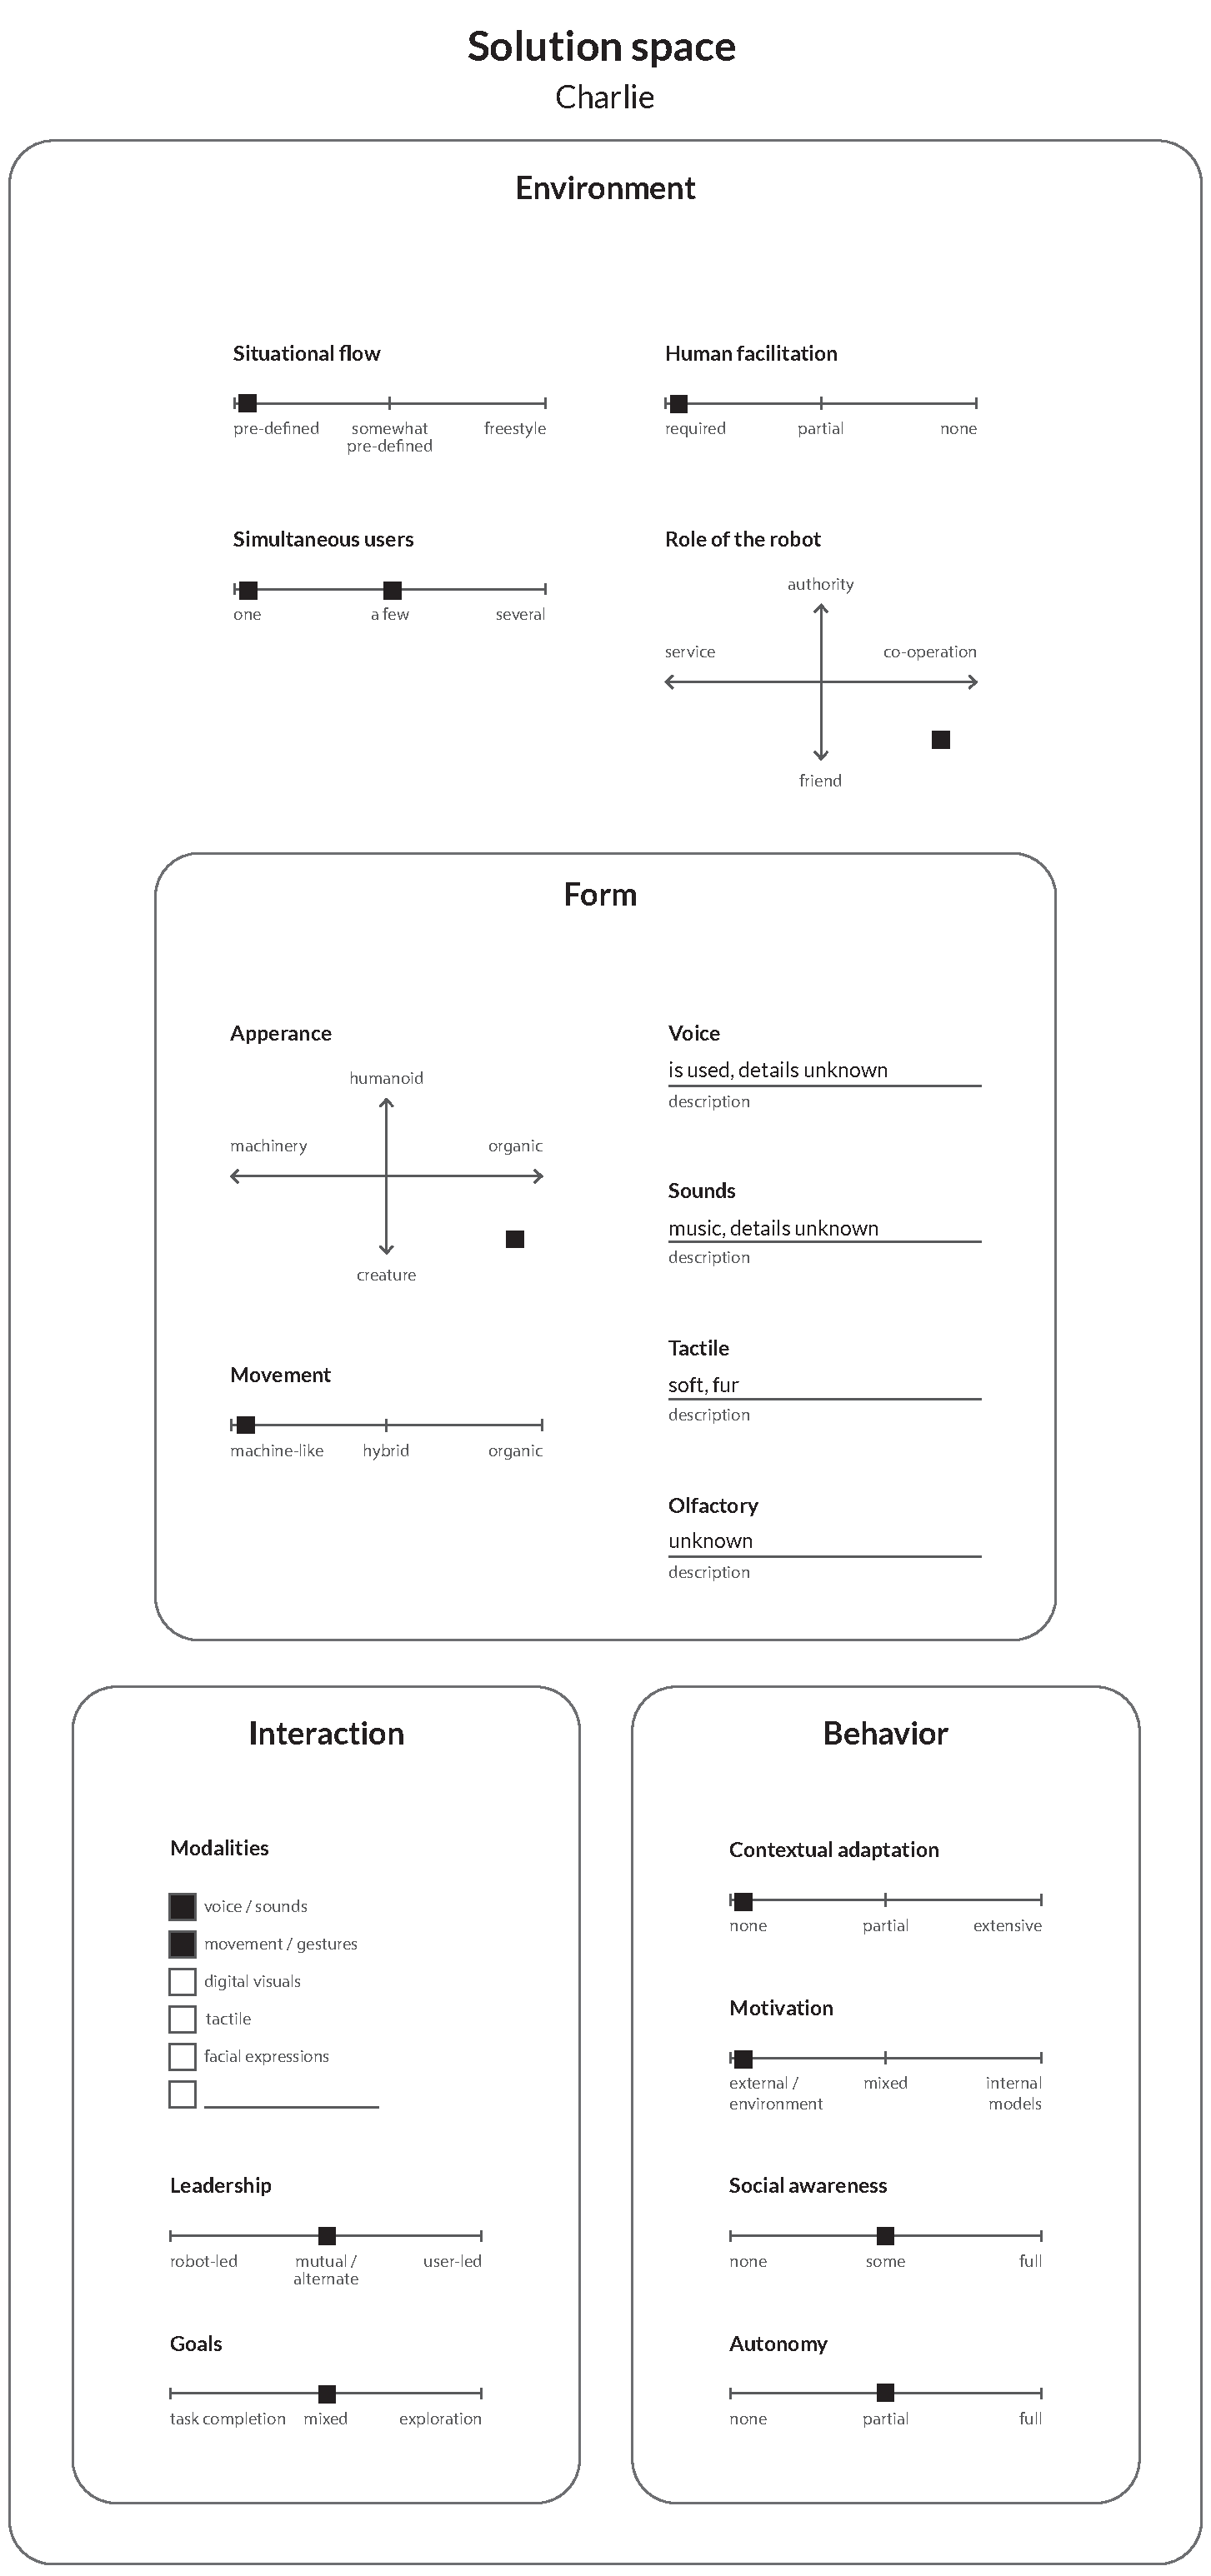
\includegraphics[scale=0.40]{images/solution_charlie-01.pdf}
  \caption{The robot Charlie is situated into the design framework.}
  \label{fig:charlieDesign}
\end{figure}

%%%%%%%%%%%%%

\chapter{Keepon in the design framework}
\label{chapter:keeponDesign}

The robot Keepon, introduced in chapter \ref{chapter:background}, was developed to study human-robot interaction with children, and was adapted to study interaction with children with autism. Keepon is situated into the design framework introduced in chapter \ref{chapter:design}, in order to showcase how the framework defines an existing robot, which was not designed specifically for use by children with autism. The implementation depicted in the framework (figure \ref{fig:keeponDesign} is based on the most recent study \cite{kozima2009keepon}.

The situational flow is described as freestyle, in contrast to both the InMoov described in this thesis and Charlie, which is detailed in chapter \ref{chapter:charlieDesign}. The Keepon was placed into a daycare for children with special needs, and autistic children could interact with it there sporadically. The study does not describe adults or other humans guiding the children to use the robot, but the Keepon was deliberately placed in the daycare among other toys. This means that there was partial human facilitation in the environment. The kids could explore the robot by themselves, or a few children could interact with it simultaneously. Children may also have interacted with the Keepon with their parent, or with a therapist.

The Keepon's form and manner of communication are very creature-like. It does not speak, and interacts by making chirping sounds, and moving to express its emotions. The Keepon's movements are quite organic, and do not appear robotic. 

The interactions were user-led, as the study did not detail Keepon initiating interactions \cite{kozima2009keepon}. The goal was for children to explore how the robot responds to them, meaning that goals were exploratory, and motivation for the robot's behavior was external. The study does not mention the robot exhibiting any improvisational behavior. The robot could operate both in an autonomous manner, or be fully controlled by a human, although the researchers mention that usually it was controlled by a human in studies with autistic children. No mention of the robot's socially aware qualities are made in the study \cite{kozima2009keepon}.





\begin{figure}
\centering
  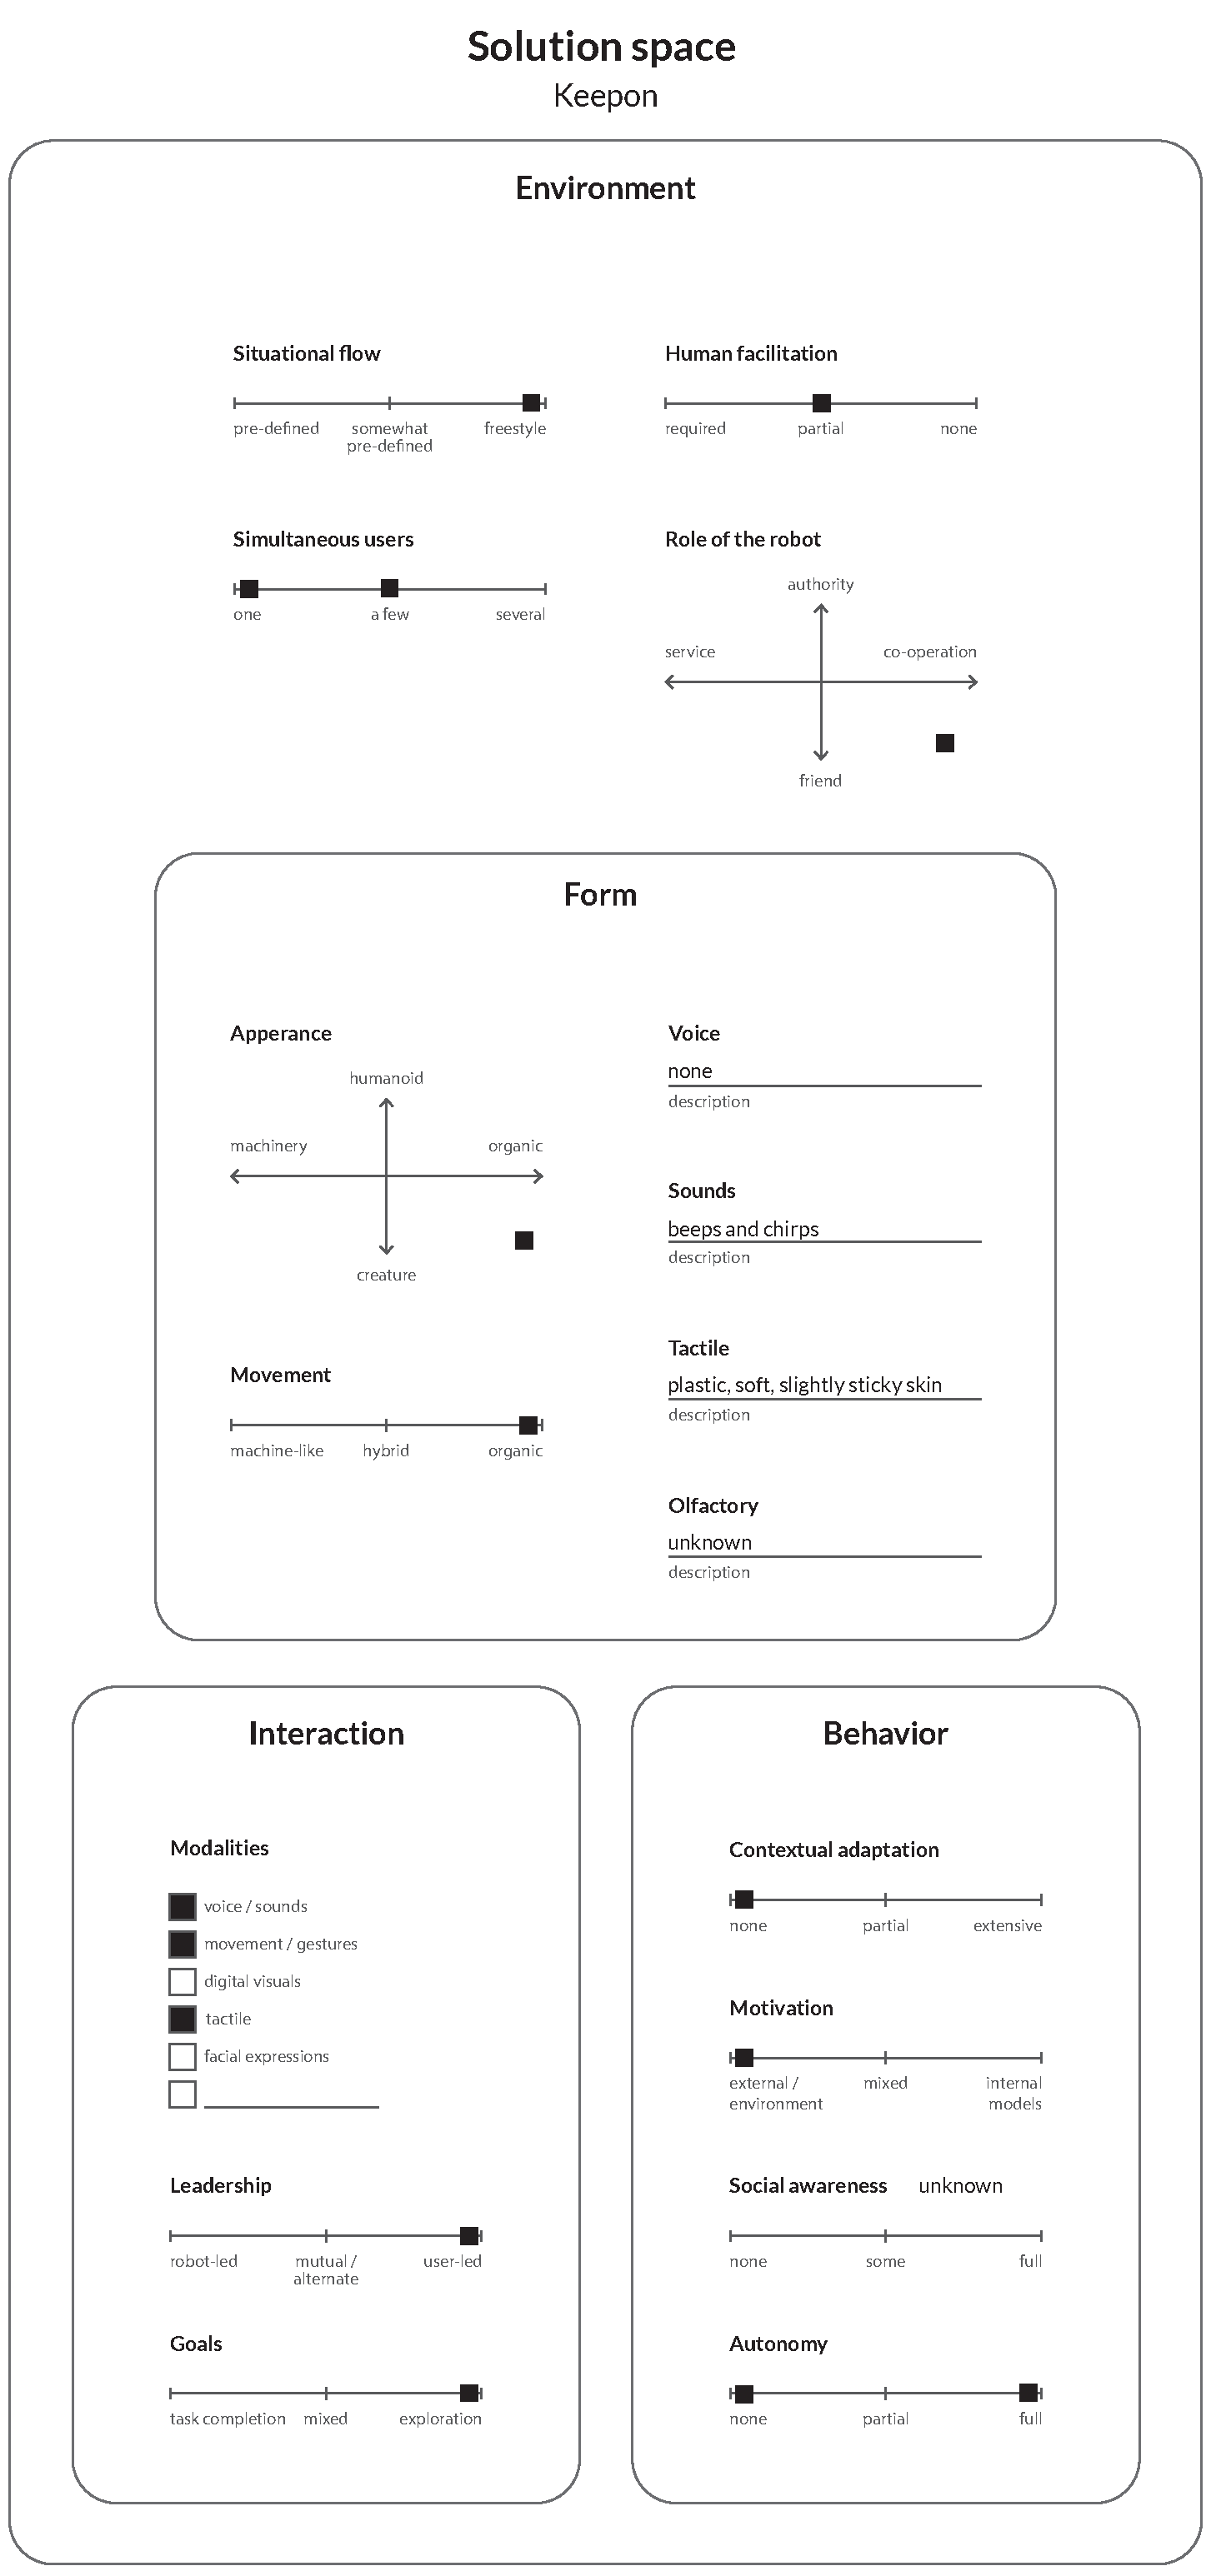
\includegraphics[scale=0.40]{images/solution_keepon-01.pdf}
  \caption{The robot Keepon is situated into the design framework.}
  \label{fig:keeponDesign}
\end{figure}

%%%%%%%%%%%%%%


\chapter{Explanation for children}
\label{chapter:explanation}

An explanation of the events to take place before, during and after the experiments was provided at the start of the experiment by the speech therapist. The symbols used are PECS-images, which are symbols frequently used by people with ASDs to communicate. The meaning of the images are written in Finnish below them.

\begin{figure}
\centering
  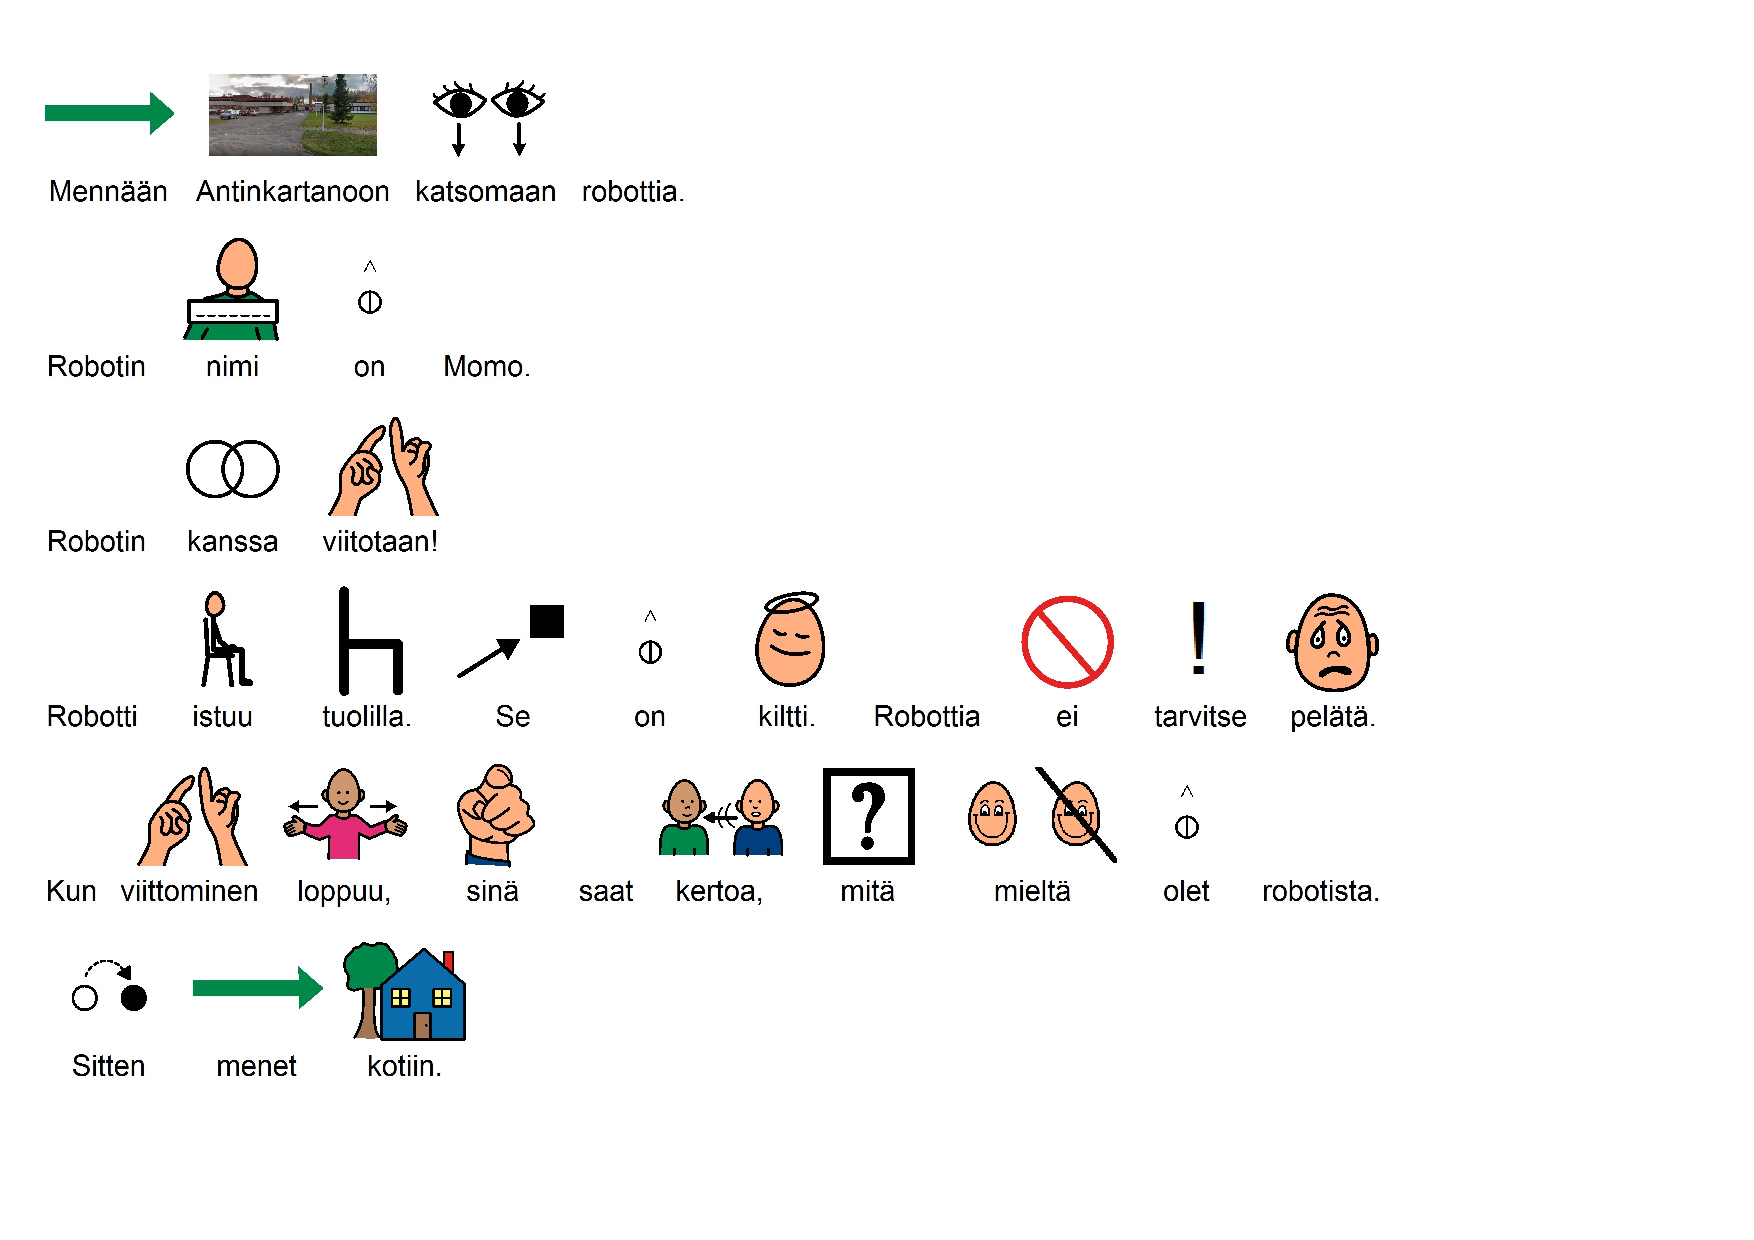
\includegraphics[scale=0.60, angle=-90]{images/kirje_lapselle.pdf}
  \caption{Explanation of the experiments for the children.}
  \label{fig:kirjelapselle}
\end{figure}



%%%



\chapter{Robot and child model conversation transcript}
\label{chapter:conversation}


\section{Esittely}
\begin{tabular}{llp{10cm}}
 1. & Robotti: & Hei, olen Momo. Olen robotti. \\
 2. &   & *robotti heiluttaa kättä tervehtimisen merkiksi* \\
 3. & Robotti: & Mikä sinun nimesi on? \\
 4. & Lapsi: & (nimi).\\
 5. & Robotti: & Hei, (nimi).\\
 6. & Robotti: & Tehdään yhdessä tehtäviä.\\
 7. & Robotti: & Katso, mitä minä teen. Tee sama perässä.\\
\end{tabular}

\section{Robotin viittoma}
\begin{tabular}{llp{10cm}}
 1. &  & *robotti viittoo* \\
 2. & & *jos tarve, robotti vilkuttaa valoa, tai näyttää tabletista kuvan* \\
 3. & Robotti: & (viittoman sana). \\
 4. & Robotti: & Nyt on sinun vuorosi. Tee samoin. \\
\end{tabular}


\section{Robotin reaktio}

Lapsi viittoo joko viittoo oikein, viittoo väärin, tai ei reagoi.

\subsection{Lapsi viittoo oikein}
\begin{tabular}{llp{10cm}}
 1. &  & *robotti näyttää peukkua ylös* \\
 2. & Robotti: & Hyvä, oikein meni.\\
 3. & Robotti: & Kokeillaan seuraavaa viittomaa.  \\
\end{tabular}

%%

\subsection{Lapsi viittoo väärin}
\begin{tabular}{llp{10cm}}
 1. & Robotti: & Hyvä yritys, ei mennyt ihan oikein. \\
 2. & Robotti: & Kokeillaan uudestaan. \\
 3. & & *robotti viittoo* \\
 4. & & *jos tarve, robotti vilkuttaa valoa, tai näyttää tabletista kuvan* \\
 5. & Robotti: & (viittoman sana). \\
 6. & Robotti: & Nyt on sinun vuorosi. Tee samoin. \\
 7. & & *odotetaan puheterapeutin indikoima aika* \\
\end{tabular}

\subsubsection{Lapsi viittoo nyt oikein}
\begin{tabular}{llp{10cm}}
 1. &  & *robotti näyttää peukkua ylös* \\
 2. & Robotti: & Hyvä, oikein meni.\\
 3. & Robotti: & Kokeillaan seuraavaa viittomaa.  \\
\end{tabular}

\subsubsection{Lapsi viittoo uudelleen väärin, tai ei reagoi}
\begin{tabular}{llp{10cm}}
 1. & Robotti: & Akuliina auttaa sinua nyt.\\
 2. & & *puheterapeutti näyttää viittoman, tai auttaa lasta tekemään sen kädestä pitäen* \\
 3. & Robotti: & Noin, nythän se onnistui.\\
 4. & Robotti: & Kokeillaan seuraavaa viittomaa.  \\
\end{tabular} \hfill\break

Joissakin tapauksissa lapsi ei saanut puheterapeutin avulla viittomaa oikein, jolloin repliikki 3 jätettiin sanomatta, ja siirrytiin suoraan repliikkiin 4.

%%

\subsection{Lapsi ei reagoi}
\begin{tabular}{llp{10cm}}
 1. & Robotti: & Hei, toista perässä mitä teen.. \\
 2. & & *robotti viittoo* \\
 3. & & *jos tarve, robotti vilkuttaa valoa, tai näyttää tabletista kuvan* \\
 4. & Robotti: & (viittoman sana). \\
 5. & Robotti: & Nyt on sinun vuorosi. Tee samoin. \\
 6. & & *odotetaan puheterapeutin indikoima aika* \\
\end{tabular}

\subsubsection{Lapsi viittoo nyt oikein}
\begin{tabular}{llp{10cm}}
 1. &  & *robotti näyttää peukkua ylös* \\
 2. & Robotti: & Hyvä, oikein meni.\\
 3. & Robotti: & Kokeillaan seuraavaa viittomaa.  \\
\end{tabular}

\subsubsection{Lapsi viittoo väärin, tai ei reagoi}
\begin{tabular}{llp{10cm}}
 1. & Robotti: & Akuliina auttaa sinua nyt.\\
 2. & & *puheterapeutti näyttää viittoman, tai auttaa lasta tekemään sen kädestä pitäen* \\
 3. & Robotti: & Noin, nythän se onnistui.\\
 4. & Robotti: & Kokeillaan seuraavaa viittomaa.  \\
\end{tabular} \hfill \break

Joissakin tapauksissa lapsi ei saanut puheterapeutin avulla viittomaa oikein, jolloin repliikki 3 jätettiin sanomatta, ja siirrytiin suoraan repliikkiin 4.

%%%

\section{Hyvästely}


\begin{tabular}{llp{10cm}}
 1. & Robotti: & Kiitos, minulla oli hauskaa.\\
 2. &  & *robotti heiluttaa kättää hyvästelemisen merkiksi*\\
 3. & Robotti: & Hei hei!  \\
\end{tabular}


%%%

\chapter{Survey for children}
\label{chapter:children}

After the experiments, the neurospychologist entered the experimentation room, and asked children to answer simple questions with the help of PECS-images.

\begin{figure}
\centering
  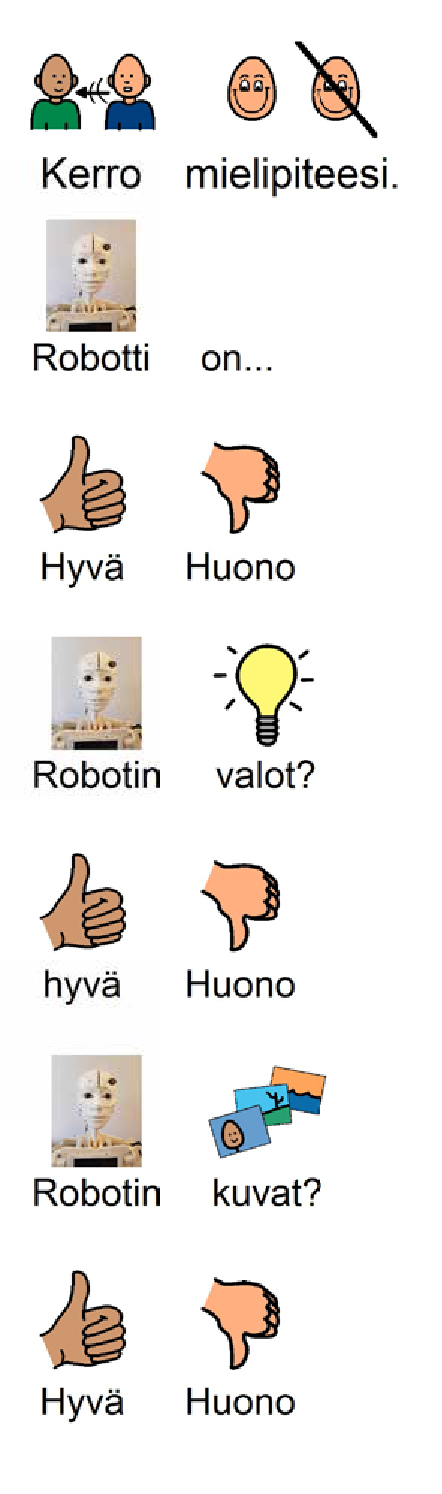
\includegraphics[scale=0.60]{images/kysely_lapselle_1.pdf}
  \caption{The first part of the survey for the children. The questions are: "Give your opinion." "The robot is... Good or bad?", "The robot's lights are... Good or bad?", "The robot's images are... Good or bad?"}
  \label{fig:kirjelapselle1}
\end{figure}

\begin{figure}
\centering
  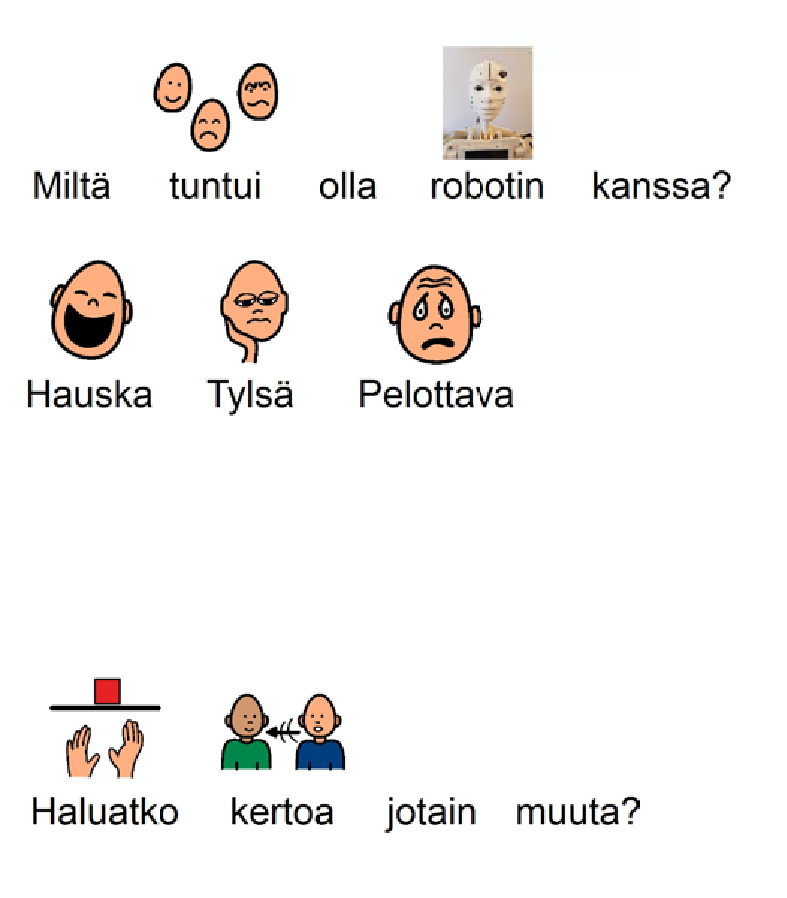
\includegraphics[scale=0.60]{images/kysely_lapselle_2.pdf}
  \caption{The second part of the survey for the children. The questions are: "How did it feel to be with the robot? Fun, boring, or scary?", "Do you want to tell something else?"}
  \label{fig:kirjelapselle2}
\end{figure}


%%%


\chapter{Survey for companions}
\label{chapter:companions}

After the experiments, the childrens' companions were given a survey to fill out. Some of the companions filled it immediately, and some returned it later by post. Companions were either childrens' parents, or therapists familiar with them. The surveys are in Finnish.

The questions are:
\begin{itemize}
  \item How did your child experience the situation? Fun, scary, boring, something else?
  \item How did you feel during the experiment? Fun, scary, boring, something else?
  \item Did you think your child had a connection with the robot? Yes or no.
  \item How did you perceive your child to have a connection with the robot when compared to a human? Better than with a human, same as with a human, worse than with a human.
  \item Do you think your child could benefit from practicing with the robot?
  \item Why or why not?
  \item What was the best and worst design condition (1. for best, 3. for worst)? Sign + sound, sign + sound + lights, sign + sound + image.
  \item What did you think of the design conditions? What was good and what was bad? Why? Sign + sound, sign + sound + lights, sign + sound + image.
  \item Do you have other things to say about the design conditions?
  \item Free word.
\end{itemize}

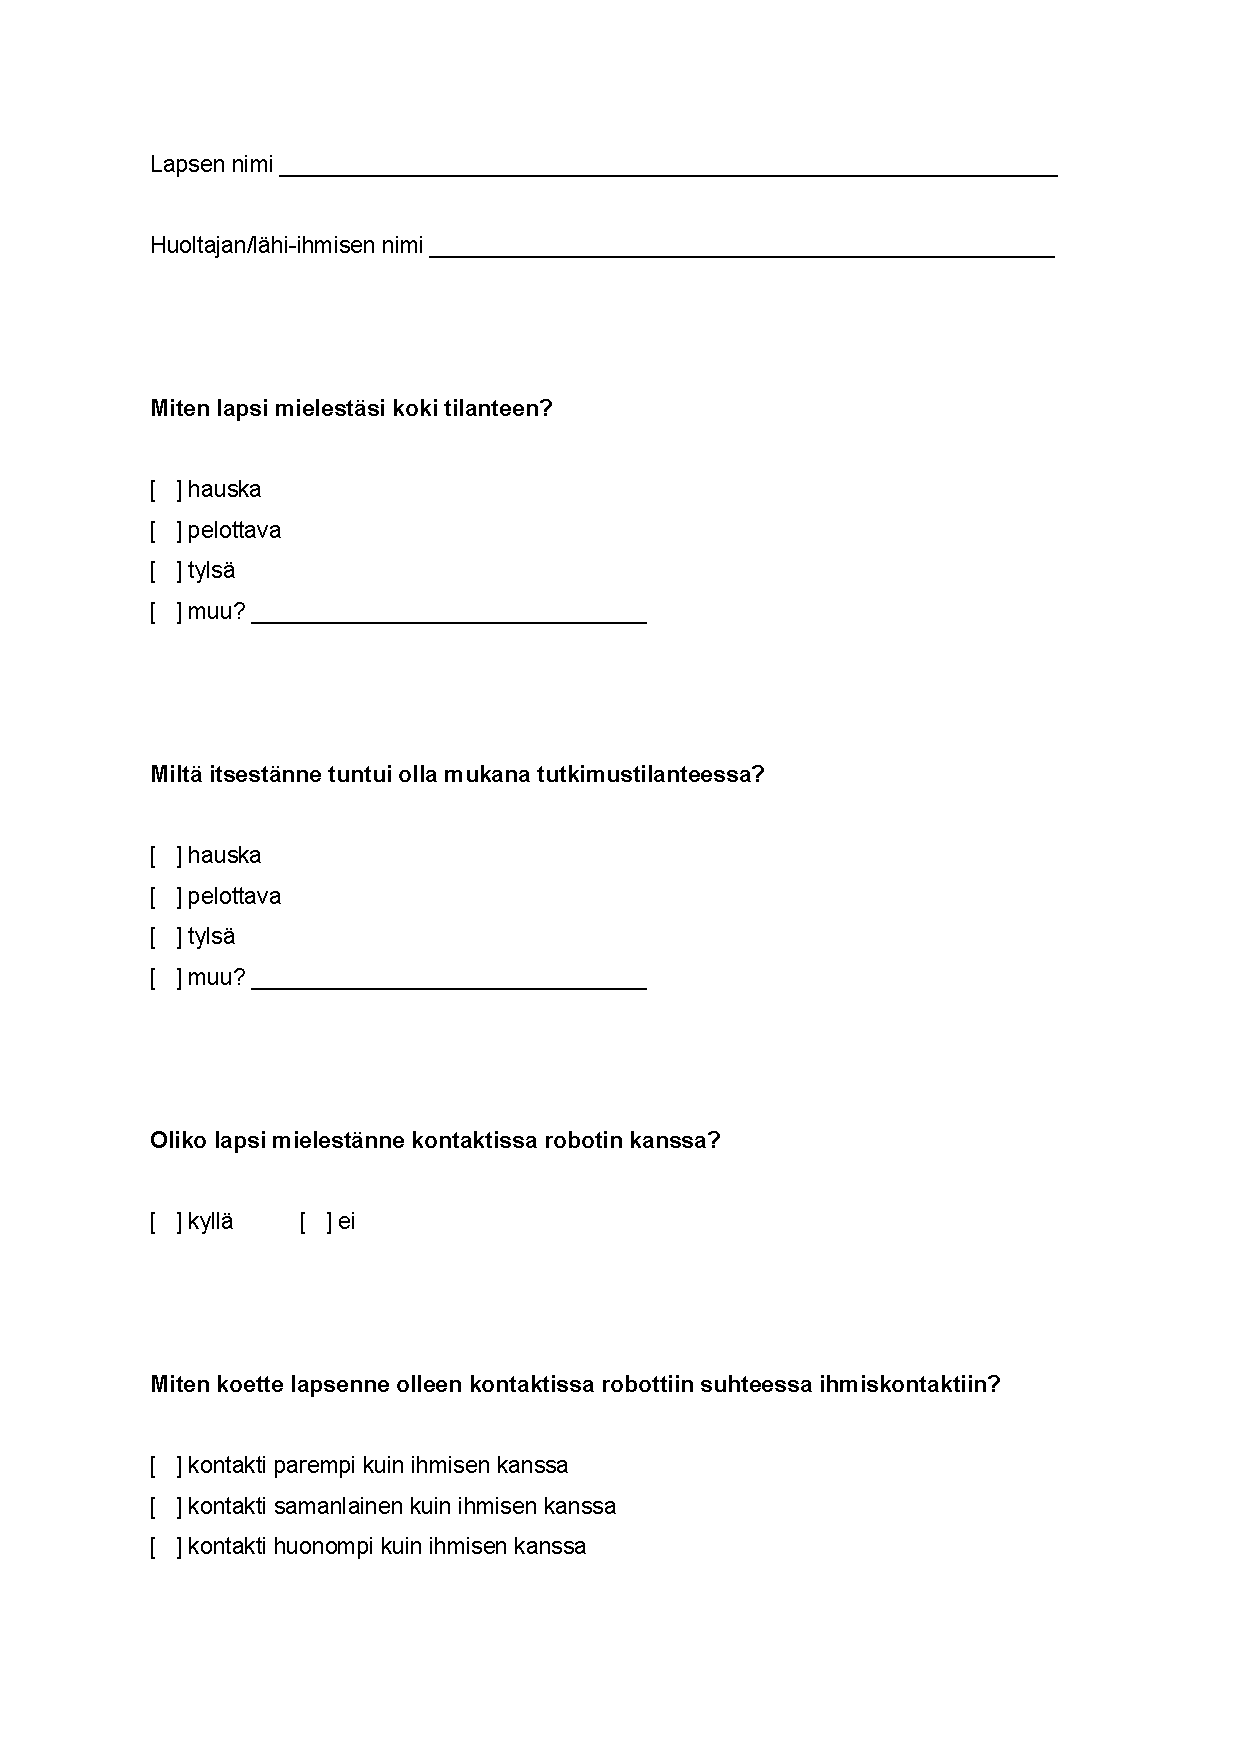
\includepdf[pages=-]{images/kysely_vanhemmille.pdf}


%%%

%For now, the Aalto logo variants are shown in Figure~\ref{fig:aaltologo}.

%\begin{figure}
%\begin{center}
%\subfigure[In English]{
\includegraphics[width=.8\textwidth]{images/aalto-logo-en}}
%\subfigure[Suomeksi]{
\includegraphics[width=.8\textwidth]{images/aalto-logo-fi}}
%\subfigure[På svenska]{
\includegraphics[width=.8\textwidth]{images/aalto-logo-se}}
%\caption{Aalto logo variants}
%\label{fig:aaltologo}
%\end{center}
%\end{figure}


% End of document!
% ------------------------------------------------------------------
% The LastPage package automatically places a label on the last page.
% That works better than placing a label here manually, because the
% label might not go to the actual last page, if LaTeX needs to place
% floats (that is, figures, tables, and such) to the end of the 
% document.


\end{document}
